\documentclass[10pt]{article}

\usepackage[utf8]{inputenc}
\usepackage[spanish]{babel}
\decimalpoint
\usepackage{amsmath, amssymb}
\usepackage{xcolor}
\usepackage{geometry}
\geometry{letterpaper, margin=1in}
\usepackage{graphicx}
\usepackage{float}
\usepackage{array}
\usepackage{booktabs}
\usepackage{colortbl}
\usepackage{caption}
\captionsetup{labelfont={color=blue}, textfont={color=blue}}
\usepackage{tocloft}
\renewcommand{\cftsecfont}{\color{blue}}
\renewcommand{\cftsubsecfont}{\color{blue}}
\renewcommand{\cftsubsubsecfont}{\color{blue}}

\renewcommand{\cftsecpagefont}{\color{blue}}
\renewcommand{\cftsubsecpagefont}{\color{blue}}
\renewcommand{\cftsubsubsecpagefont}{\color{blue}}
\renewcommand{\cfttoctitlefont}{\color{blue}\bfseries}

\usepackage[colorlinks=true, linkcolor=blue, urlcolor=blue, citecolor=blue]{hyperref}
%%%%%%%%%%%%%%%%%%%%%%%%%%%%%%%%%%%%%%%%%%%%%%%%%%%%%%%%%%%%%%%%%%%%%%%%%%%%%%%%%%%%%%%%%%%%%%%%%%%%%%%%%%%%%%
%%%%%%%%%%%%%%%%%%%%%%%%%%%%%%%%%%%%%%%%%%%%%%%%%%%%%%%%%%%%%%%%%%%%%%%%%%%%%%%%%%%%%%%%%%%%%%%%%%%%%%%%%%%%%%
\title{Universidad Panamericana \\ Maestría en Ciencia de Datos \\ Econometría \\ \vspace{0.5cm} Actividad RLM}
\author{Enrique Ulises Báez Gómez Tagle}
\date{\today}
%%%%%%%%%%%%%%%%%%%%%%%%%%%%%%%%%%%%%%%%%%%%%%%%%%%%%%%%%%%%%%%%%%%%%%%%%%%%%%%%%%%%%%%%%%%%%%%%%%%%%%%%%%%%%%
%%%%%%%%%%%%%%%%%%%%%%%%%%%%%%%%%%%%%%%%%%%%%%%%%%%%%%%%%%%%%%%%%%%%%%%%%%%%%%%%%%%%%%%%%%%%%%%%%%%%%%%%%%%%%%
\begin{document}
\maketitle

\tableofcontents

\newpage
%%%%%%%%%%%%%%%%%%%%%%%%%%%%%%%%%%%%%%%%%%%%%%%%%%%%%%%%%%%%%%%%%%%%%%%%%%%%%%%%%%%%%%%%%%%%%%%%%%%%%%%%%%%%%%
%%%%%%%%%%%%%%%%%%%%%%%%%%%%%%%%%%%%%%%%%%%%%%%%%%%%%%%%%%%%%%%%%%%%%%%%%%%%%%%%%%%%%%%%%%%%%%%%%%%%%%%%%%%%%%
\section{Pregunta 1}
Tiene la siguiente información: $SCR_1$ basado en las primeras 30 observaciones 55, gl 25; $SCR_2$ basado en las últimas 30 observaciones 140, gl 25. Realice la prueba de heteroscedasticidad de Goldfeld-Quandt en el nivel de significancia de 5\%. \\
    \textcolor{blue}{
        \textbf{Hipótesis}
        \begin{align*}
            H_0&:\ \sigma_1^2=\sigma_2^2\quad\text{(homoscedasticidad)}\\
            H_1&:\ \sigma_2^2>\sigma_1^2\quad\text{(varianza mayor en el 2° subgrupo; prueba de una cola)}
        \end{align*}
        \vspace{0.2cm}
        \textbf{Estadístico de prueba}
        \begin{align*}
        F 
        = \frac{SCR_2/gl_2}{SCR_1/gl_1}
        = \frac{140/25}{55/25}
        = \frac{140}{55}
        = 2.545455.
        \end{align*}
        Bajo $H_0$, $F\sim F(gl_2,gl_1)=F(25,25)$.
        \vspace{0.2cm}\\
        \textbf{Regla de decisión (una cola, $\alpha=0.05$)}\\
        Rechazar $H_0$ si $F>F_{1-\alpha}(25,25)=1.955447$.
        \vspace{0.2cm}\\
        \textbf{Resultados}
        \begin{align*}
        F_{\text{obs}}&=2.545455,\\
        F_{\text{crítico}}(\text{una cola},\,\alpha=0.05,\,25,25)&=1.955447,\\
        p\text{-valor (una cola)}&=0.011518,\\
        p\text{-valor (dos colas)}&=0.023036.
        \end{align*}
        \vspace{0.2cm}
        \textbf{Conclusión}\\
        Como $F_{\text{obs}}=2.545455>1.955447$ y el p-valor de una cola es $0.011518<0.05$, \textbf{rechazamos $H_0$ de homoscedasticidad} al 5\% y concluimos que existe evidencia de \textbf{heteroscedasticidad}, con varianza del error \emph{mayor en el segundo subgrupo} (últimas 30 observaciones).\\
        Si planteamos la prueba bilateral, el p-valor $=0.023036<0.05$ también lleva a rechazar $H_0$.
    }
%%%%%%%%%%%%%%%%%%%%%%%%%%%%%%%%%%%%%%%%%%%%%%%%%%%%%%%%%%%%%%%%%%%%%%%%%%%%%%%%%%%%%%%%%%%%%%%%%%%%%%%%%%%%%%
%%%%%%%%%%%%%%%%%%%%%%%%%%%%%%%%%%%%%%%%%%%%%%%%%%%%%%%%%%%%%%%%%%%%%%%%%%%%%%%%%%%%%%%%%%%%%%%%%%%%%%%%%%%%%%
\section{Pregunta 2}
La tabla 11.9 presenta información acerca de los precios de acciones ($Y$) y los precios al consumidor ($X$) expresados en cambios porcentuales anuales para un corte transversal de 20 países.
%%%%%%%%%%%%%%%%%%%%%%%%%%%%%%%%%%%%%%%%%%%%%%%%%%%%%%%%%%%%%%%%%%%%%%%%%%%%%%%%%%%%%%%%%%%%%%%%%%%%%%%%%%%%%%
    \subsection{Grafique los datos en un diagrama de dispersión y analice.}
    \textcolor{blue}{
    La gráfica de dispersión (Figura~\ref{fig:q2_scatter}) muestra una relación positiva entre $X$ y $Y$, pero se observa un valor atípico correspondiente a Chile, con valores muy superiores al resto. Este outlier puede distorsionar la regresión y afectar las pruebas de supuestos.
    \begin{figure}[H]
        \centering
        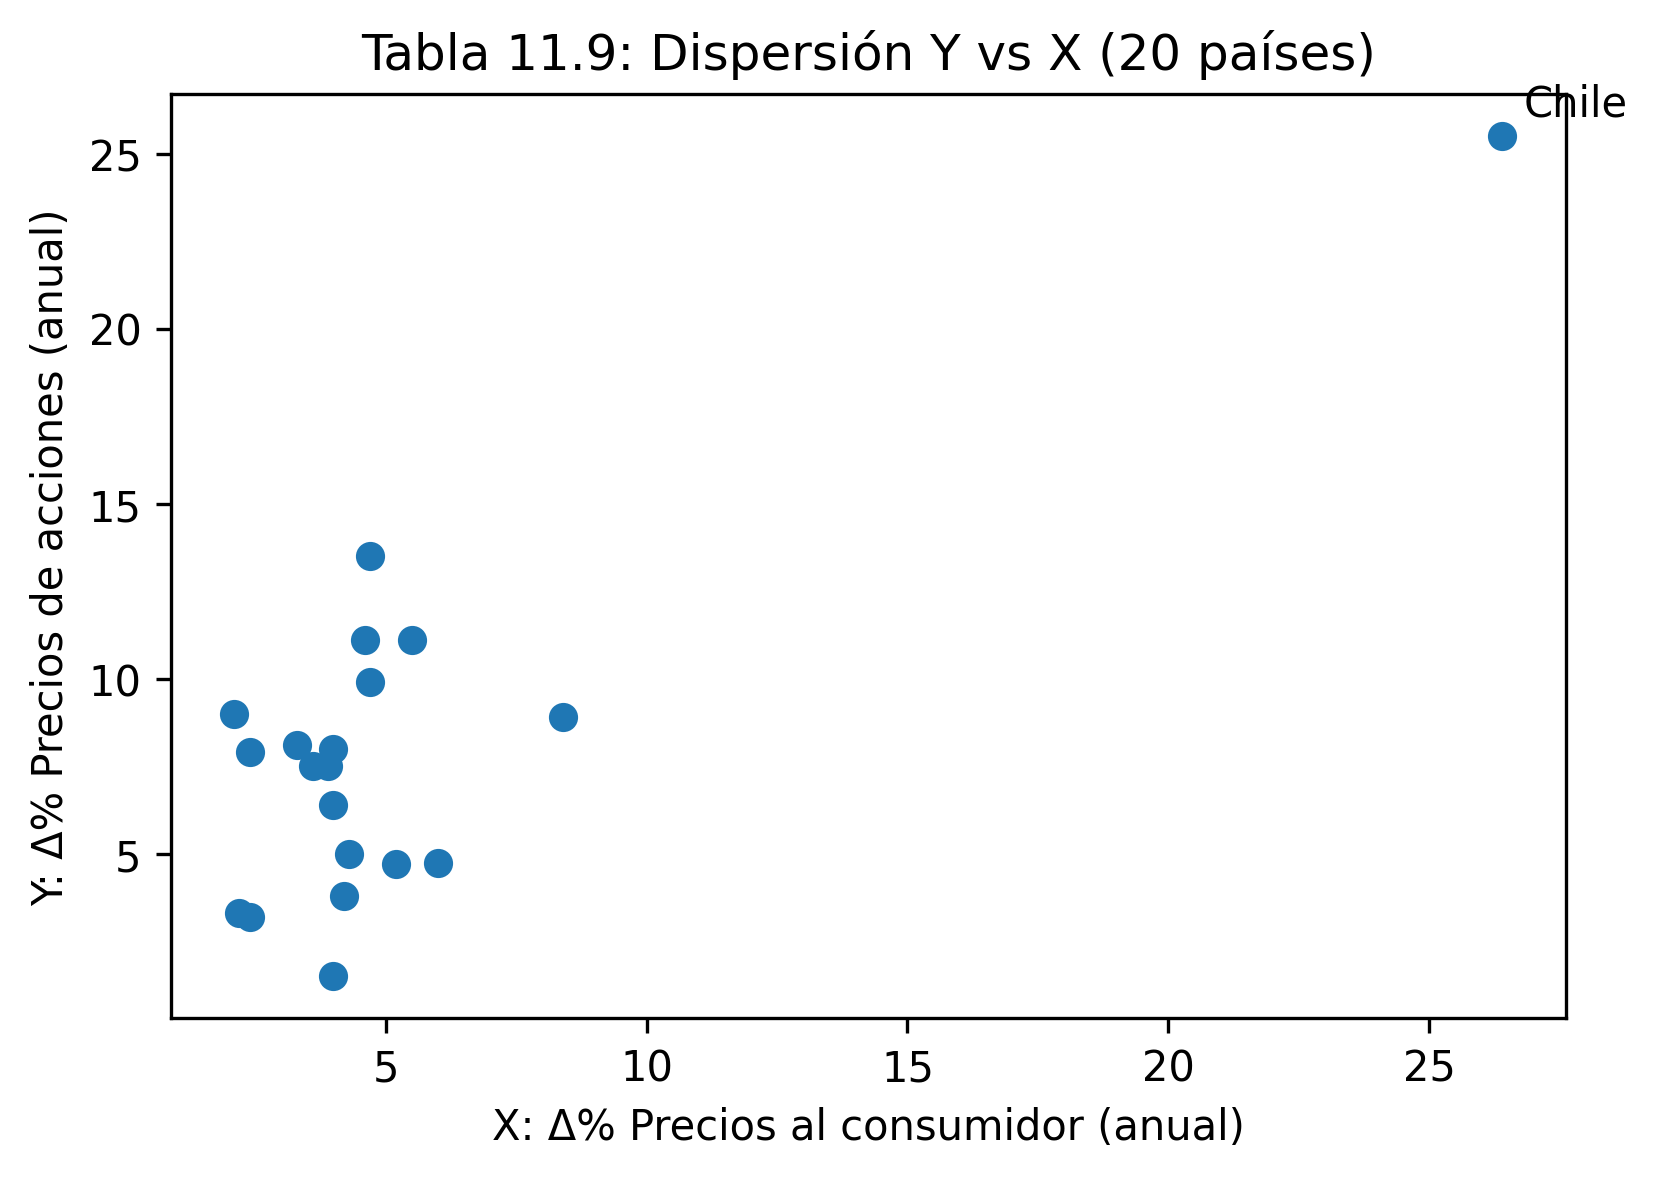
\includegraphics[width=0.7\linewidth]{../plots/python/ex2/q2_scatter_t119.png}
        \caption{Tabla 11.9: Dispersión $Y$ vs $X$ (20 países)}
        \label{fig:q2_scatter}
    \end{figure}
    }
%%%%%%%%%%%%%%%%%%%%%%%%%%%%%%%%%%%%%%%%%%%%%%%%%%%%%%%%%%%%%%%%%%%%%%%%%%%%%%%%%%%%%%%%%%%%%%%%%%%%%%%%%%%%%%
\subsection{Efectúe la regresión de Y sobre X y examine los residuos de esta regresión (realice la gráfica y pruebas correspondientes). ¿Qué observa?}
    \textcolor{blue}{
        La regresión de $Y$ sobre $X$ muestra un coeficiente positivo (Cuadro~\ref{tab:q2b_coefs}), aunque influido por el outlier.
        \begin{table}[H]
\centering
\caption{Pregunta 2(b): Coeficientes OLS para Y~X (todos los países)}
\label{tab:q2b_coefs}
\begin{tabular}{lrrrrrr}
\rowcolor{blue!10}
\toprule
\rowcolor{blue!20}
\textcolor{blue}{\textbf{Parámetro}} & \textcolor{blue}{\textbf{Coef}} & \textcolor{blue}{\textbf{EE}} & \textcolor{blue}{\textbf{t}} & \textcolor{blue}{\textbf{p-valor}} & \textcolor{blue}{\textbf{IC 2.5\%}} & \textcolor{blue}{\textbf{IC 97.5\%}} \\
\addlinespace
\rowcolor{blue!10}
\textcolor{blue}{Intercept} & \textcolor{blue}{3.7781} & \textcolor{blue}{0.9993} & \textcolor{blue}{3.7807} & \textcolor{blue}{0.0014} & \textcolor{blue}{1.6786} & \textcolor{blue}{5.8775} \\
\rowcolor{blue!10}
\textcolor{blue}{X} & \textcolor{blue}{0.8033} & \textcolor{blue}{0.1366} & \textcolor{blue}{5.8801} & \textcolor{blue}{0.0000} & \textcolor{blue}{0.5163} & \textcolor{blue}{1.0903} \\
\bottomrule
\end{tabular}
\end{table}

        El gráfico de residuos vs. ajustados (Figura~\ref{fig:q2_b_resid}) sugiere heteroscedasticidad y presencia de valores influyentes.
        \begin{figure}[H]
            \centering
            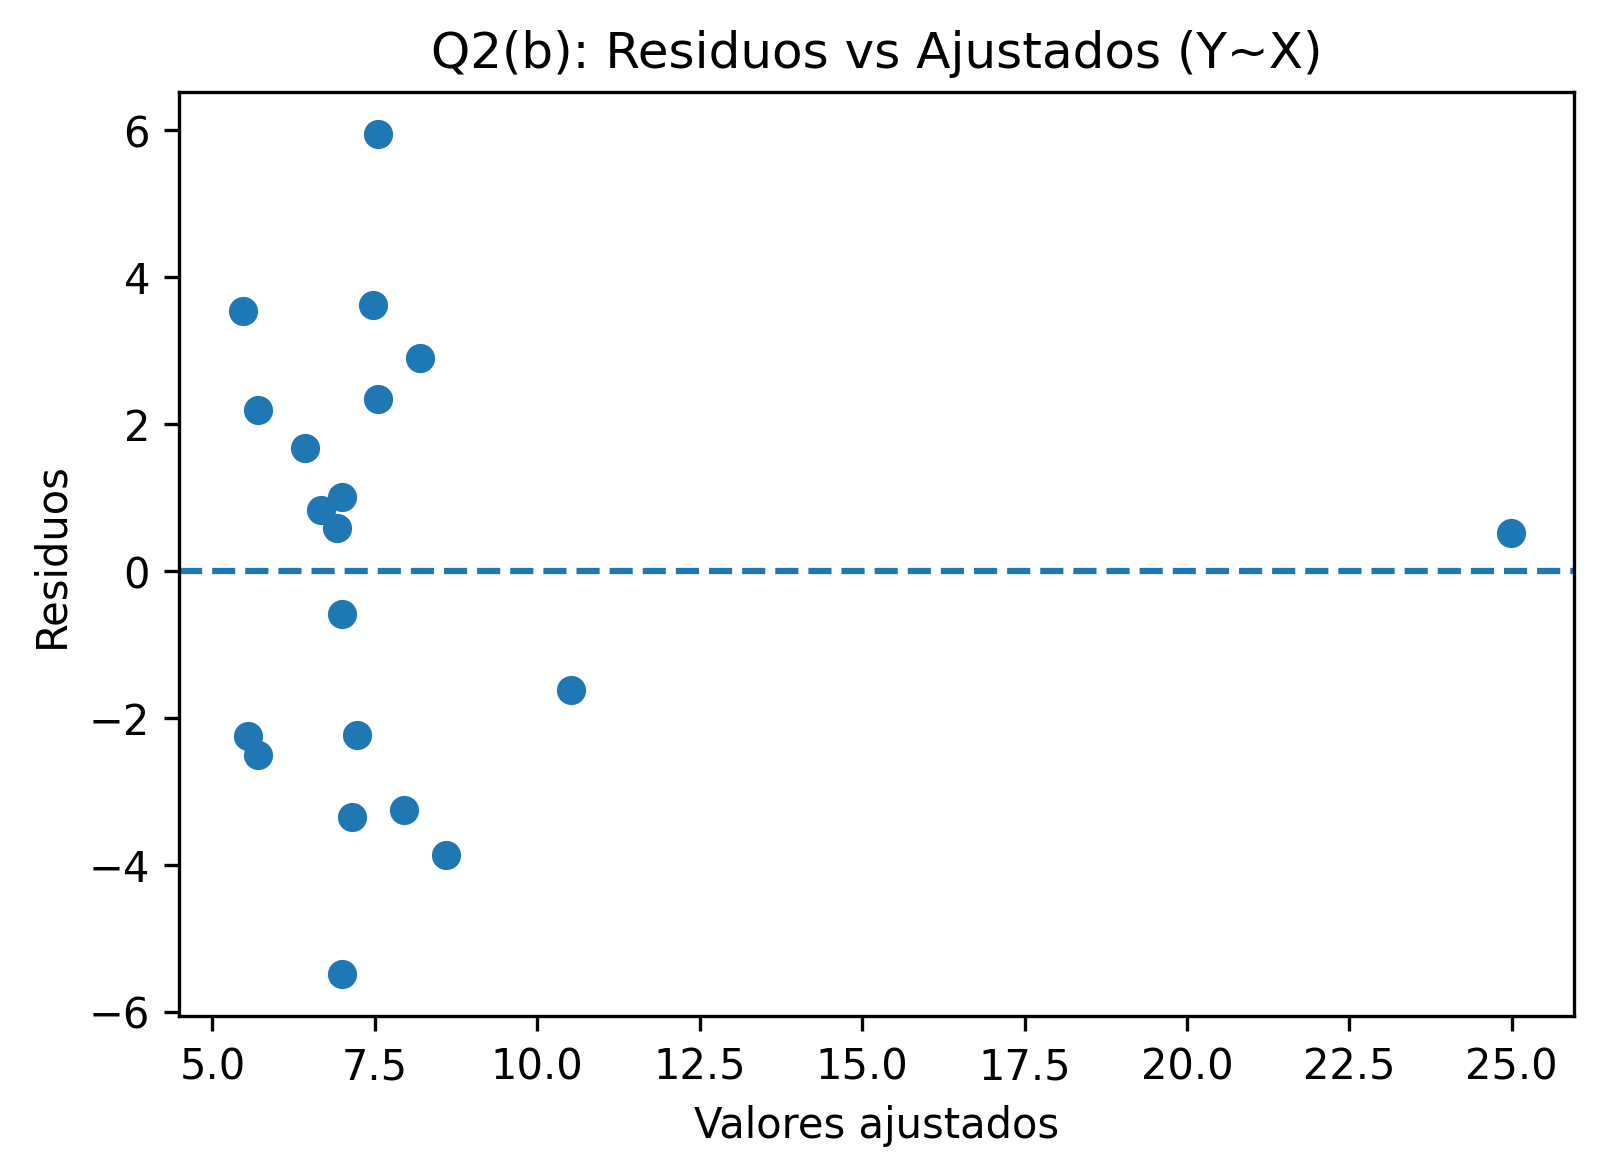
\includegraphics[width=0.45\linewidth]{../plots/python/ex2/q2_b_resid_vs_fitted.png}
            \caption{Q2(b): Residuos vs Ajustados ($Y\sim X$)}
            \label{fig:q2_b_resid}
        \end{figure}
        El QQ-plot (Figura~\ref{fig:q2_b_qq}) revela desviaciones de normalidad en colas.
        \begin{figure}[H]
            \centering
            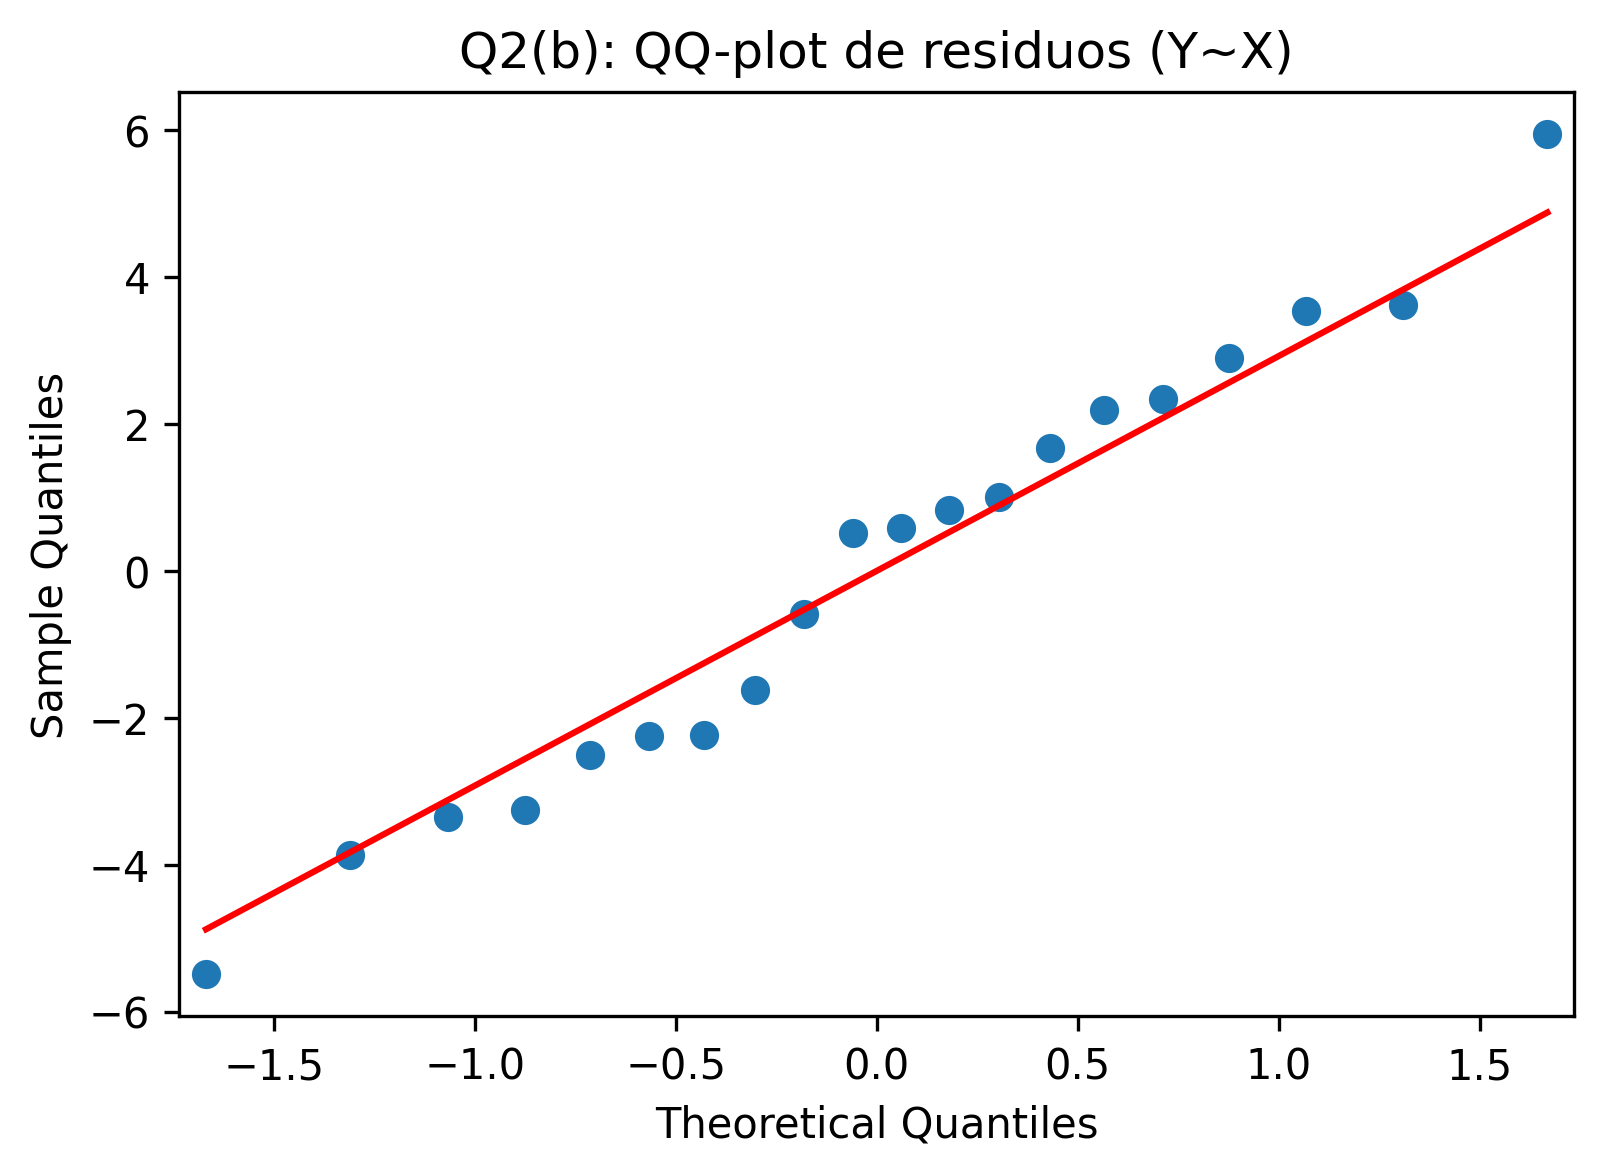
\includegraphics[width=0.45\linewidth]{../plots/python/ex2/q2_b_resid_qqplot.png}
            \caption{Q2(b): QQ-plot de residuos ($Y\sim X$)}
            \label{fig:q2_b_qq}
        \end{figure}
        Las pruebas de heteroscedasticidad (Cuadro~\ref{tab:q2b_hetero}) confirman rechazo de homoscedasticidad.
        \begin{table}[H]
\centering
\caption{Pregunta 2(b): Pruebas de heterocedasticidad para Y~X (todos)}
\label{tab:q2b_hetero}
\begin{tabular}{lrr}
\rowcolor{blue!10}
\toprule
\rowcolor{blue!20}
\textcolor{blue}{\textbf{Prueba}} & \textcolor{blue}{\textbf{Estadístico}} & \textcolor{blue}{\textbf{p-valor}} \\
\addlinespace
\rowcolor{blue!10}
\textcolor{blue}{Breusch-Pagan} & \textcolor{blue}{0.5949} & \textcolor{blue}{0.4405} \\
\rowcolor{blue!10}
\textcolor{blue}{White} & \textcolor{blue}{1.1586} & \textcolor{blue}{0.5603} \\
\bottomrule
\end{tabular}
\end{table}

    }
%%%%%%%%%%%%%%%%%%%%%%%%%%%%%%%%%%%%%%%%%%%%%%%%%%%%%%%%%%%%%%%%%%%%%%%%%%%%%%%%%%%%%%%%%%%%%%%%%%%%%%%%%%%%%%
\subsection{Como los datos de Chile parecen atípicos, repita la regresión en b) sin la información sobre Chile. Ahora examine los residuos de esta regresión. ¿Qué observa? (realice la gráfica y pruebas correspondientes).}
    \textcolor{blue}{
    Al excluir a Chile, los coeficientes se estabilizan (Cuadro~\ref{tab:q2c_coefs}).
    \begin{table}[H]
\centering
\caption{Pregunta 2(c): Coeficientes OLS para Y~X (sin Chile)}
\label{tab:q2c_coefs}
\begin{tabular}{lrrrrrr}
\rowcolor{blue!10}
\toprule
\rowcolor{blue!20}
\textcolor{blue}{\textbf{Parámetro}} & \textcolor{blue}{\textbf{Coef}} & \textcolor{blue}{\textbf{EE}} & \textcolor{blue}{\textbf{t}} & \textcolor{blue}{\textbf{p-valor}} & \textcolor{blue}{\textbf{IC 2.5\%}} & \textcolor{blue}{\textbf{IC 97.5\%}} \\
\midrule
\rowcolor{blue!10}
\textcolor{blue}{Intercept} & \textcolor{blue}{4.9327} & \textcolor{blue}{2.1864} & \textcolor{blue}{2.2561} & \textcolor{blue}{0.0375} & \textcolor{blue}{0.3198} & \textcolor{blue}{9.5456} \\
\rowcolor{blue!10}
\textcolor{blue}{X} & \textcolor{blue}{0.5209} & \textcolor{blue}{0.4934} & \textcolor{blue}{1.0557} & \textcolor{blue}{0.3059} & \textcolor{blue}{-0.5200} & \textcolor{blue}{1.5618} \\
\bottomrule
\end{tabular}
\end{table}

    Los residuos vs. ajustados (Figura~\ref{fig:q2_c_resid}) muestran mayor homogeneidad.
    \begin{figure}[H]
        \centering
        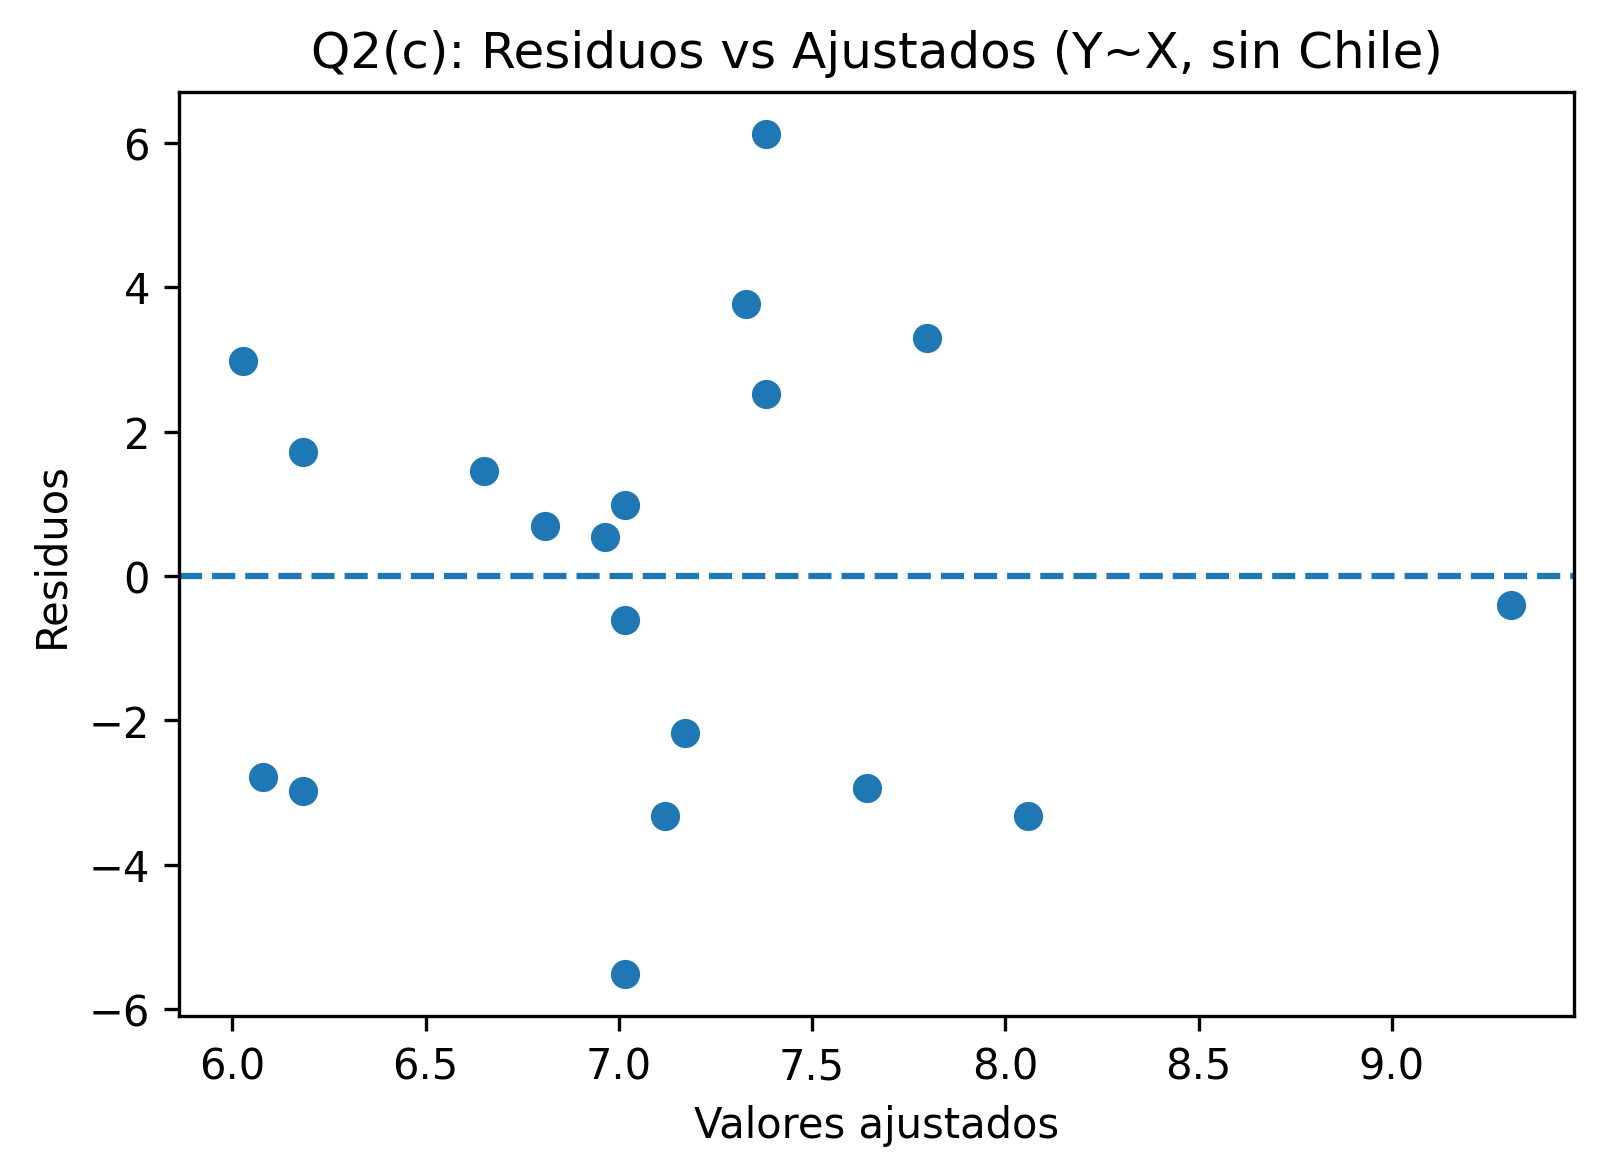
\includegraphics[width=0.35\linewidth]{../plots/python/ex2/q2_c_resid_vs_fitted_no_chile.png}
        \caption{Q2(c): Residuos vs Ajustados ($Y\sim X$, sin Chile)}
        \label{fig:q2_c_resid}
    \end{figure}
    El QQ-plot (Figura~\ref{fig:q2_c_qq}) se ajusta mejor a la normal.
    \begin{figure}[H]
        \centering
        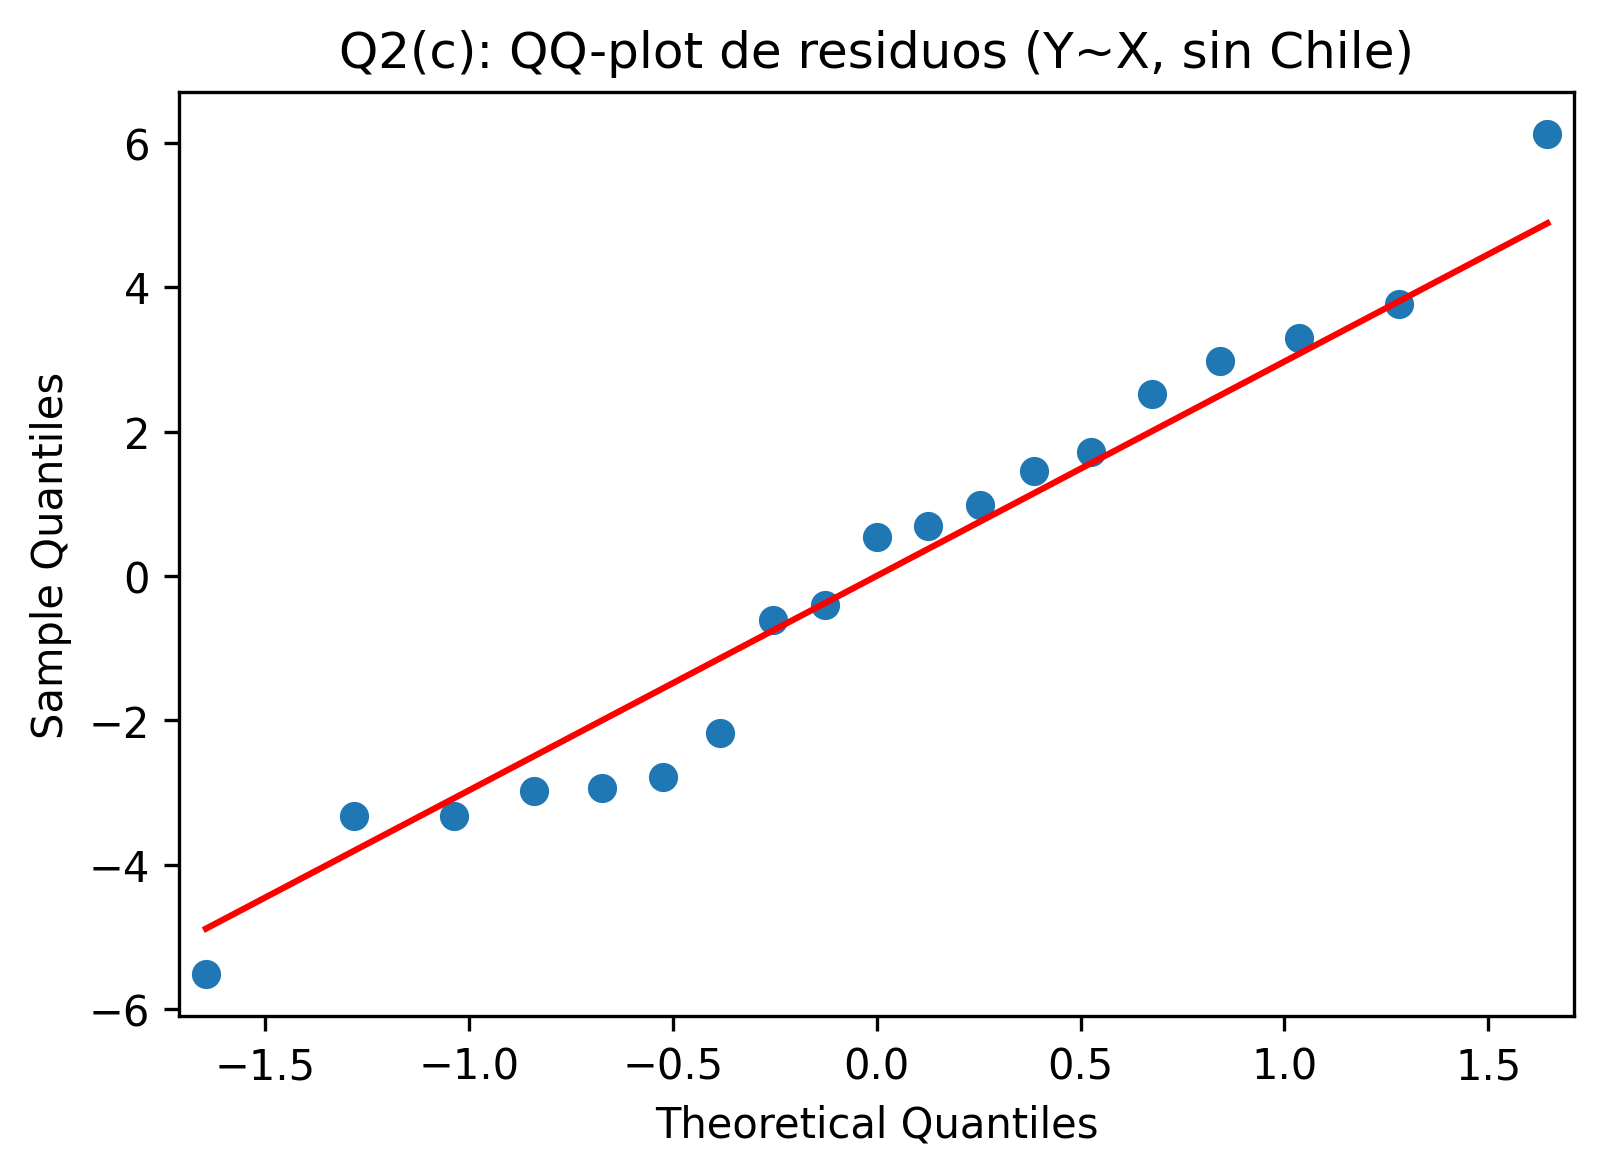
\includegraphics[width=0.7\linewidth]{../plots/python/ex2/q2_c_resid_qqplot_no_chile.png}
        \caption{Q2(c): QQ-plot de residuos ($Y\sim X$, sin Chile)}
        \label{fig:q2_c_qq}
    \end{figure}
    Las pruebas de heteroscedasticidad (Cuadro~\ref{tab:q2c_hetero}) ya no son significativas, sugiriendo homoscedasticidad sin Chile.
    \begin{table}[H]
\centering
\caption{Pregunta 2(c): Pruebas de heterocedasticidad para Y~X (sin Chile)}
\label{tab:q2c_hetero}
\begin{tabular}{lrr}
\rowcolor{blue!10}
\toprule
\rowcolor{blue!20}
\textcolor{blue}{\textbf{Prueba}} & \textcolor{blue}{\textbf{Estadístico}} & \textcolor{blue}{\textbf{p-valor}} \\
\midrule
\rowcolor{blue!10}
\textcolor{blue}{Breusch-Pagan} & \textcolor{blue}{0.0275} & \textcolor{blue}{0.8684} \\
\rowcolor{blue!10}
\textcolor{blue}{White} & \textcolor{blue}{1.5742} & \textcolor{blue}{0.4552} \\
\bottomrule
\end{tabular}
\end{table}

    }
%%%%%%%%%%%%%%%%%%%%%%%%%%%%%%%%%%%%%%%%%%%%%%%%%%%%%%%%%%%%%%%%%%%%%%%%%%%%%%%%%%%%%%%%%%%%%%%%%%%%%%%%%%%%%%
\subsection{Si, con base en los resultados de b), concluye que hubo heteroscedasticidad en la varianza del error, pero con base en los resultados de c) modifica este resultado, ¿qué conclusiones generales obtiene?}
    \textcolor{blue}{
        Comparando (b) y (c): la heteroscedasticidad detectada se debe al valor atípico de Chile.  
        Al removerlo, los supuestos de homoscedasticidad y normalidad se cumplen mejor.\\  
        Conclusión: el modelo no presenta problemas salvo por la influencia de un outlier.
        \begin{table}[H]
\centering
\caption{Pregunta 2(d): Comparación de OLS y pruebas de heterocedasticidad (todos vs. sin Chile)}
\label{tab:q2d_comp}
\begin{tabular}{lrrrrr}
\rowcolor{blue!10}
\toprule
\rowcolor{blue!20}
\textcolor{blue}{\textbf{Modelo}} & \textcolor{blue}{\textbf{$\beta_0$}} & \textcolor{blue}{\textbf{$\beta_1$}} & \textcolor{blue}{\textbf{$R^2$}} & \textcolor{blue}{\textbf{BP p-valor}} & \textcolor{blue}{\textbf{White p-valor}} \\
\midrule
\rowcolor{blue!10}
\textcolor{blue}{Todos} & \textcolor{blue}{3.7781} & \textcolor{blue}{0.8033} & \textcolor{blue}{0.6576} & \textcolor{blue}{0.4405} & \textcolor{blue}{0.5603} \\
\rowcolor{blue!10}
\textcolor{blue}{Sin Chile} & \textcolor{blue}{4.9327} & \textcolor{blue}{0.5209} & \textcolor{blue}{0.0615} & \textcolor{blue}{0.8684} & \textcolor{blue}{0.4552} \\
\bottomrule
\end{tabular}
\end{table}

    }
%%%%%%%%%%%%%%%%%%%%%%%%%%%%%%%%%%%%%%%%%%%%%%%%%%%%%%%%%%%%%%%%%%%%%%%%%%%%%%%%%%%%%%%%%%%%%%%%%%%%%%%%%%%%%%
%%%%%%%%%%%%%%%%%%%%%%%%%%%%%%%%%%%%%%%%%%%%%%%%%%%%%%%%%%%%%%%%%%%%%%%%%%%%%%%%%%%%%%%%%%%%%%%%%%%%%%%%%%%%%%
%%%%%%%%%%%%%%%%%%%%%%%%%%%%%%%%%%%%%%%%%%%%%%%%%%%%%%%%%%%%%%%%%%%%%%%%%%%%%%%%%%%%%%%%%%%%%%%%%%%%%%%%%%%%%%
\section{Pregunta 3}
\textit{Gasto alimentario en India.} En la tabla 2.8 se proporcionaron datos sobre el gasto en alimentos y el gasto total de 55 familias de India.
%%%%%%%%%%%%%%%%%%%%%%%%%%%%%%%%%%%%%%%%%%%%%%%%%%%%%%%%%%%%%%%%%%%%%%%%%%%%%%%%%%%%%%%%%%%%%%%%%%%%%%%%%%%%%%
\subsection{Haga la regresión del gasto alimentario sobre el gasto total y examine los residuos obtenidos en dicha regresión.}
    \textcolor{blue}{
        \textbf{Modelo lineal:} \\
        \begin{equation*}
        \text{Food}_i = \beta_0 + \beta_1\,\text{Total}_i + \varepsilon_i,\qquad i=1,\dots,55.
        \end{equation*}
        \textbf{Estimación OLS y significancia} (ver Cuadro~\ref{tab:q3a_coefs}): el coeficiente de $\text{Total}$ es \(\hat\beta_1=0.4368\) (\(t=5.577\), $p<0.001$), con \(R^2=0.37\).
        \begin{table}[H]
\centering
\caption{Pregunta 3(a): Coeficientes OLS de Food sobre Total}
\label{tab:q3a_coefs}
\begin{tabular}{lrrrrrr}
\rowcolor{blue!10}
\toprule
\rowcolor{blue!20}
\textcolor{blue}{\textbf{Parámetro}} & \textcolor{blue}{\textbf{Coef}} & \textcolor{blue}{\textbf{EE}} & \textcolor{blue}{\textbf{t}} & \textcolor{blue}{\textbf{p-valor}} & \textcolor{blue}{\textbf{IC 2.5\%}} & \textcolor{blue}{\textbf{IC 97.5\%}} \\
\addlinespace
\rowcolor{blue!10}
\textcolor{blue}{Intercept} & \textcolor{blue}{94.2088} & \textcolor{blue}{50.8563} & \textcolor{blue}{1.8524} & \textcolor{blue}{0.0695} & \textcolor{blue}{-7.7961} & \textcolor{blue}{196.2137} \\
\rowcolor{blue!10}
\textcolor{blue}{Total} & \textcolor{blue}{0.4368} & \textcolor{blue}{0.0783} & \textcolor{blue}{5.5770} & \textcolor{blue}{0.0000} & \textcolor{blue}{0.2797} & \textcolor{blue}{0.5939} \\
\bottomrule
\end{tabular}
\end{table}

    }
    \textcolor{blue}{
        \textbf{Diagnósticos de residuos.} \\
        El gráfico de residuos vs. ajustados sugiere varianza creciente (patrón en ``abanico''), indicio de heteroscedasticidad.
        \begin{figure}[H]
            \centering
            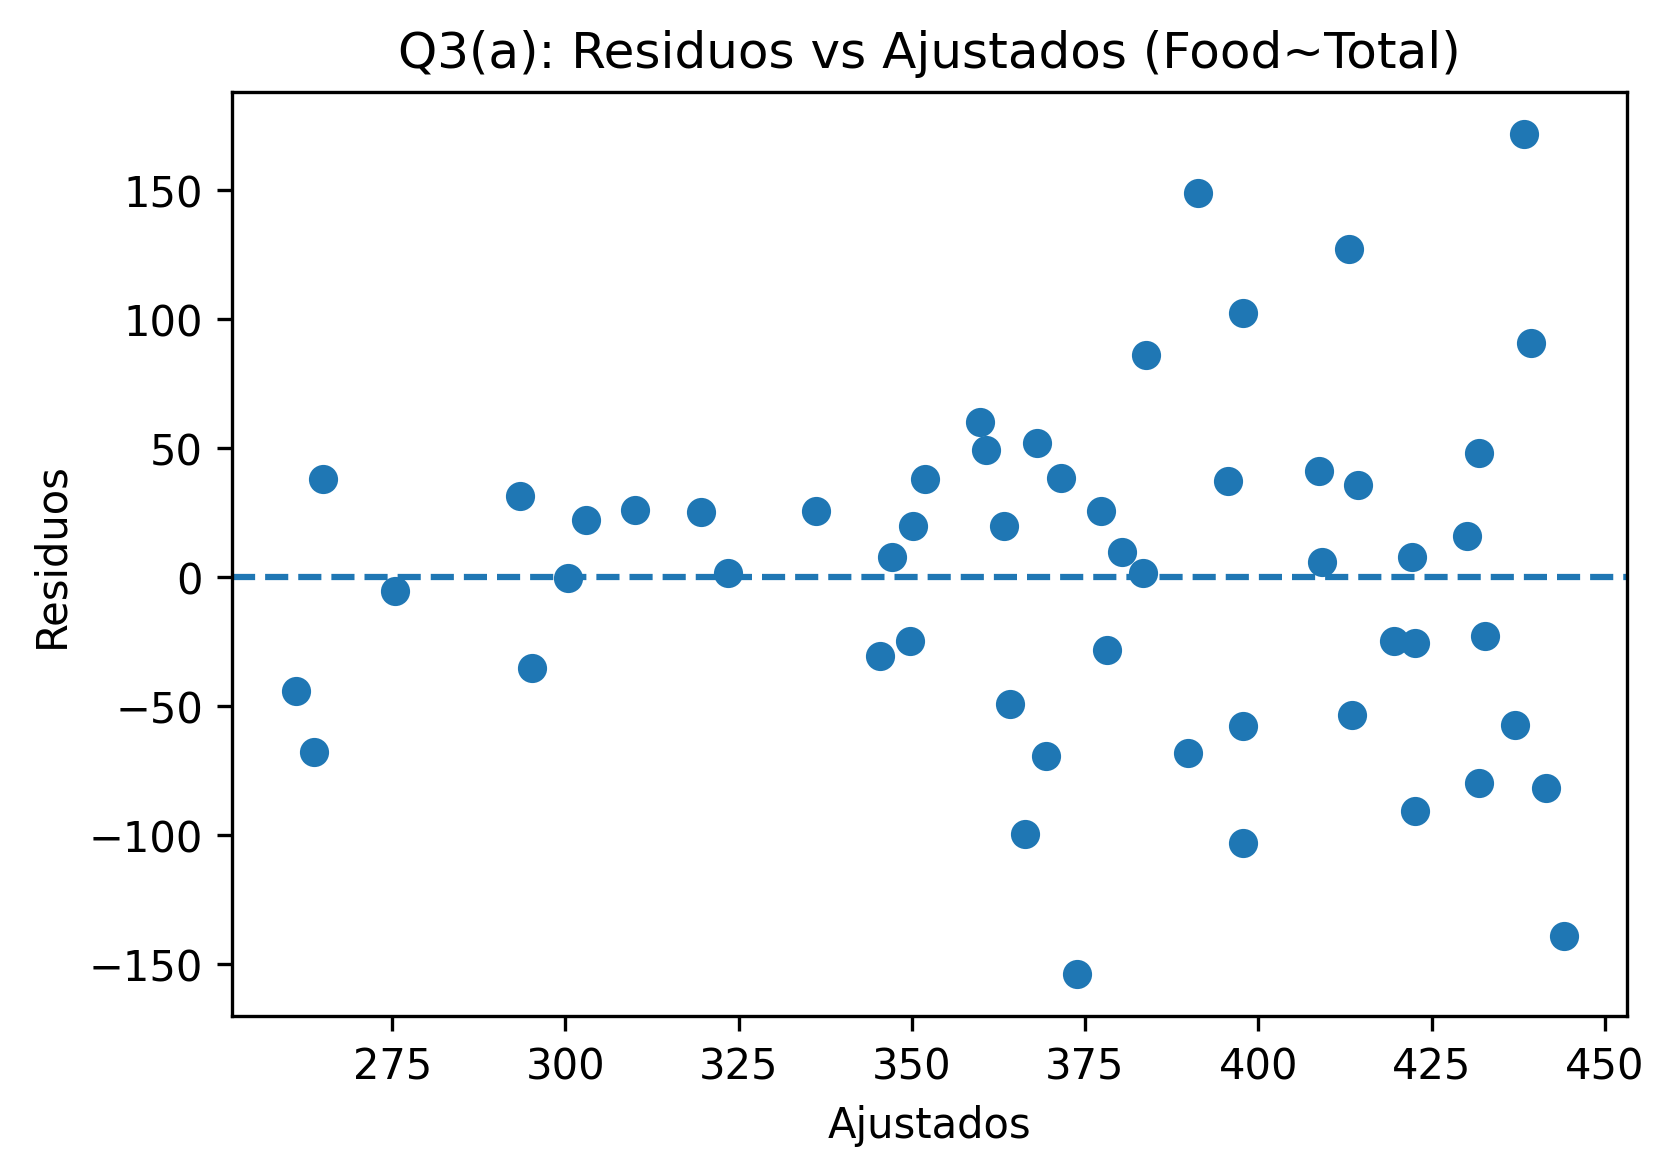
\includegraphics[width=0.7\linewidth]{../plots/python/ex3/q3_a_resid_vs_fitted.png}
            \caption{Q3(a): Residuos vs Ajustados (Food~Total)}
            \label{fig:q3_a_resid}
        \end{figure}
        \newpage
        La normalidad de residuos es razonable (Jarque–Bera $p=0.8792$), según el QQ-plot:
        \begin{figure}[H]
            \centering
            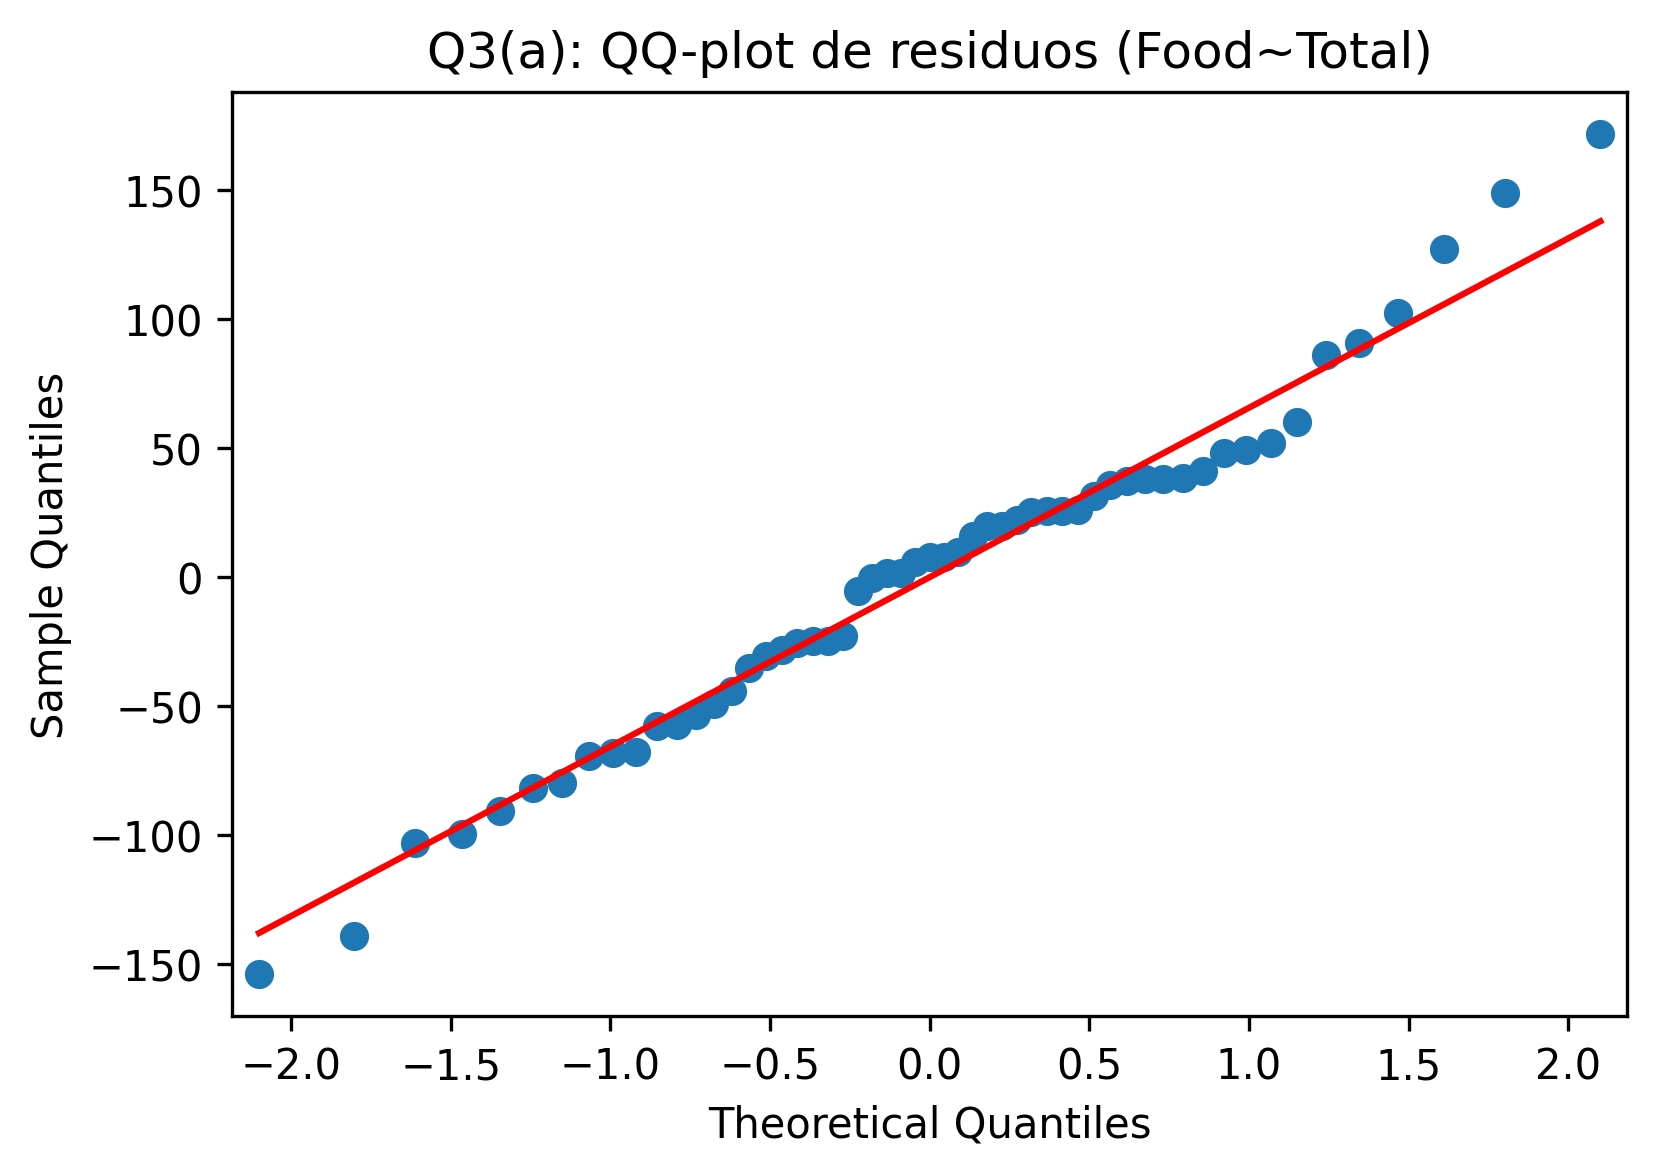
\includegraphics[width=0.7\linewidth]{../plots/python/ex3/q3_a_resid_qqplot.png}
            \caption{Q3(a): QQ-plot de residuos (Food~Total)}
            \label{fig:q3_a_qq}
        \end{figure}
    }
%%%%%%%%%%%%%%%%%%%%%%%%%%%%%%%%%%%%%%%%%%%%%%%%%%%%%%%%%%%%%%%%%%%%%%%%%%%%%%%%%%%%%%%%%%%%%%%%%%%%%%%%%%%%%%
\subsection{Grafique los residuos al cuadrado obtenidos en el inciso a) contra el gasto total y verifique si existe algún patrón sistemático.}
    \textcolor{blue}{
        La relación positiva entre $\widehat{\varepsilon}_i^{\,2}$ y $\text{Total}_i$ es evidente, con mayor dispersión a niveles altos de gasto total.
        \begin{figure}[H]
            \centering
            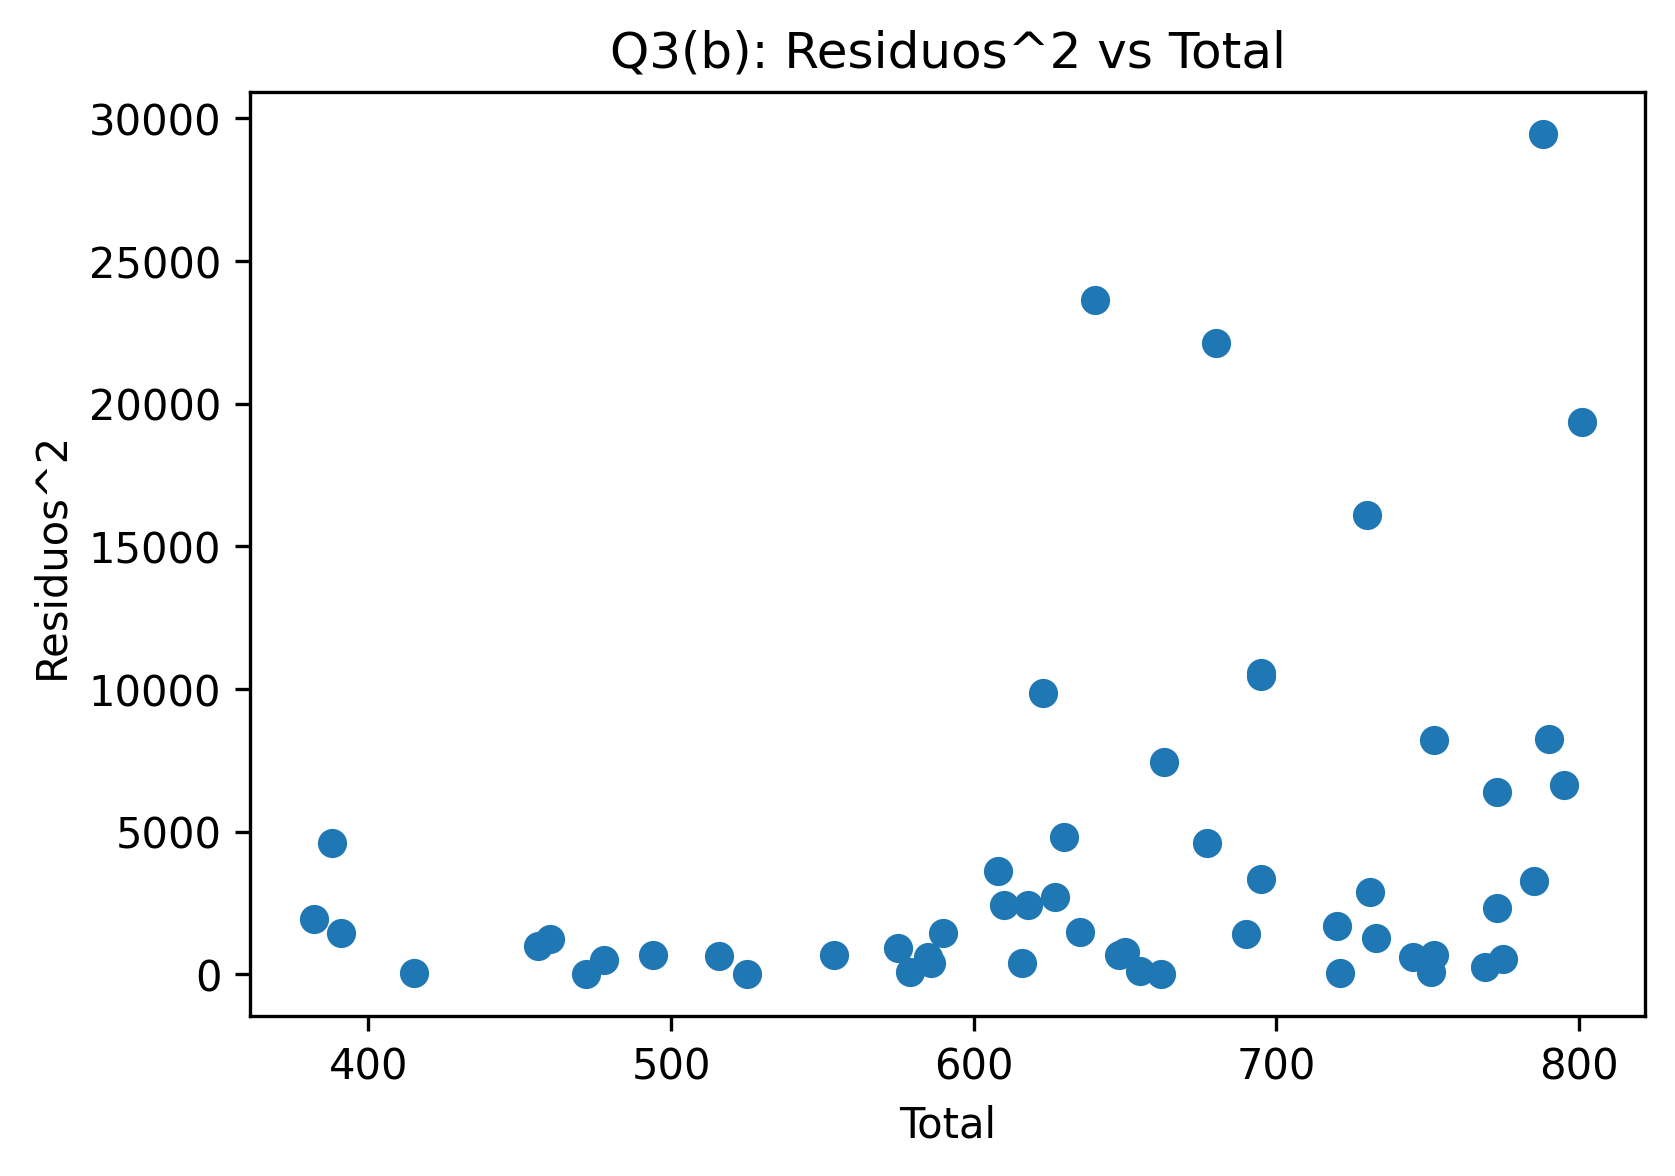
\includegraphics[width=0.7\linewidth]{../plots/python/ex3/q3_b_resid2_vs_total.png}
            \caption{Q3(b): $\widehat{\varepsilon}^{\,2}$ vs. Total}
            \label{fig:q3_b_resid2}
        \end{figure}
        La gráfica sugiere un patrón sistemático de varianza creciente.
    }
%%%%%%%%%%%%%%%%%%%%%%%%%%%%%%%%%%%%%%%%%%%%%%%%%%%%%%%%%%%%%%%%%%%%%%%%%%%%%%%%%%%%%%%%%%%%%%%%%%%%%%%%%%%%%%
\subsection{Si la gráfica del inciso b) sugiere heteroscedasticidad, aplique las pruebas de Park, correlación de orden de Spearman y White para determinar si la sensación respecto de la heteroscedasticidad observada en b) se sustenta con estas pruebas.}
    \textcolor{blue}{
        \textbf{Prueba de Park.} \\
        Modelo probado:
        \begin{equation*}
        \ln(\widehat{\varepsilon}_i^{\,2}) = \alpha + \gamma\,\ln(\text{Total}_i) + u_i.
        \end{equation*}
        Hipótesis: $H_0\!:\ \gamma=0$ (homoscedasticidad) vs. $H_1\!:\ \gamma\neq 0$. \\
        Resultado (Cuadro~\ref{tab:q3c_park}): \(\hat\gamma=3.7032\), $t=2.386$, $p=0.0206$ $\Rightarrow$ \textbf{rechazo de $H_0$}.
        \begin{table}[H]
\centering
\caption{Pregunta 3(c): Prueba de Park (ln(resid\textasciicircum 2)~ln(Total))}
\label{tab:q3c_park}
\begin{tabular}{lrrrrrr}
\rowcolor{blue!10}
\toprule
\rowcolor{blue!20}
\textcolor{blue}{\textbf{Parámetro}} & \textcolor{blue}{\textbf{Coef}} & \textcolor{blue}{\textbf{EE}} & \textcolor{blue}{\textbf{t}} & \textcolor{blue}{\textbf{p-valor}} & \textcolor{blue}{\textbf{IC 2.5\%}} & \textcolor{blue}{\textbf{IC 97.5\%}} \\
\addlinespace
\rowcolor{blue!10}
\textcolor{blue}{Intercept} & \textcolor{blue}{-16.8629} & \textcolor{blue}{10.0014} & \textcolor{blue}{-1.6861} & \textcolor{blue}{0.0977} & \textcolor{blue}{-36.9231} & \textcolor{blue}{3.1974} \\
\rowcolor{blue!10}
\textcolor{blue}{ln\_Total} & \textcolor{blue}{3.7032} & \textcolor{blue}{1.5519} & \textcolor{blue}{2.3863} & \textcolor{blue}{0.0206} & \textcolor{blue}{0.5906} & \textcolor{blue}{6.8159} \\
\bottomrule
\end{tabular}
\end{table}

        \vspace{0.2cm}
        \textbf{Correlación de Spearman.} \\
        Se contrasta la monotonía entre $|\widehat{\varepsilon}_i|$ (o $\widehat{\varepsilon}_i^{\,2}$) y $\text{Total}_i$. Resultado: $\rho=0.3627$, $p=0.0065$ $\Rightarrow$ \textbf{evidencia de heteroscedasticidad}.\\
        \begin{table}[H]
\centering
\caption{Pregunta 3(c): Correlación de Spearman para heteroscedasticidad}
\label{tab:q3c_spearman}
\begin{tabular}{lrr}
\rowcolor{blue!10}
\toprule
\rowcolor{blue!20}
\textcolor{blue}{\textbf{Métrica}} & \textcolor{blue}{\textbf{rho}} & \textcolor{blue}{\textbf{p-valor}} \\
\addlinespace
\rowcolor{blue!10}
\textcolor{blue}{|resid| vs Total} & \textcolor{blue}{0.3627} & \textcolor{blue}{0.0065} \\
\rowcolor{blue!10}
\textcolor{blue}{resid\textasciicircum 2 vs Total} & \textcolor{blue}{0.3627} & \textcolor{blue}{0.0065} \\
\bottomrule
\end{tabular}
\end{table}

        \vspace{0.2cm}
        \textbf{Prueba de White.} \\
        Se reporta el estadístico y su $p$-valor en el Cuadro~\ref{tab:q3c_white}. El contraste compara contra una $\chi^2$ con g.l. correspondientes. Los resultados son consistentes con la presencia de heteroscedasticidad.
        \\
        \begin{table}[H]
\centering
\caption{Pregunta 3(c): Prueba de White (modelo lineal)}
\label{tab:q3c_white}
\begin{tabular}{lrr}
\rowcolor{blue!10}
\toprule
\rowcolor{blue!20}
\textcolor{blue}{\textbf{Prueba}} & \textcolor{blue}{\textbf{Estadístico}} & \textcolor{blue}{\textbf{p-valor}} \\
\addlinespace
\rowcolor{blue!10}
\textcolor{blue}{White} & \textcolor{blue}{7.3745} & \textcolor{blue}{0.0250} \\
\bottomrule
\end{tabular}
\end{table}

        Las tres pruebas respaldan la sospecha de heteroscedasticidad detectada en (a)-(b).
    }
%%%%%%%%%%%%%%%%%%%%%%%%%%%%%%%%%%%%%%%%%%%%%%%%%%%%%%%%%%%%%%%%%%%%%%%%%%%%%%%%%%%%%%%%%%%%%%%%%%%%%%%%%%%%%%
\subsection{Efectúe la regresión del logaritmo del gasto alimentario sobre el logaritmo del gasto total. Si observa heteroscedasticidad en el modelo lineal del inciso a) pero no en el modelo log-log, ¿a qué conclusión llega? Muestre todas las pruebas necesarias.}
    \textcolor{blue}{
        \textbf{Modelo log–log:}
        \begin{equation*}
        \ln(\text{Food}_i) = \beta_0 + \beta_1\,\ln(\text{Total}_i) + \eta_i.
        \end{equation*}
        Estimación OLS (Cuadro~\ref{tab:q3d_loglog_coefs}): \(\hat\beta_1=0.7363\) (\(t=6.100\), $p<0.001$), con \(R^2=0.412\).\\
        \begin{table}[H]
\centering
\caption{Pregunta 3(d): Coeficientes OLS (log-log)}
\label{tab:q3d_loglog_coefs}
\begin{tabular}{lrrrrrr}
\rowcolor{blue!10}
\toprule
\rowcolor{blue!20}
\textcolor{blue}{\textbf{Parámetro}} & \textcolor{blue}{\textbf{Coef}} & \textcolor{blue}{\textbf{EE}} & \textcolor{blue}{\textbf{t}} & \textcolor{blue}{\textbf{p-valor}} & \textcolor{blue}{\textbf{IC 2.5\%}} & \textcolor{blue}{\textbf{IC 97.5\%}} \\
\addlinespace
\rowcolor{blue!10}
\textcolor{blue}{Intercept} & \textcolor{blue}{1.1543} & \textcolor{blue}{0.7780} & \textcolor{blue}{1.4838} & \textcolor{blue}{0.1438} & \textcolor{blue}{-0.4061} & \textcolor{blue}{2.7147} \\
\rowcolor{blue!10}
\textcolor{blue}{ln\_Total} & \textcolor{blue}{0.7363} & \textcolor{blue}{0.1207} & \textcolor{blue}{6.0998} & \textcolor{blue}{0.0000} & \textcolor{blue}{0.4942} & \textcolor{blue}{0.9784} \\
\bottomrule
\end{tabular}
\end{table}

        Los residuos del modelo log–log muestran varianza más estable y mejor normalidad:
        \begin{figure}[H]
            \centering
            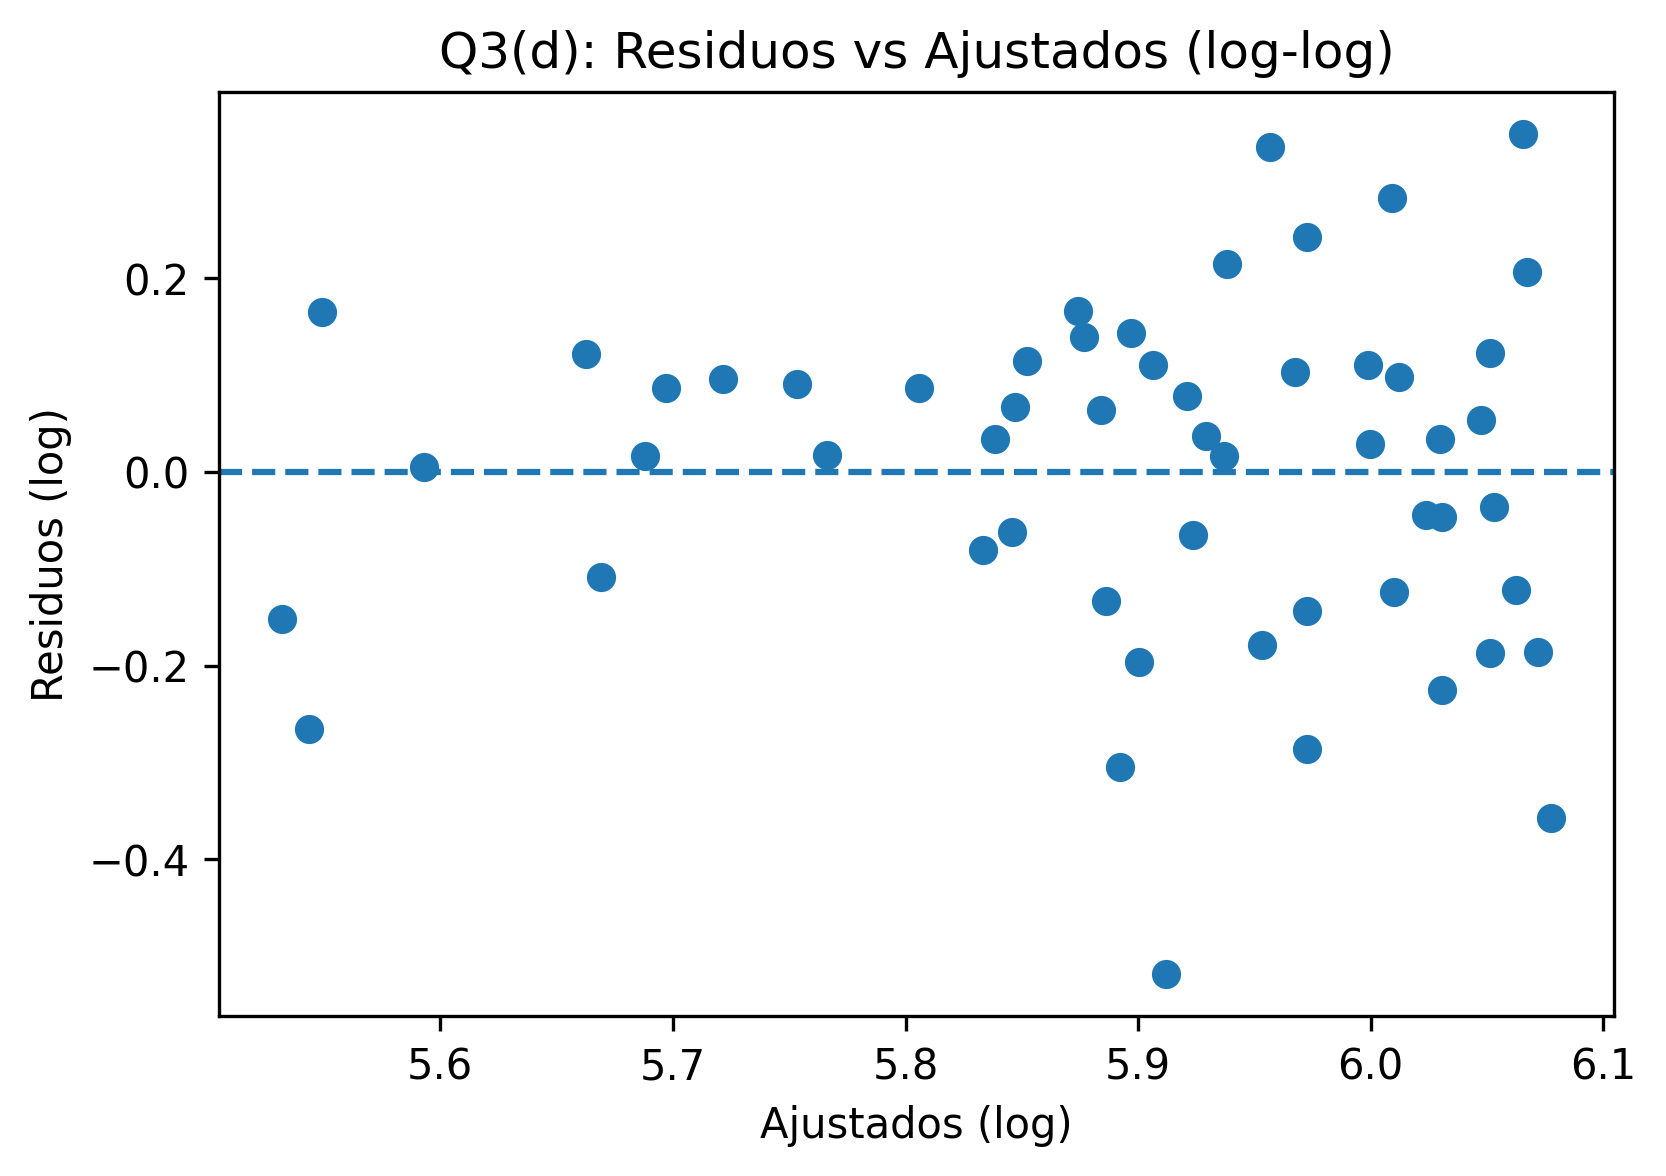
\includegraphics[width=0.7\linewidth]{../plots/python/ex3/q3_d_loglog_resid_vs_fitted.png}
            \caption{Q3(d): Residuos vs Ajustados (log–log)}
            \label{fig:q3_d_resid}
        \end{figure}
        \begin{figure}[H]
            \centering
            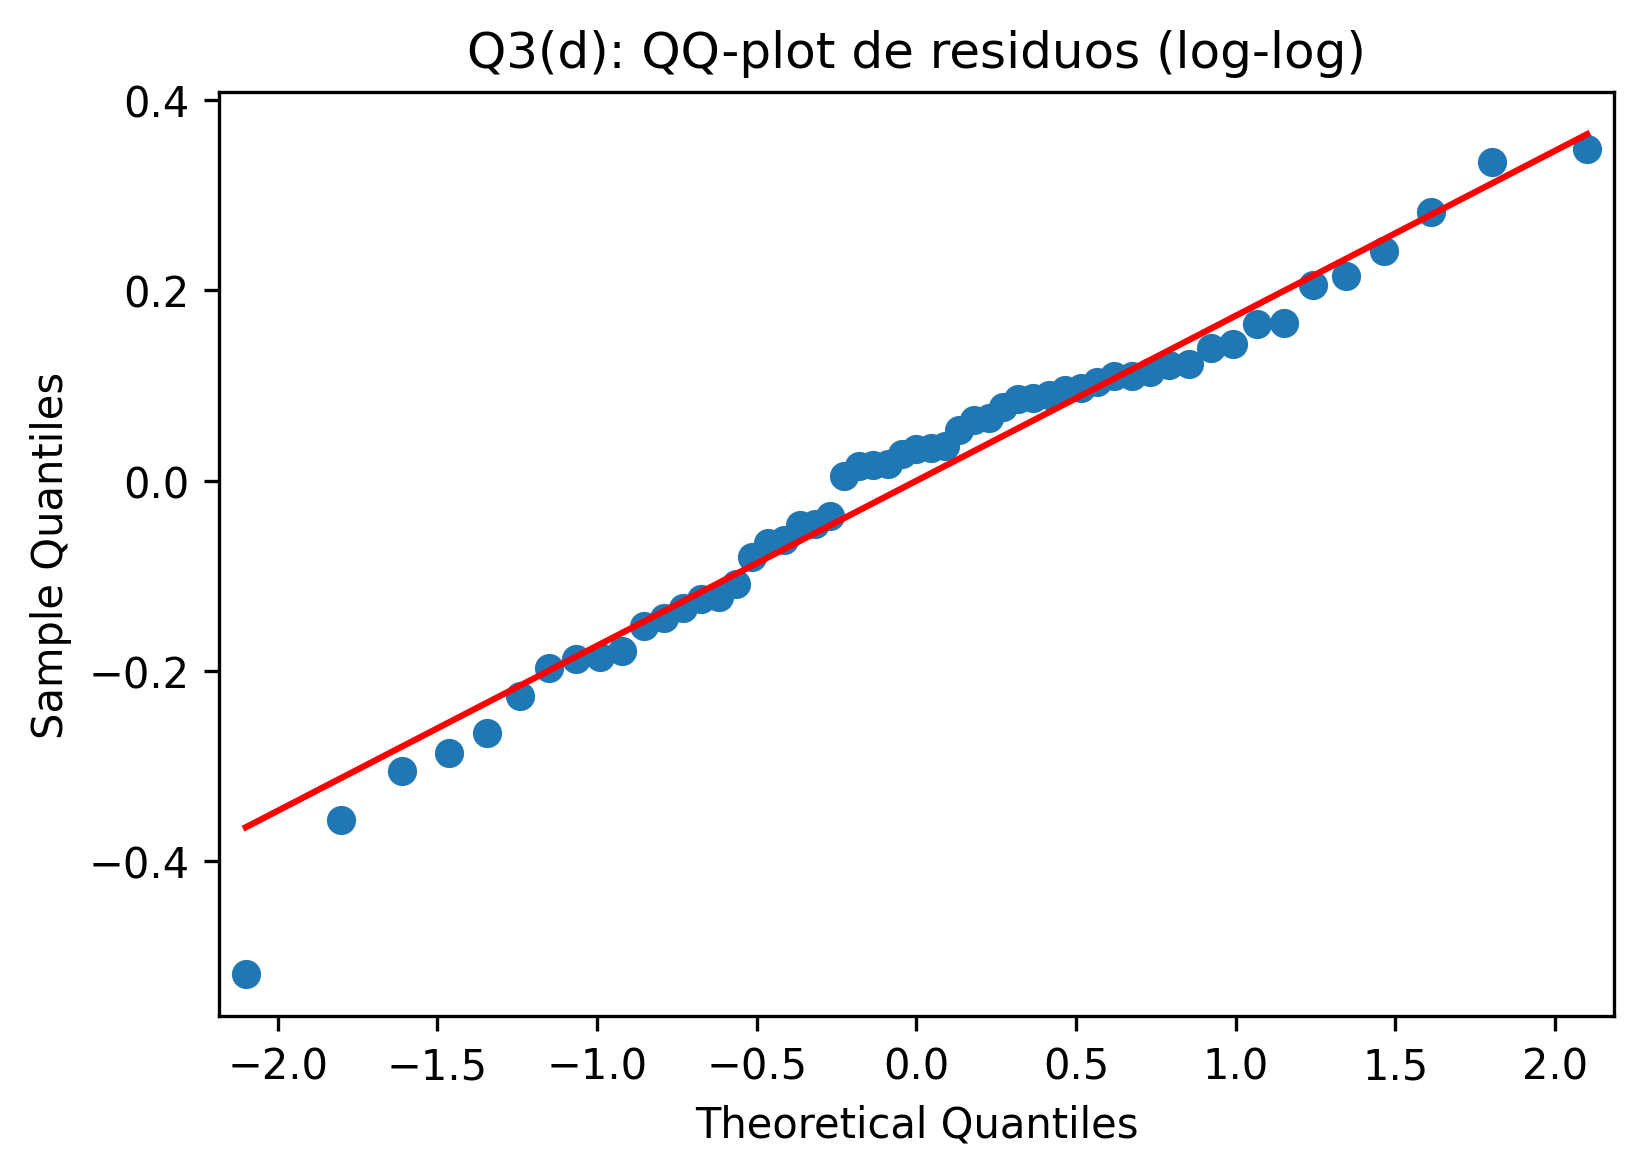
\includegraphics[width=0.7\linewidth]{../plots/python/ex3/q3_d_loglog_resid_qqplot.png}
            \caption{Q3(d): QQ-plot de residuos (log–log)}
            \label{fig:q3_d_qq}
        \end{figure}
        Pruebas (Cuadro~\ref{tab:q3d_loglog_hetero}) indican no rechazar homoscedasticidad en el modelo transformado.
        \\
        \begin{table}[H]
\centering
\caption{Pregunta 3(d): Pruebas de heterocedasticidad (log-log)}
\label{tab:q3d_loglog_hetero}
\begin{tabular}{lr}
\rowcolor{blue!10}
\toprule
\rowcolor{blue!20}
\textcolor{blue}{\textbf{Prueba}} & \textcolor{blue}{\textbf{p-valor}} \\
\addlinespace
\rowcolor{blue!10}
\textcolor{blue}{White} & \textcolor{blue}{0.3600} \\
\rowcolor{blue!10}
\textcolor{blue}{Breusch-Pagan} & \textcolor{blue}{0.2355} \\
\bottomrule
\end{tabular}
\end{table}

        La heteroscedasticidad en el modelo lineal parece deberse a varianza proporcional al nivel de gasto. La transformación logarítmica estabiliza la varianza y mejora los supuestos clásicos, por lo que el modelo log–log es preferible para hacer inferencia.
    }
%%%%%%%%%%%%%%%%%%%%%%%%%%%%%%%%%%%%%%%%%%%%%%%%%%%%%%%%%%%%%%%%%%%%%%%%%%%%%%%%%%%%%%%%%%%%%%%%%%%%%%%%%%%%%%
%%%%%%%%%%%%%%%%%%%%%%%%%%%%%%%%%%%%%%%%%%%%%%%%%%%%%%%%%%%%%%%%%%%%%%%%%%%%%%%%%%%%%%%%%%%%%%%%%%%%%%%%%%%%%%
%%%%%%%%%%%%%%%%%%%%%%%%%%%%%%%%%%%%%%%%%%%%%%%%%%%%%%%%%%%%%%%%%%%%%%%%%%%%%%%%%%%%%%%%%%%%%%%%%%%%%%%%%%%%%%
%%%%%%%%%%%%%%%%%%%%%%%%%%%%%%%%%%%%%%%%%%%%%%%%%%%%%%%%%%%%%%%%%%%%%%%%%%%%%%%%%%%%%%%%%%%%%%%%%%%%%%%%%%%%%%
\section{Pregunta 4}
Establezca si las siguientes afirmaciones son verdaderas o falsas. Justifique brevemente.
%%%%%%%%%%%%%%%%%%%%%%%%%%%%%%%%%%%%%%%%%%%%%%%%%%%%%%%%%%%%%%%%%%%%%%%%%%%%%%%%%%%%%%%%%%%%%%%%%%%%%%%%%%%%%%
\subsection{Cuando hay presencia de autocorrelación, los estimadores de MCO son sesgados e ineficientes.}
\textcolor{blue}{
    \textbf{Falso.} Con $E(u_t\mid X)=0$, los estimadores MCO siguen siendo \emph{insesgados} y consistentes; lo que falla es la eficiencia y la inferencia porque $\mathrm{Var}(\hat\beta)$ ya no es $\sigma^2(X'X)^{-1}$ sino $(X'X)^{-1}X'\Sigma X(X'X)^{-1}$ con $\Sigma\neq\sigma^2 I$. Los errores estándar “convencionales” quedan mal calculados; usar GLS o correcciones tipo Newey--West.
}
%%%%%%%%%%%%%%%%%%%%%%%%%%%%%%%%%%%%%%%%%%%%%%%%%%%%%%%%%%%%%%%%%%%%%%%%%%%%%%%%%%%%%%%%%%%%%%%%%%%%%%%%%%%%%%
\subsection{La prueba DW de Durbin--Watson supone que la varianza del término de error u\_t es homoscedástica.}
\textcolor{blue}{
    \textbf{Verdadero.} El contraste DW se deriva bajo $H_0\!:\ \rho=0$ suponiendo errores homoscedásticos e independientes en ausencia de autocorrelación y sin $y_{t-1}$ como regresor. Heteroscedasticidad o términos dependientes afectan su validez.
}
%%%%%%%%%%%%%%%%%%%%%%%%%%%%%%%%%%%%%%%%%%%%%%%%%%%%%%%%%%%%%%%%%%%%%%%%%%%%%%%%%%%%%%%%%%%%%%%%%%%%%%%%%%%%%%
\subsection{La transformación de primeras diferencias para eliminar la autocorrelación supone que el coeficiente de autocorrelación rho es -1.}
\textcolor{blue}{
    \textbf{Falso.} La \emph{primeras diferencias} corresponde al caso especial de cuasi‑diferenciación cuando $\rho=1$ (no $-1$). Para $u_t=\rho u_{t-1}+\varepsilon_t$, la transformación correcta es $y_t-\rho y_{t-1}$ y $x_t-\rho x_{t-1}$; si $\rho=1$ se reduce a diferenciar.
}
%%%%%%%%%%%%%%%%%%%%%%%%%%%%%%%%%%%%%%%%%%%%%%%%%%%%%%%%%%%%%%%%%%%%%%%%%%%%%%%%%%%%%%%%%%%%%%%%%%%%%%%%%%%%%%
\subsection{Los valores R² de dos modelos, de los cuales uno corresponde a una regresión en primeras diferencias y el otro a una regresión en niveles, no son directamente comparables.}
\textcolor{blue}{
    \textbf{Verdadero.} En primeras diferencias la variable dependiente cambia de escala y varianza, por lo que $TSS$ y, en consecuencia, $R^2=1-SSR/TSS$ se definen sobre magnitudes distintas al modelo en niveles; no son comparables entre especificaciones con dependientes diferentes.
}
%%%%%%%%%%%%%%%%%%%%%%%%%%%%%%%%%%%%%%%%%%%%%%%%%%%%%%%%%%%%%%%%%%%%%%%%%%%%%%%%%%%%%%%%%%%%%%%%%%%%%%%%%%%%%%
\subsection{Un DW de Durbin--Watson significativo no necesariamente denota autocorrelación de primer orden.}
\textcolor{blue}{
    \textbf{Verdadero.} Un DW extremo rechaza $H_0:\rho=0$, pero la causa puede ser autocorrelación de orden superior, estacionalidad, omisiones o mala especificación. El test no identifica que el proceso sea estrictamente AR(1).
}
%%%%%%%%%%%%%%%%%%%%%%%%%%%%%%%%%%%%%%%%%%%%%%%%%%%%%%%%%%%%%%%%%%%%%%%%%%%%%%%%%%%%%%%%%%%%%%%%%%%%%%%%%%%%%%
\subsection{En presencia de autocorrelación, las varianzas calculadas convencionalmente y los errores estándar de los valores pronosticados son ineficientes.}
\textcolor{blue}{
    \textbf{Verdadero.} Con $\Sigma\neq\sigma^2 I$, los estimadores de varianza “convencionales” son inválidos o inconsistentes y tienden a subestimar la incertidumbre; por tanto los errores estándar y bandas de predicción basadas en ellos no son confiables. Use GLS o correcciones robustas (HAC/Newey–West).
}
%%%%%%%%%%%%%%%%%%%%%%%%%%%%%%%%%%%%%%%%%%%%%%%%%%%%%%%%%%%%%%%%%%%%%%%%%%%%%%%%%%%%%%%%%%%%%%%%%%%%%%%%%%%%%%
\subsection{La exclusión de una o varias variables importantes de un modelo de regresión puede producir un valor DW significativo.}
\textcolor{blue}{
    \textbf{Verdadero.} Omitir variables relevantes con persistencia temporal hace que el término de error incluya un componente serialmente correlacionado ($w_t$), induciendo $\rho\neq0$ y, por tanto, un estadístico DW significativo aunque el verdadero error estructural fuese no correlacionado.
}
%%%%%%%%%%%%%%%%%%%%%%%%%%%%%%%%%%%%%%%%%%%%%%%%%%%%%%%%%%%%%%%%%%%%%%%%%%%%%%%%%%%%%%%%%%%%%%%%%%%%%%%%%%%%%%
%%%%%%%%%%%%%%%%%%%%%%%%%%%%%%%%%%%%%%%%%%%%%%%%%%%%%%%%%%%%%%%%%%%%%%%%%%%%%%%%%%%%%%%%%%%%%%%%%%%%%%%%%%%%%
\section{Pregunta 5}
Con una muestra de 50 observaciones y 4 variables explicativas, ¿qué puede decir sobre autocorrelación si
%%%%%%%%%%%%%%%%%%%%%%%%%%%%%%%%%%%%%%%%%%%%%%%%%%%%%%%%%%%%%%%%%%%%%%%%%%%%%%%%%%%%%%%%%%%%%%%%%%%%%%%%%%%%%%
\subsection{a) DW=1.05}
\textcolor{blue}{
\textbf{Evidencia de autocorrelación positiva.} Regla aproximada: $\hat\rho\approx1-\tfrac{DW}{2}=1-0.525=0.475$. Con tablas DW (n=50, k=4), valores tan bajos suelen caer por debajo de $d_L$ → rechazar $H_0:\rho=0$ a favor de $\rho>0$.
}
%%%%%%%%%%%%%%%%%%%%%%%%%%%%%%%%%%%%%%%%%%%%%%%%%%%%%%%%%%%%%%%%%%%%%%%%%%%%%%%%%%%%%%%%%%%%%%%%%%%%%%%%%%%%%%
\subsection{b) DW=1.40}
\textcolor{blue}{
\textbf{Autocorrelación positiva moderada (posible) o zona indeterminada.} Aproximación: $\hat\rho\approx1-0.70=0.30$. Sin tablas exactas, es probable que $DW$ esté entre $d_L$ y $d_U$ → conclusión formal: \emph{indeterminada} al 5\%; indicios de $\rho>0$.
}
%%%%%%%%%%%%%%%%%%%%%%%%%%%%%%%%%%%%%%%%%%%%%%%%%%%%%%%%%%%%%%%%%%%%%%%%%%%%%%%%%%%%%%%%%%%%%%%%%%%%%%%%%%%%%%
\subsection{c) DW=2.50}
\textcolor{blue}{
\textbf{Conclusión indeterminada al 5\% (posible $\rho<0$, no concluyente).} Aproximación: $\hat\rho\approx1-1.25=-0.25$. Para probarr $4-\textit{DW}$ con $d_L$ y $d_U$: aquí $4-2.50=1.50$ y, con $n=50$, $k=4$, suele cumplirse $d_L<1.50<d_U$ $\Rightarrow$ \emph{zona indeterminada}. No se rechaza ni se acepta $H_0:\rho=0$.
}
%%%%%%%%%%%%%%%%%%%%%%%%%%%%%%%%%%%%%%%%%%%%%%%%%%%%%%%%%%%%%%%%%%%%%%%%%%%%%%%%%%%%%%%%%%%%%%%%%%%%%%%%%%%%%%
\subsection{d) DW=3.97}
\textcolor{blue}{
\textbf{Autocorrelación negativa muy fuerte.} $\hat\rho\approx1-\tfrac{3.97}{2}=1-1.985=-0.985$ (cercano a $-1$). Normalmente $DW>4-d_L$ → rechazar $H_0:\rho=0$ a favor de $\rho<0$.
}
%%%%%%%%%%%%%%%%%%%%%%%%%%%%%%%%%%%%%%%%%%%%%%%%%%%%%%%%%%%%%%%%%%%%%%%%%%%%%%%%%%%%%%%%%%%%%%%%%%%%%%%%%%%%%%
%%%%%%%%%%%%%%%%%%%%%%%%%%%%%%%%%%%%%%%%%%%%%%%%%%%%%%%%%%%%%%%%%%%%%%%%%%%%%%%%%%%%%%%%%%%%%%%%%%%%%%%%%%%%%%
\section{Pregunta 6}
Establezca las circunstancias en que sería adecuado cada uno de los siguientes métodos de estimación del coeficiente de autocorrelación de primer orden $\rho$:

\subsection{a) Regresión de primeras diferencias}
\textcolor{blue}{
\textbf{Adecuada cuando} la autocorrelación es de primer orden \emph{positiva} y elevada ($0<\rho<1$, típicamente $\rho\approx1$) y se desea eliminar la persistencia. La cuasi‑diferenciación $y_t-\rho y_{t-1}$ se reduce a \\ \emph{primeras diferencias} si $\rho=1$. Útil con tendencias suaves o nivel casi integrado, sin $y_{t-1}$ como regresor y con $T$ moderado–grande (la pérdida de una observación no es crítica). No es recomendable si $\rho$ es negativo o pequeño.
}

\subsection{b) Regresión de promedios móviles}
\textcolor{blue}{
\textbf{Útil como heurística cuando} la autocorrelación de primer orden es \emph{negativa} ($\rho\approx-1$) y los errores alternan de signo ("serrucho"). Promediar observaciones sucesivas (p.ej. $\tfrac{1}{2}(y_t+y_{t-1})$ y $\tfrac{1}{2}(x_t+x_{t-1})$) puede atenuar esa alternancia; sin embargo, \emph{no es el método estándar para estimar} $\rho$. En aplicaciones formales se prefiere \textbf{GLS} tipo \emph{Cochrane--Orcutt} o \emph{Prais--Winsten} estimando $\rho<0$, o bien revisar si hay \emph{sobre‑diferenciación} que induzca $\rho$ negativo. No es adecuado para $\rho>0$ ni para tendencias marcadas.
}
%%%%%%%%%%%%%%%%%%%%%%%%%%%%%%%%%%%%%%%%%%%%%%%%%%%%%%%%%%%%%%%%%%%%%%%%%%%%%%%%%%%%%%%%%%%%%%%%%%%%%%%%%%%%%%
%%%%%%%%%%%%%%%%%%%%%%%%%%%%%%%%%%%%%%%%%%%%%%%%%%%%%%%%%%%%%%%%%%%%%%%%%%%%%%%%%%%%%%%%%%%%%%%%%%%%%%%%%%%%%%
%%%%%%%%%%%%%%%%%%%%%%%%%%%%%%%%%%%%%%%%%%%%%%%%%%%%%%%%%%%%%%%%%%%%%%%%%%%%%%%%%%%%%%%%%%%%%%%%%%%%%%%%%%%%%%
\section{Pregunta 7}
Consulte los datos sobre la industria del cobre de la tabla 12.7.

Con base en esta información, estime el siguiente modelo de regresión:
\begin{equation*}
\ln C_t 
= \beta_1 
+ \beta_2\,\ln I_t 
+ \beta_3\,\ln L_t 
+ \beta_4\,\ln H_t 
+ \beta_5\,\ln A_t 
+ u_t.
\end{equation*}

\subsection{a) Interprete los resultados.}
    \textcolor{blue}{
        \textbf{Modelo log–log (elasticidades).} Los coeficientes se interpretan como elasticidades de $C$ respecto a cada insumo:\\
        \begin{itemize}
            \item $\widehat{\beta}_2=0.468$ (\textit{Inversión}): un 1\% más de $I$ se asocia con \(\approx 0.47\%\) más de $C$ ($t=2.82$, $p=0.009$).
            \item $\widehat{\beta}_3=0.279$ (\textit{Trabajo} $L$): efecto positivo y significativo ($t=2.44$, $p=0.022$).
            \item $\widehat{\beta}_4=-0.005$ (\textit{Horas} $H$): no significativo ($p=0.972$); no hay evidencia de efecto marginal de $H$ ceteris paribus.
            \item $\widehat{\beta}_5=0.441$ (\textit{A}): efecto positivo y significativo ($t=4.15$, $p<0.001$).
        \end{itemize}
        Ajuste global alto: $R^2=0.936$ ($R^2_{\text{aj}}=0.926$) y $F=91.5$ ($p<10^{-13}$). Normalidad de residuos consistente con Jarque–Bera ($p=0.736$).\\
        \begin{table}
\caption{Resultados OLS para $\ln C_t$ con regresores $\ln I_t, \ln L_t, \ln H_t, \ln A_t$. Errores estándar entre paréntesis.}
\label{tab:q7_a}
\begin{tabular}{lrrrr}
\toprule
Parámetro & Coef. & EE & t & p-valor \\
\midrule
const & -1.5004 & 1.0030 & -1.4959 & 0.1472 \\
lnI & 0.4675 & 0.1660 & 2.8165 & 0.0093 \\
lnL & 0.2794 & 0.1147 & 2.4357 & 0.0223 \\
lnH & -0.0052 & 0.1429 & -0.0360 & 0.9715 \\
lnA & 0.4414 & 0.1065 & 4.1447 & 0.0003 \\
R^2 & 0.9361 & NaN & NaN & NaN \\
R^2 ajustado & 0.9259 & NaN & NaN & NaN \\
N & 30.0000 & NaN & NaN & NaN \\
\bottomrule
\end{tabular}
\end{table}

    }

    \newpage
    \subsection{b) Obtenga los residuos y los residuos estandarizados de la regresión anterior y gráfiquelos. ¿Qué opina sobre la presencia de autocorrelación en estos residuos?}
    \textcolor{blue}{
    \begin{figure}[H]
        \centering
        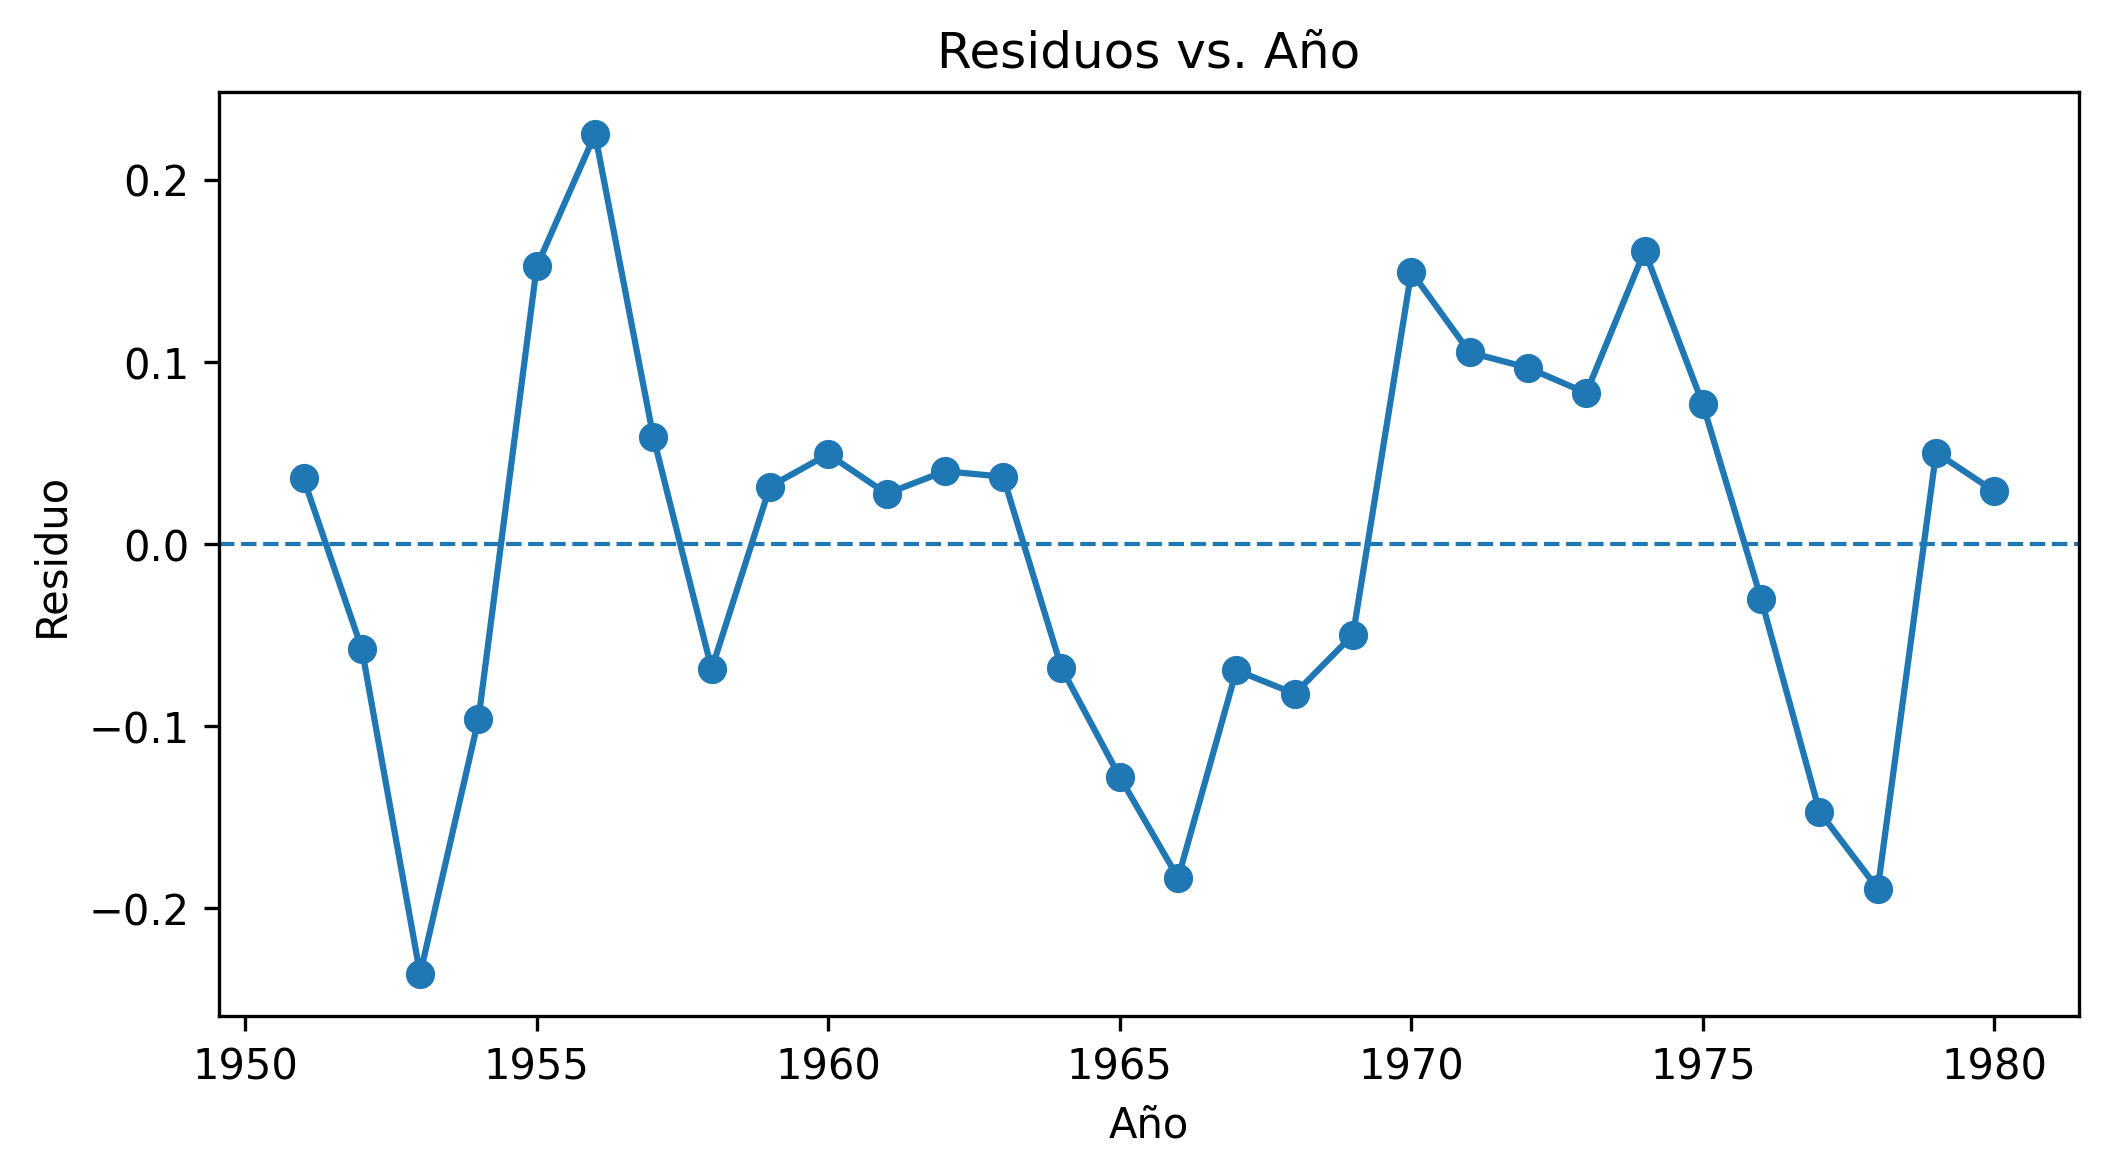
\includegraphics[width=0.9\linewidth]{../plots/python/ex7/ex7_residuos_vs_time.png}
        \caption{Residuos vs. tiempo}
    \end{figure}
    \begin{figure}[H]
        \centering
        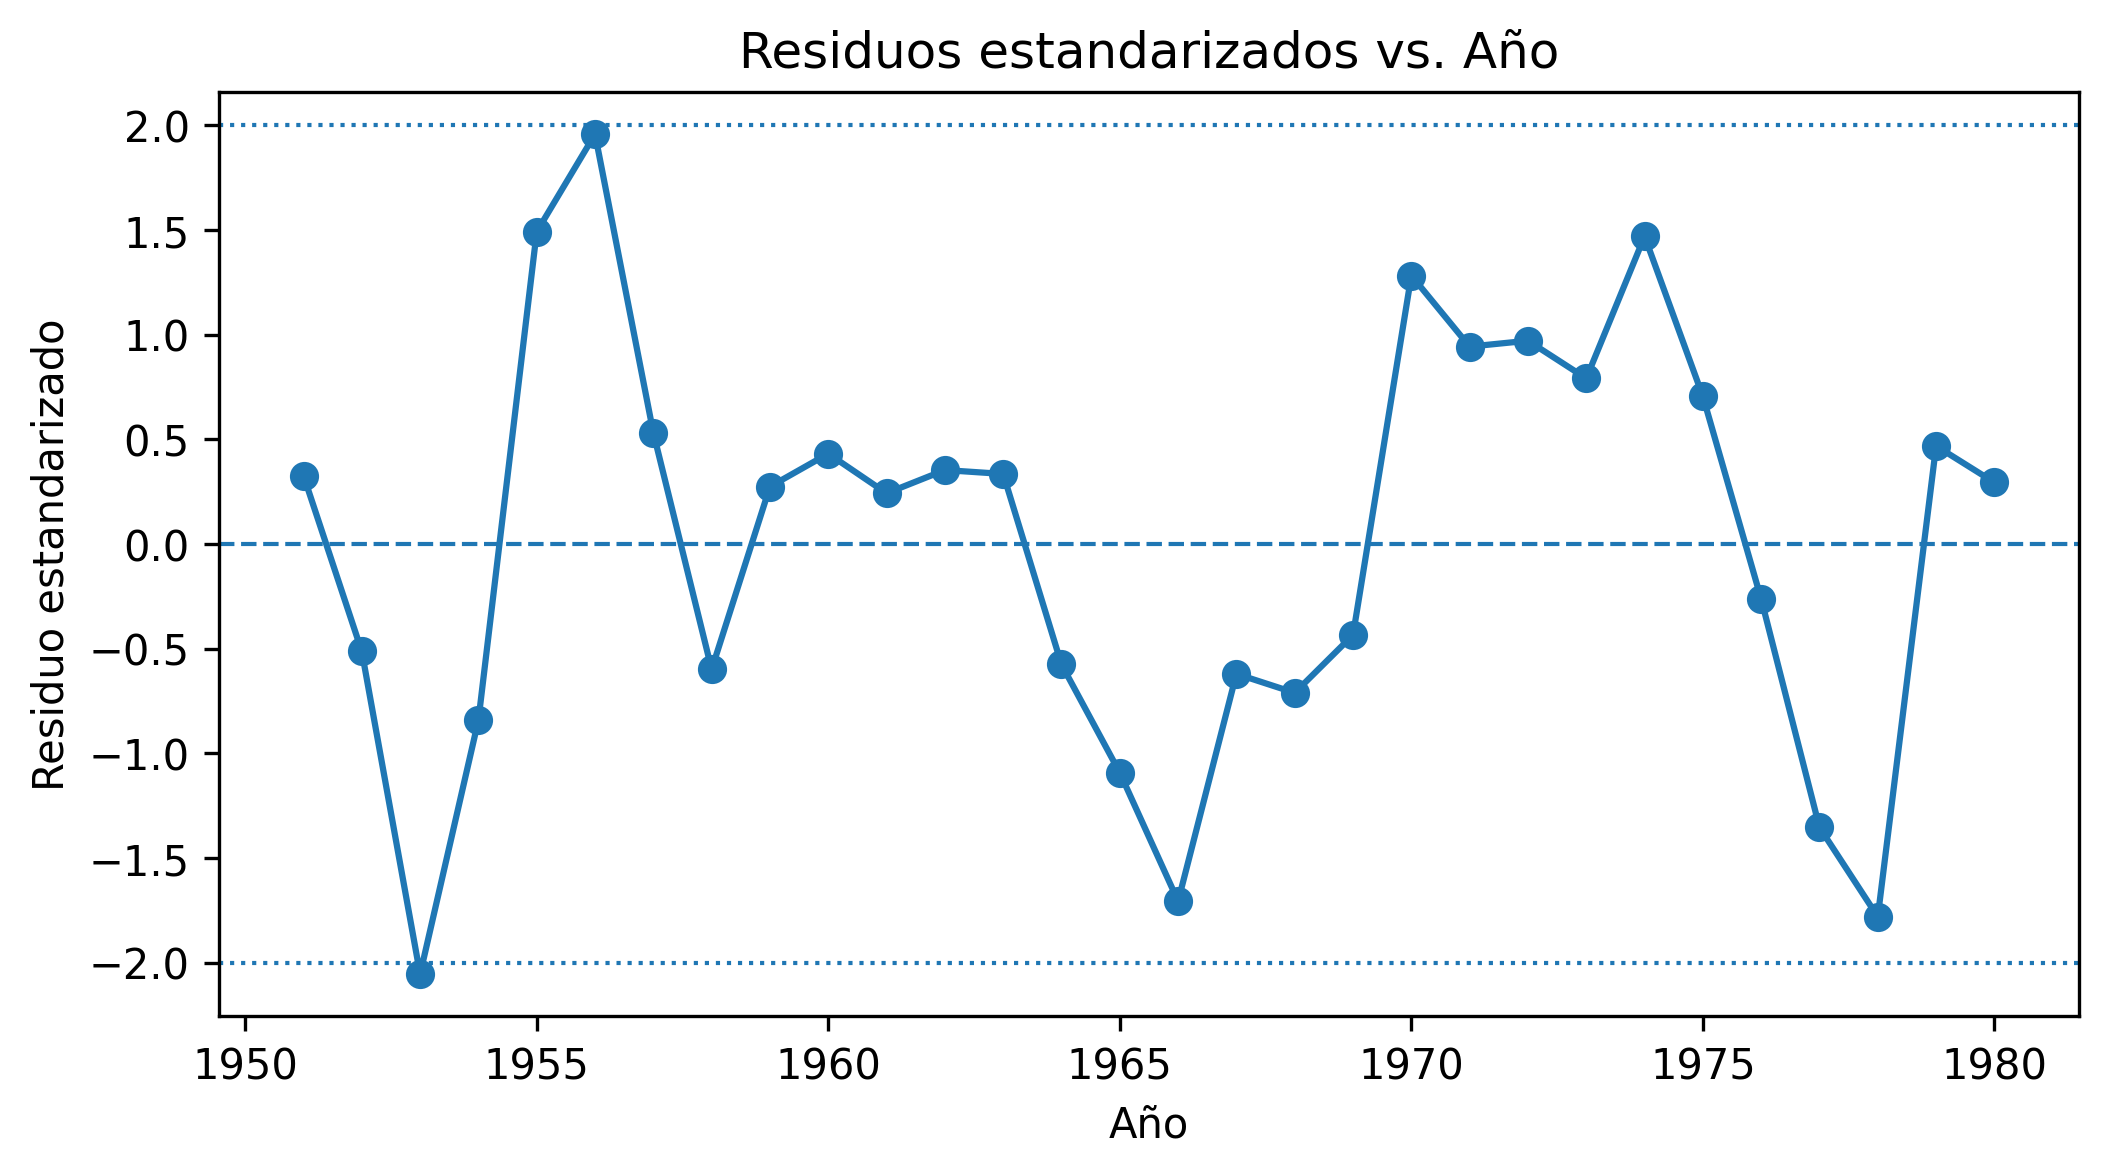
\includegraphics[width=0.9\linewidth]{../plots/python/ex7/ex7_stdres_vs_time.png}
        \caption{Residuos estandarizados vs. tiempo}
    \end{figure}
    \begin{figure}[H]
        \centering
        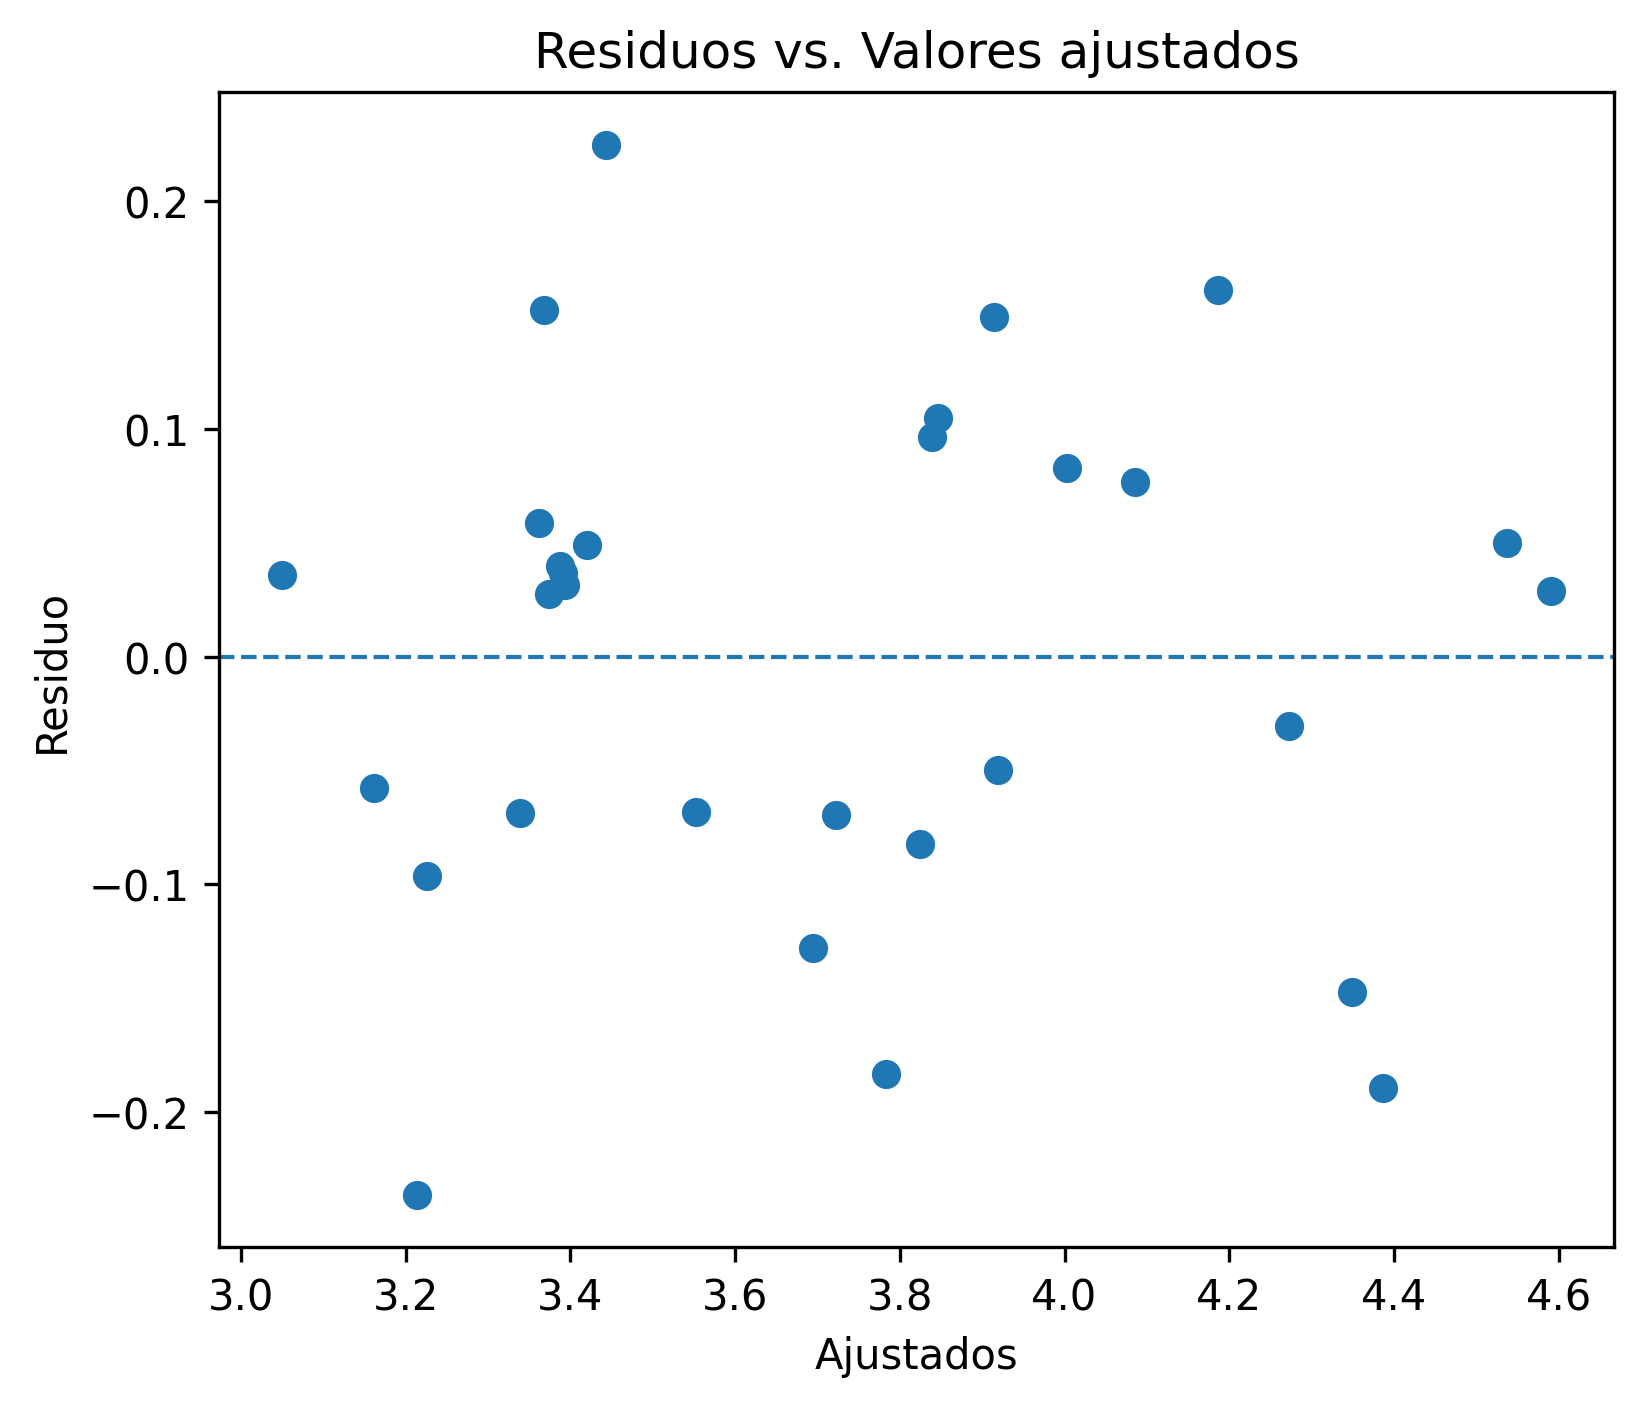
\includegraphics[width=0.55\linewidth]{../plots/python/ex7/ex7_residuos_vs_fitted.png}
        \caption{Residuos vs. ajustados}
    \end{figure}
    \begin{figure}[H]
        \centering
        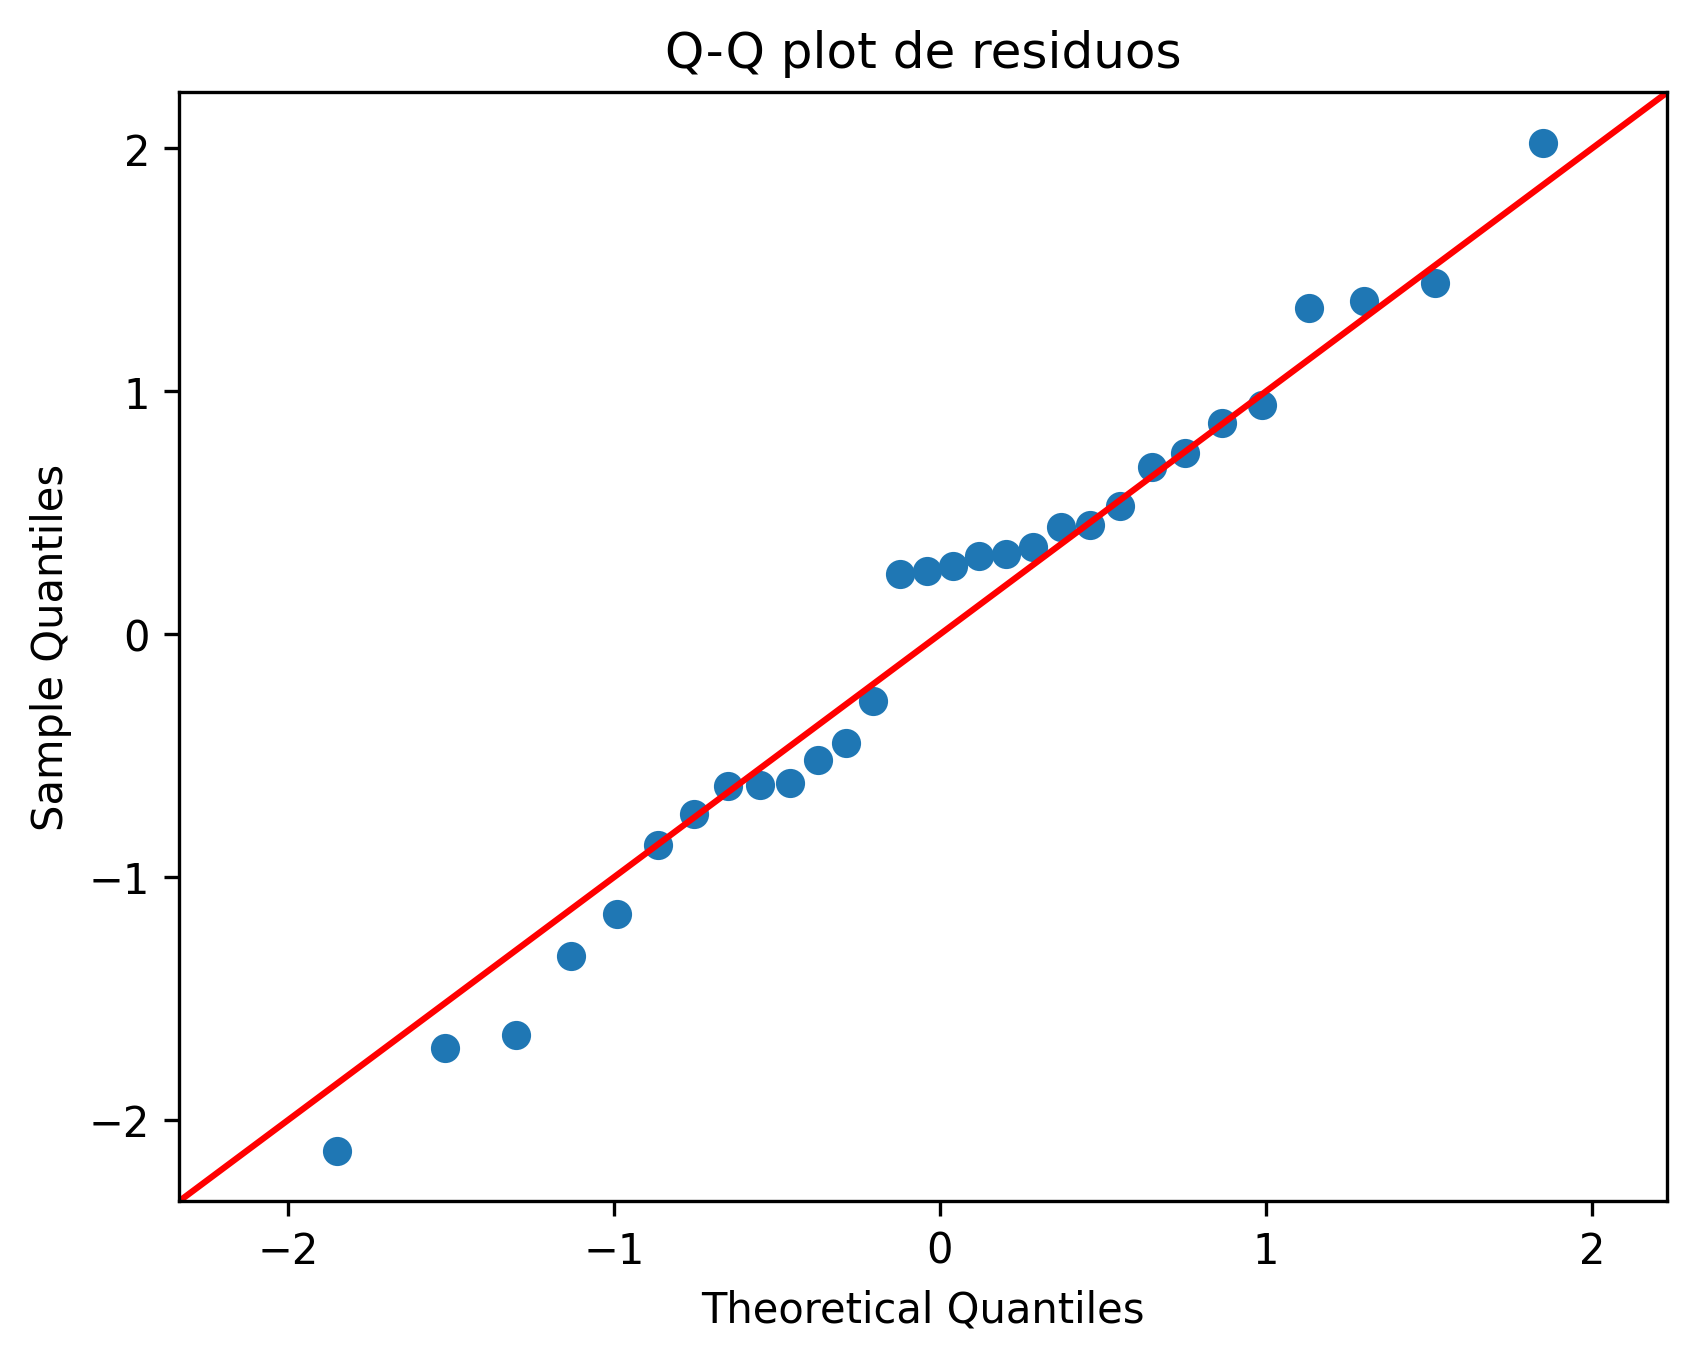
\includegraphics[width=0.55\linewidth]{../plots/python/ex7/ex7_qqplot_residuos.png}
        \caption{QQ-plot de residuos}
    \end{figure}
    Los residuos muestran rachas persistentes (bloques positivos/negativos), lo que sugiere \textbf{autocorrelación positiva}. La nube residuos–ajustados no muestra patrón de abanico marcado (heteroscedasticidad no evidente). El QQ-plot es cercano a la diagonal (normalidad aceptable).
    }

    \subsection{c) Estime el estadístico \texorpdfstring{$DW$}{DW} de Durbin--Watson y comente sobre la naturaleza de la autocorrelación presente en los datos.}
    \textcolor{blue}{
    \textbf{Durbin–Watson.} $DW=0.9549$. Con $n=30$ y $k=4$, un valor tan bajo cae típicamente por debajo de $d_L$ $\Rightarrow$ \textbf{rechazo de $H_0:\rho=0$ a favor de autocorrelación positiva de primer orden}. Esto concuerda con: (i) el diagrama $u_t$ vs. $u_{t-1}$ con pendiente positiva y (ii) la ACF con barra significativa en el rezago 1.\\
    \begin{figure}[H]
        \centering
        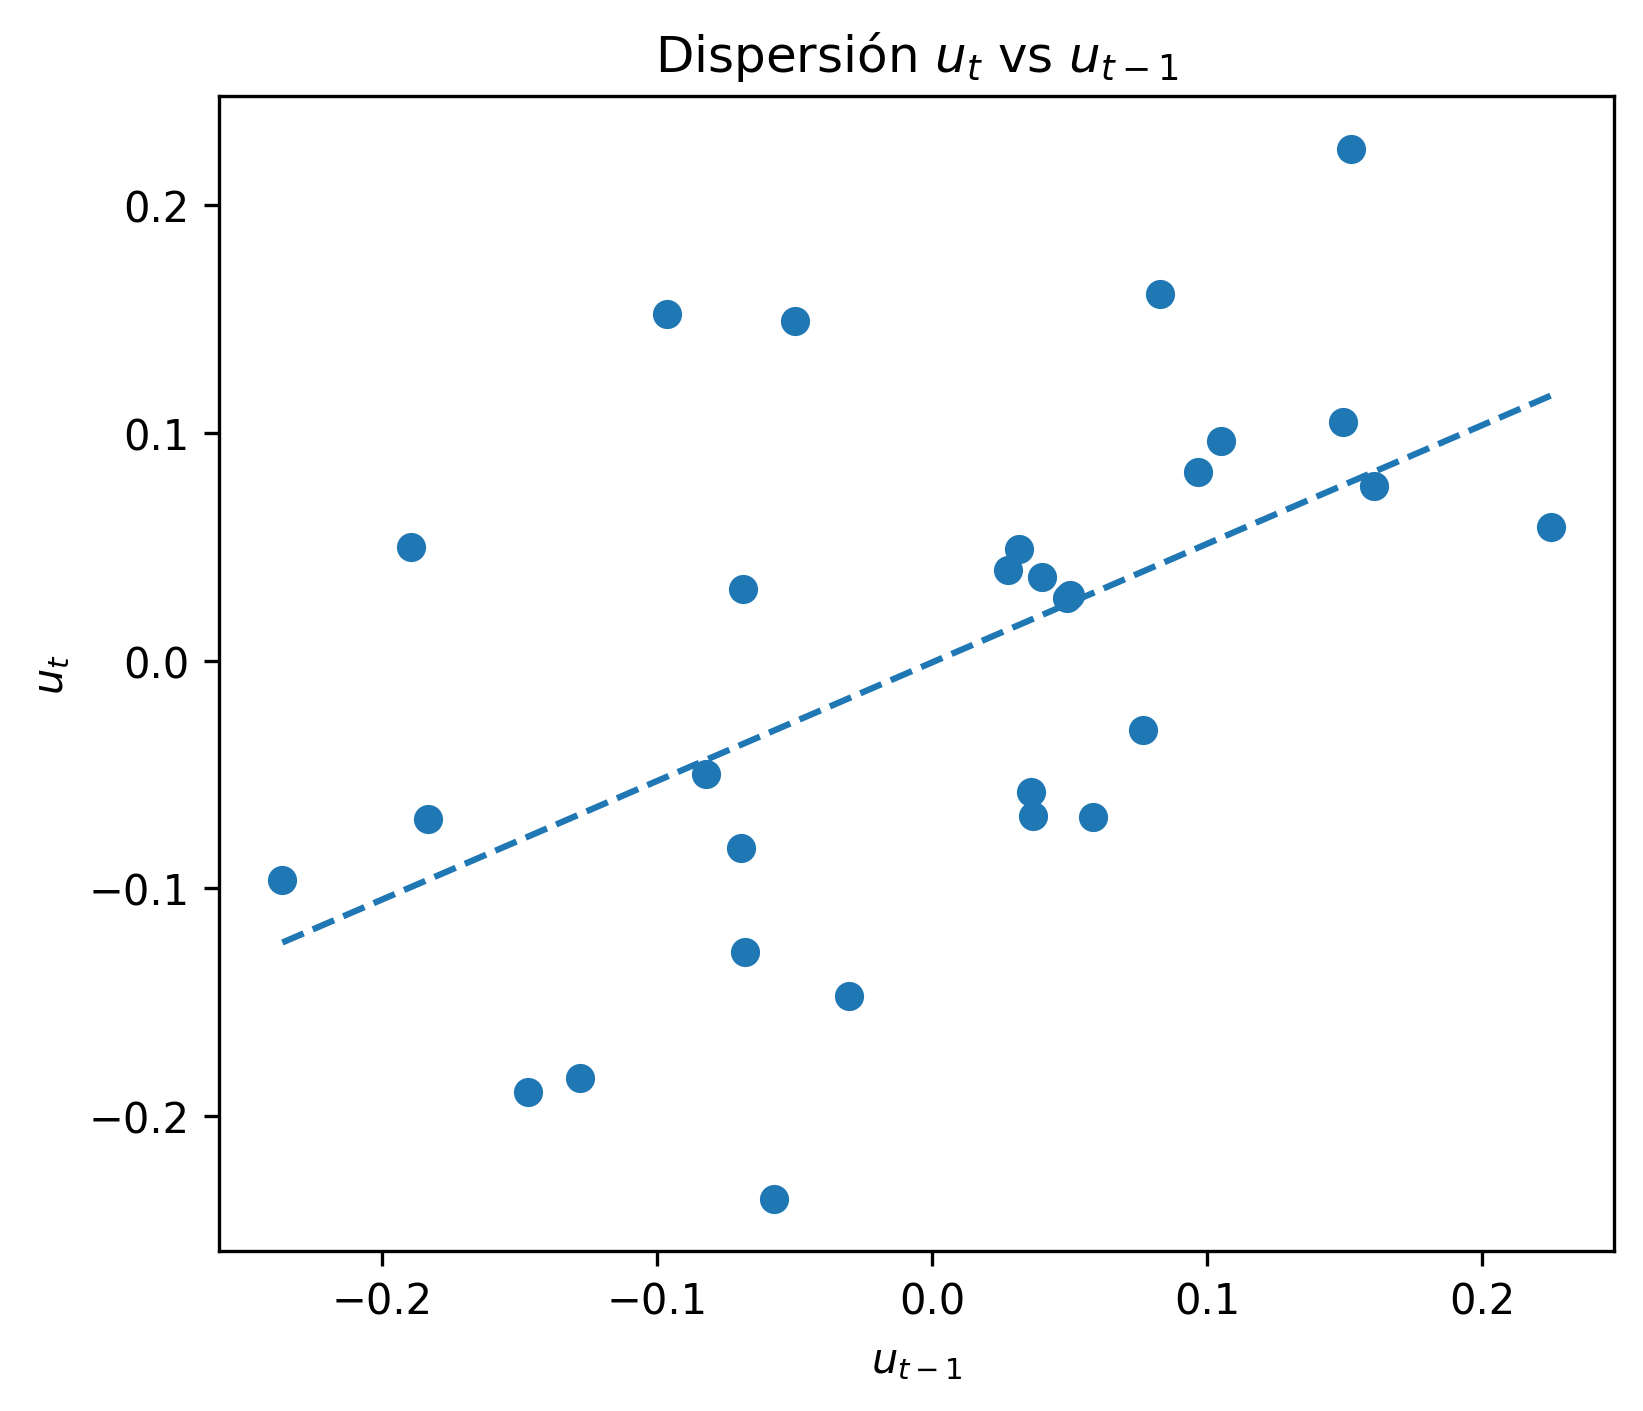
\includegraphics[width=0.55\linewidth]{../plots/python/ex7/ex7_scatter_resid_lag.png}
        \caption{Dispersión $u_t$ vs. $u_{t-1}$}
    \end{figure}
    }

    \subsection{d) Realice las pruebas gráficas de autocorrelación de los errores poblacionales.}
    \textcolor{blue}{
    \begin{figure}[H]
        \centering
        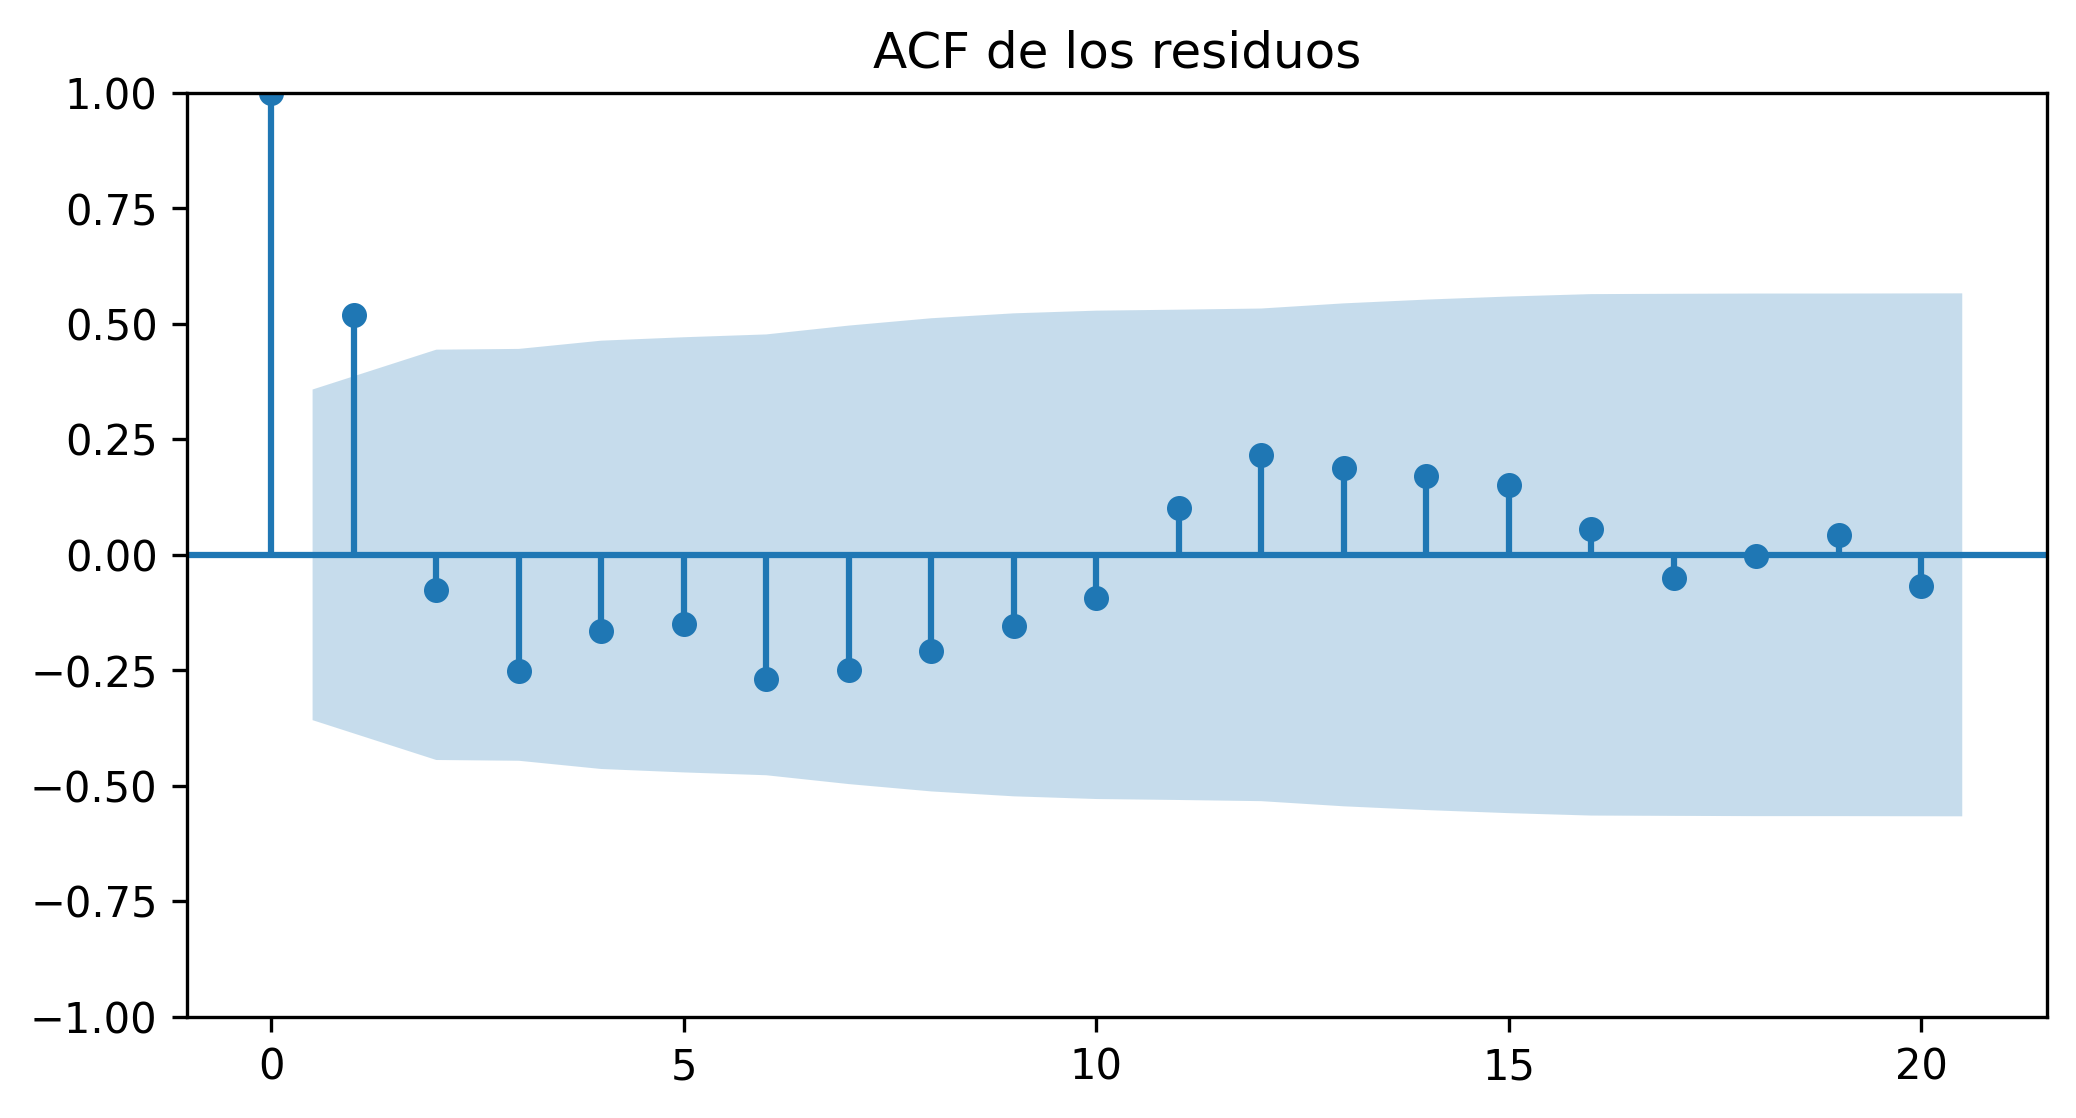
\includegraphics[width=0.95\linewidth]{../plots/python/ex7/ex7_acf_residuos.png}
        \caption{Función de autocorrelación (ACF) de los residuos}
    \end{figure}
    La ACF exhibe una barra positiva y significativa en $\ell=1$ y decaimiento posterior, consistente con un proceso \textbf{AR(1) con $\rho>0$}. En conjunto con $DW<2$, la evidencia apunta a autocorrelación positiva en los errores.
    }
%%
%%%%%%%%%%%%%%%%%%%%%%%%%%%%%%%%%%%%%%%%%%%%%%%%%%%%%%%%%%%%%%%%%%%%%%%%%%%%%%%%%%%%%%%%%%%%%%%%%%%%%%%%%%%%%%
%%%%%%%%%%%%%%%%%%%%%%%%%%%%%%%%%%%%%%%%%%%%%%%%%%%%%%%%%%%%%%%%%%%%%%%%%%%%%%%%%%%%%%%%%%%%%%%%%%%%%%%%%%%%%%
\section{Pregunta 8}
Con los datos proporcionados en la tabla 12.9, estime el modelo
\begin{equation*}
Y_t = \beta_1 + \beta_2 X_t + u_t,
\end{equation*}
\noindent donde $Y$ son inventarios y $X$ ventas, ambas medidas en miles de millones de dólares.

\subsection{a) Estime la regresión anterior.}
\textcolor{blue}{Estimamos
\begin{equation*}
Y_t = \beta_1 + \beta_2 X_t + u_t,\qquad t=1950,\dots,1990.
\end{equation*}
\begin{table}
\caption{Estadísticos descriptivos de ventas, inventarios y razón inventarios/ventas.}
\label{tab:ex8_desc}
\begin{tabular}{lrrrrrrrr}
\toprule
Variable & N & Media & Desv.Est. & Mínimo & P25 & P50 & P75 & Máximo \\
\midrule
sales & 41.0000 & 208038.6585 & 107874.9065 & 46486.0000 & 113201.0000 & 206326.0000 & 299766.0000 & 411663.0000 \\
inventories & 41.0000 & 312958.1220 & 131513.4670 & 84646.0000 & 188378.0000 & 339516.0000 & 423082.0000 & 509902.0000 \\
ratio & 41.0000 & 1.6009 & 0.2086 & 1.2141 & 1.4362 & 1.6576 & 1.7676 & 1.9240 \\
\bottomrule
\end{tabular}
\end{table}

\begin{table}[H]
\centering
\caption{Matriz de correlaciones.}
\label{tab:ex8_corr}
\begin{tabular}{lrrr}
\rowcolor{blue!10}
\toprule
\rowcolor{blue!20}
\textcolor{blue}{\textbf{Variable}} & \textcolor{blue}{\textbf{Ventas}} & \textcolor{blue}{\textbf{Inventarios}} & \textcolor{blue}{\textbf{Razón}} \\
\addlinespace
\rowcolor{blue!10}
\textcolor{blue}{sales} & \textcolor{blue}{1.0000} & \textcolor{blue}{0.9711} & \textcolor{blue}{-0.9156} \\
\rowcolor{blue!10}
\textcolor{blue}{inventories} & \textcolor{blue}{0.9711} & \textcolor{blue}{1.0000} & \textcolor{blue}{-0.8094} \\
\rowcolor{blue!10}
\textcolor{blue}{ratio} & \textcolor{blue}{-0.9156} & \textcolor{blue}{-0.8094} & \textcolor{blue}{1.0000} \\
\bottomrule
\end{tabular}
\end{table}

\begin{figure}[H]
    \centering
    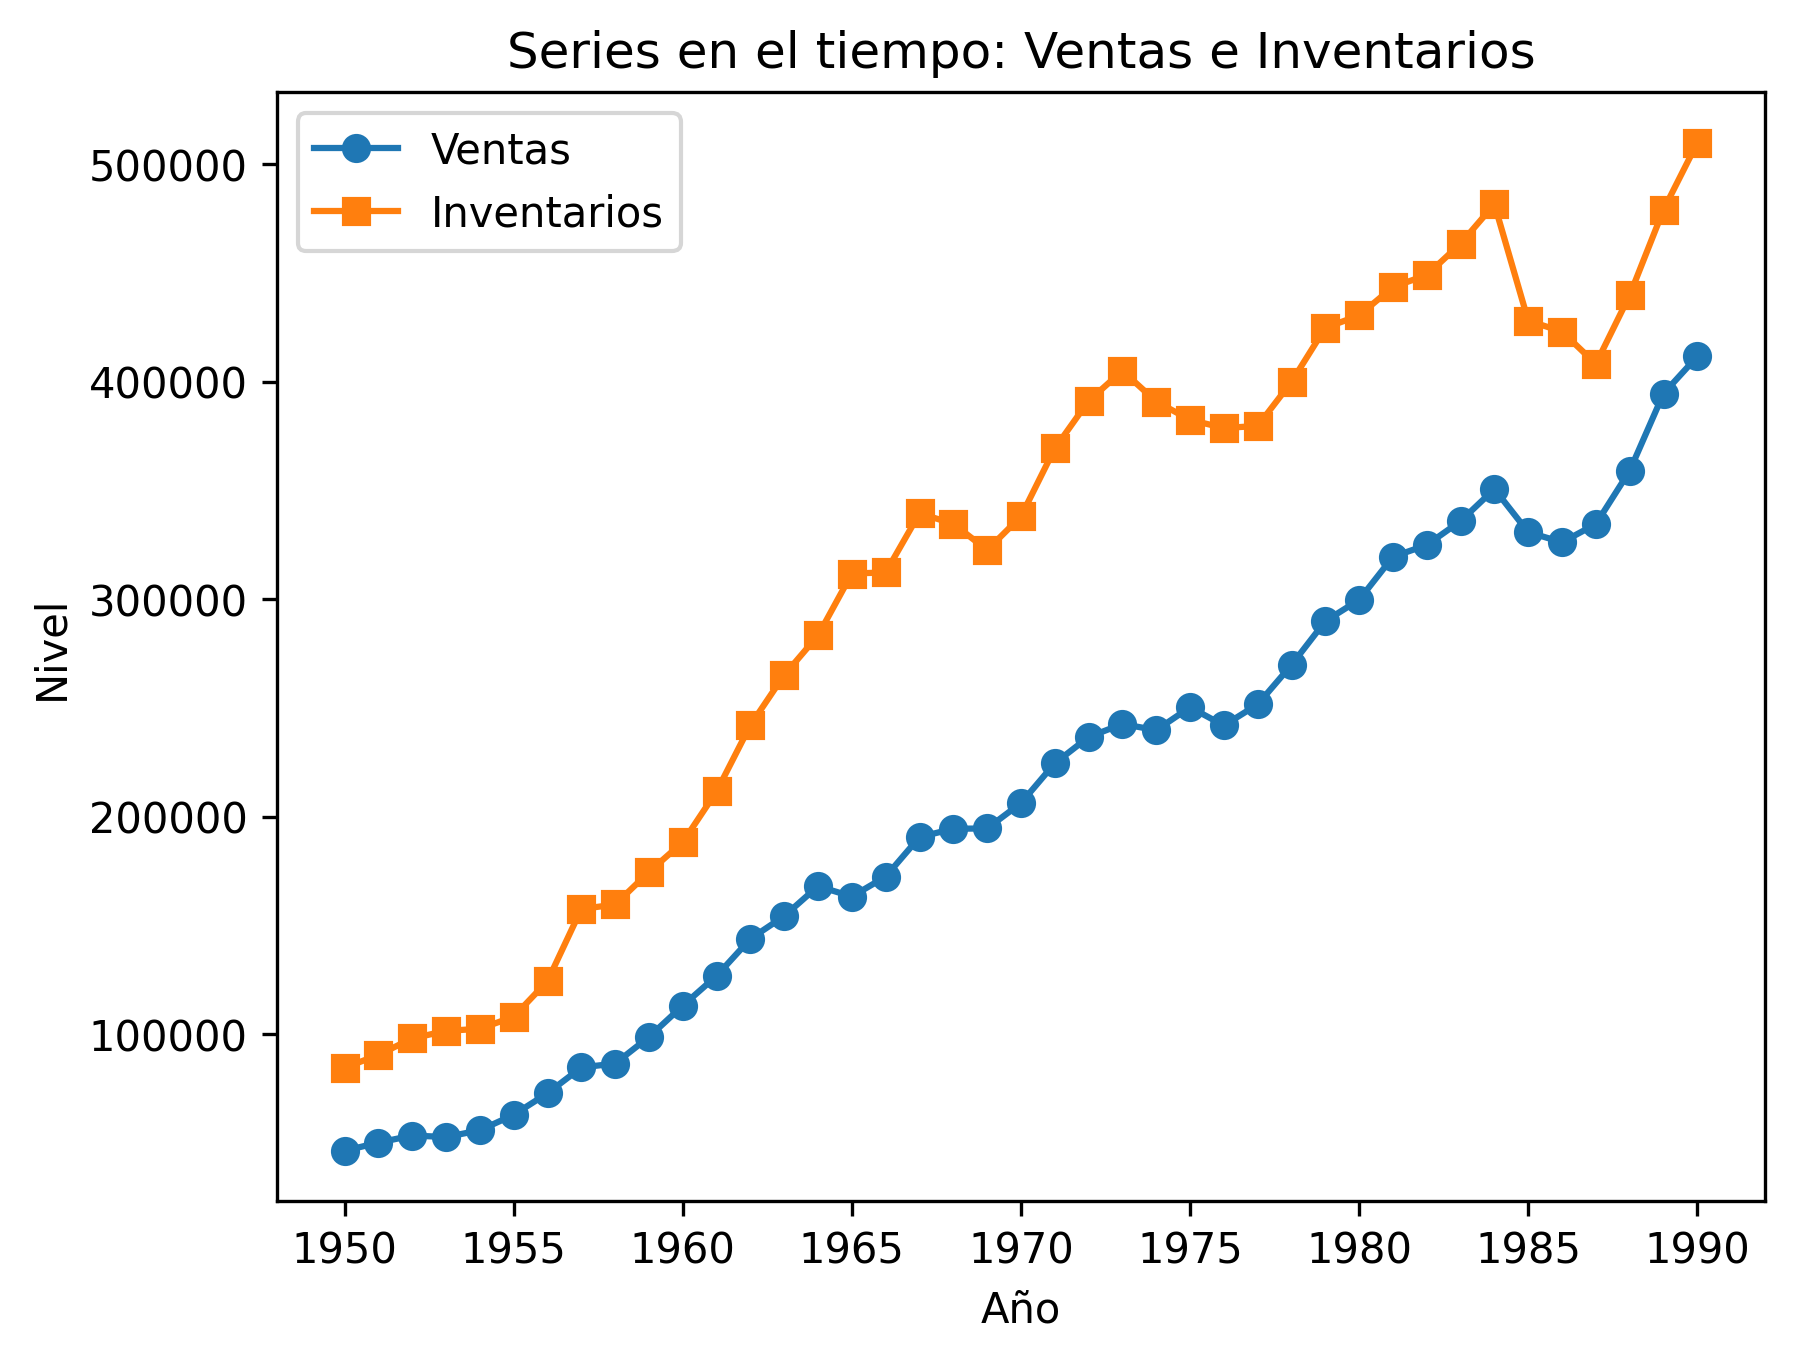
\includegraphics[width=0.75\linewidth]{../plots/python/ex8/ex8_series_ventas_inventarios.png}
    \caption{Series en el tiempo: ventas e inventarios}
\end{figure}
\begin{figure}[H]
    \centering
    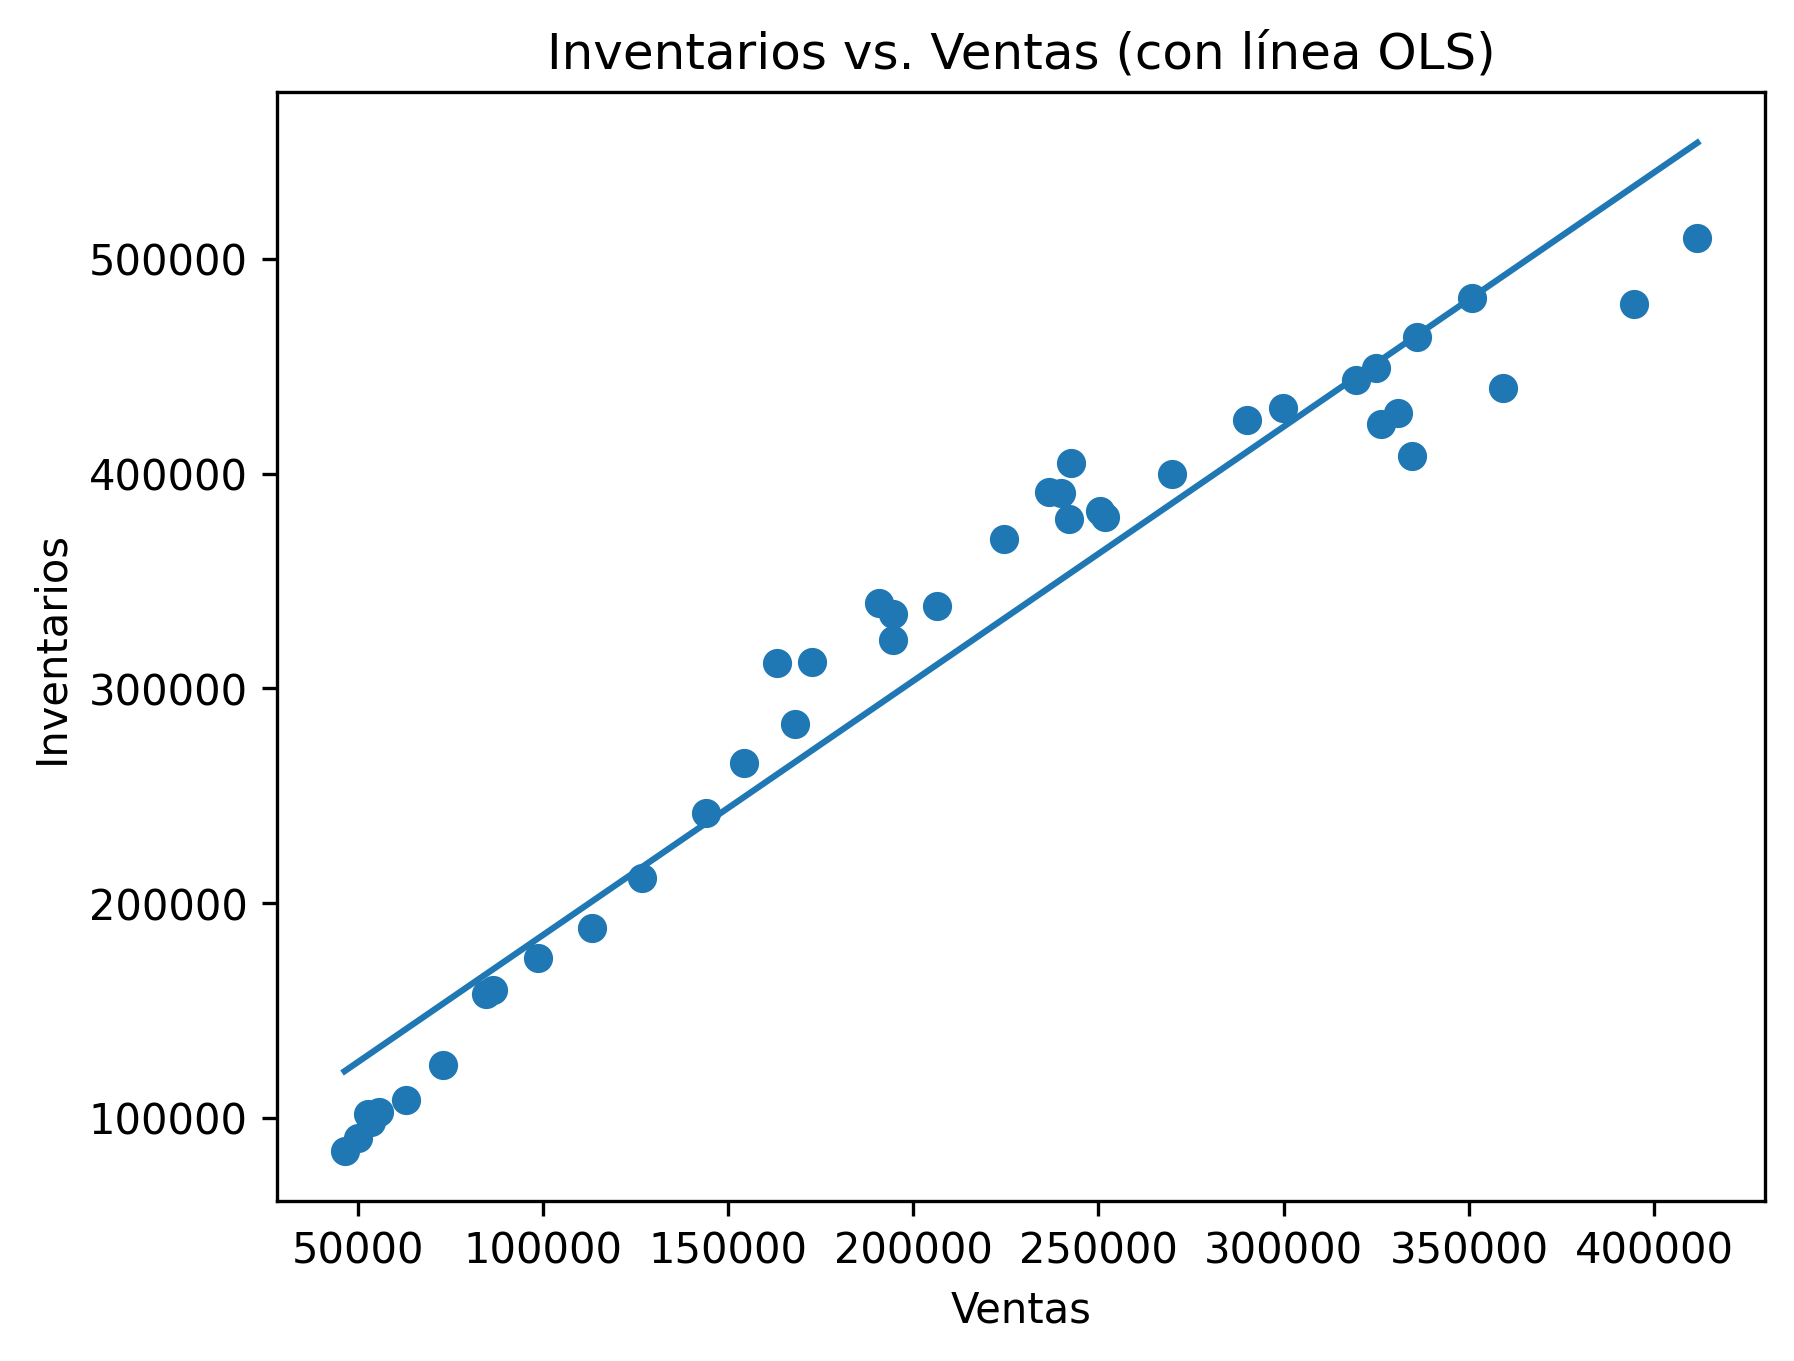
\includegraphics[width=0.6\linewidth]{../plots/python/ex8/ex8_scatter_inv_vs_sales.png}
    \caption{Inventarios vs. ventas con recta OLS}
\end{figure}
\textbf{OLS (Modelo 1).}\\
\begin{table}[H]
\centering
\caption{Resultados OLS: Inventarios sobre Ventas.}
\label{tab:ex8_m1}
\begin{tabular}{lrrrrrr}
\rowcolor{blue!10}
\toprule
\rowcolor{blue!20}
\textcolor{blue}{\textbf{Parámetro}} & \textcolor{blue}{\textbf{Coef}} & \textcolor{blue}{\textbf{EE}} & \textcolor{blue}{\textbf{t}} & \textcolor{blue}{\textbf{p-valor}} & \textcolor{blue}{\textbf{IC 2.5\%}} & \textcolor{blue}{\textbf{IC 97.5\%}} \\
\addlinespace
\rowcolor{blue!10}
\textcolor{blue}{const} & \textcolor{blue}{66669.0} & \textcolor{blue}{10895.7} & \textcolor{blue}{6.12} & \textcolor{blue}{0.000} & \textcolor{blue}{44630.3} & \textcolor{blue}{88707.7} \\
\rowcolor{blue!10}
\textcolor{blue}{sales} & \textcolor{blue}{1.184} & \textcolor{blue}{0.047} & \textcolor{blue}{25.40} & \textcolor{blue}{0.000} & \textcolor{blue}{1.090} & \textcolor{blue}{1.278} \\
\bottomrule
\end{tabular}
\end{table}

\textit{Lectura:} $\hat\beta_2=1.184$ (p$<0.001$), $R^2=0.943$. Sin embargo, veremos abajo que los residuos presentan fuerte dependencia temporal.\\
\textbf{OLS (Modelo 2, con tendencia):}
\begin{equation*}
Y_t = \beta_1 + \beta_2 X_t + \beta_3\,\text{Year}_t + u_t.
\end{equation*}
\begin{table}
\caption{Resultados OLS: Inventarios sobre Ventas y Año.}
\label{tab:ex8_m2}
\begin{tabular}{lrrrrrr}
\toprule
Parámetro & Coef. & E.E. & t & p-valor & IC 2.5% & IC 97.5% \\
\midrule
const & 6057807.2732 & 7324071.9432 & 0.8271 & 0.4133 & -8769001.2248 & 20884615.7711 \\
sales & 1.5234 & 0.4177 & 3.6470 & 0.0008 & 0.6778 & 2.3690 \\
year & -3077.0438 & 3761.6333 & -0.8180 & 0.4185 & -10692.0723 & 4537.9846 \\
\bottomrule
\end{tabular}
\end{table}

El término de tendencia no resulta significativo y no corrige la dependencia temporal.
}

\subsection{Realice las pruebas gráficas de normalidad y de no autocorrelación.}
\textcolor{blue}{
\textbf{Gráficas de residuos (M1 y M2).}
\begin{figure}[H]
    \centering
    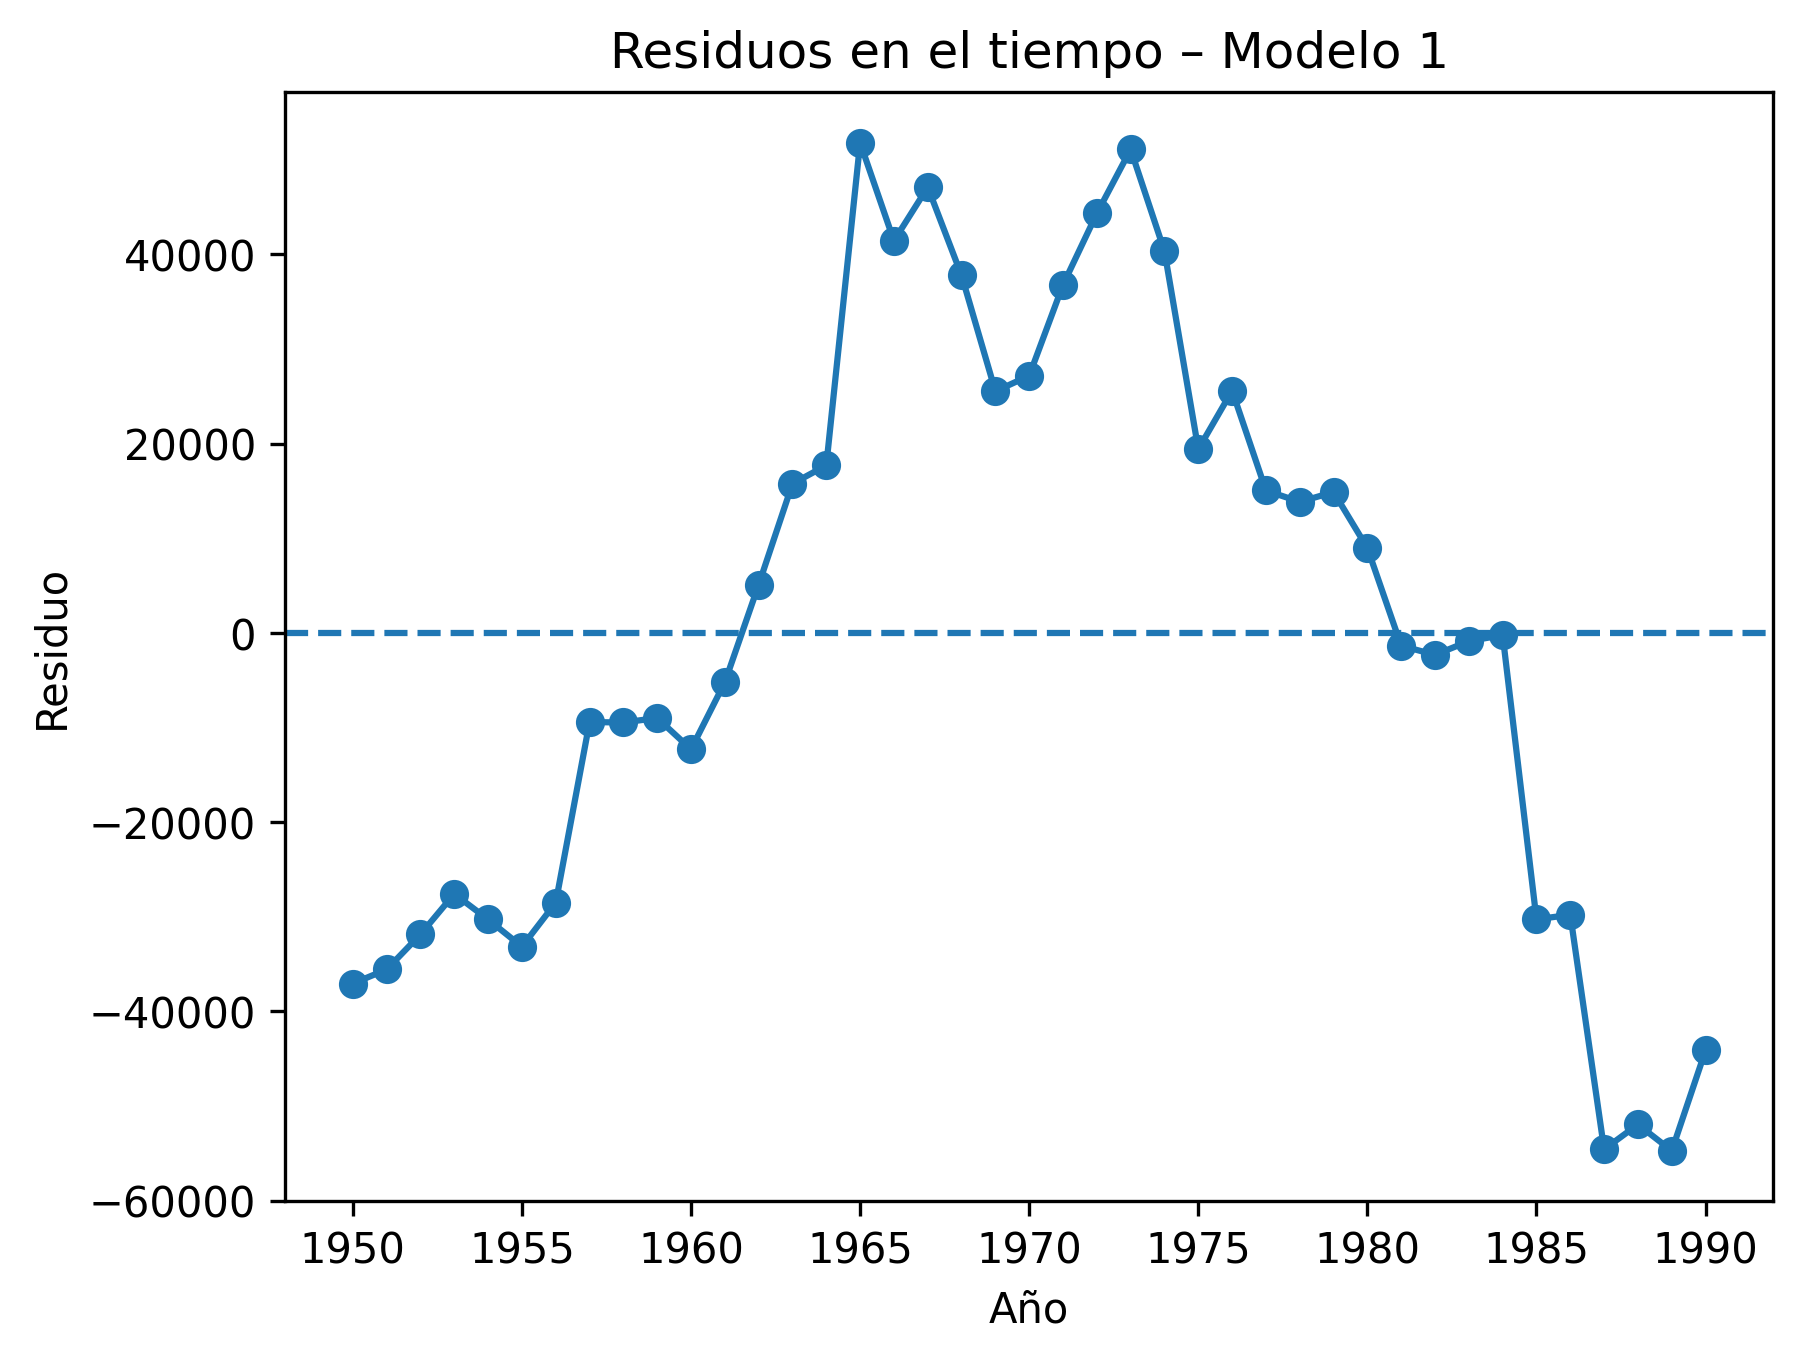
\includegraphics[width=0.7\linewidth]{../plots/python/ex8/ex8_residuos_m1.png}
    \caption{Residuos en el tiempo — Modelo 1}
\end{figure}
\begin{figure}[H]
    \centering
    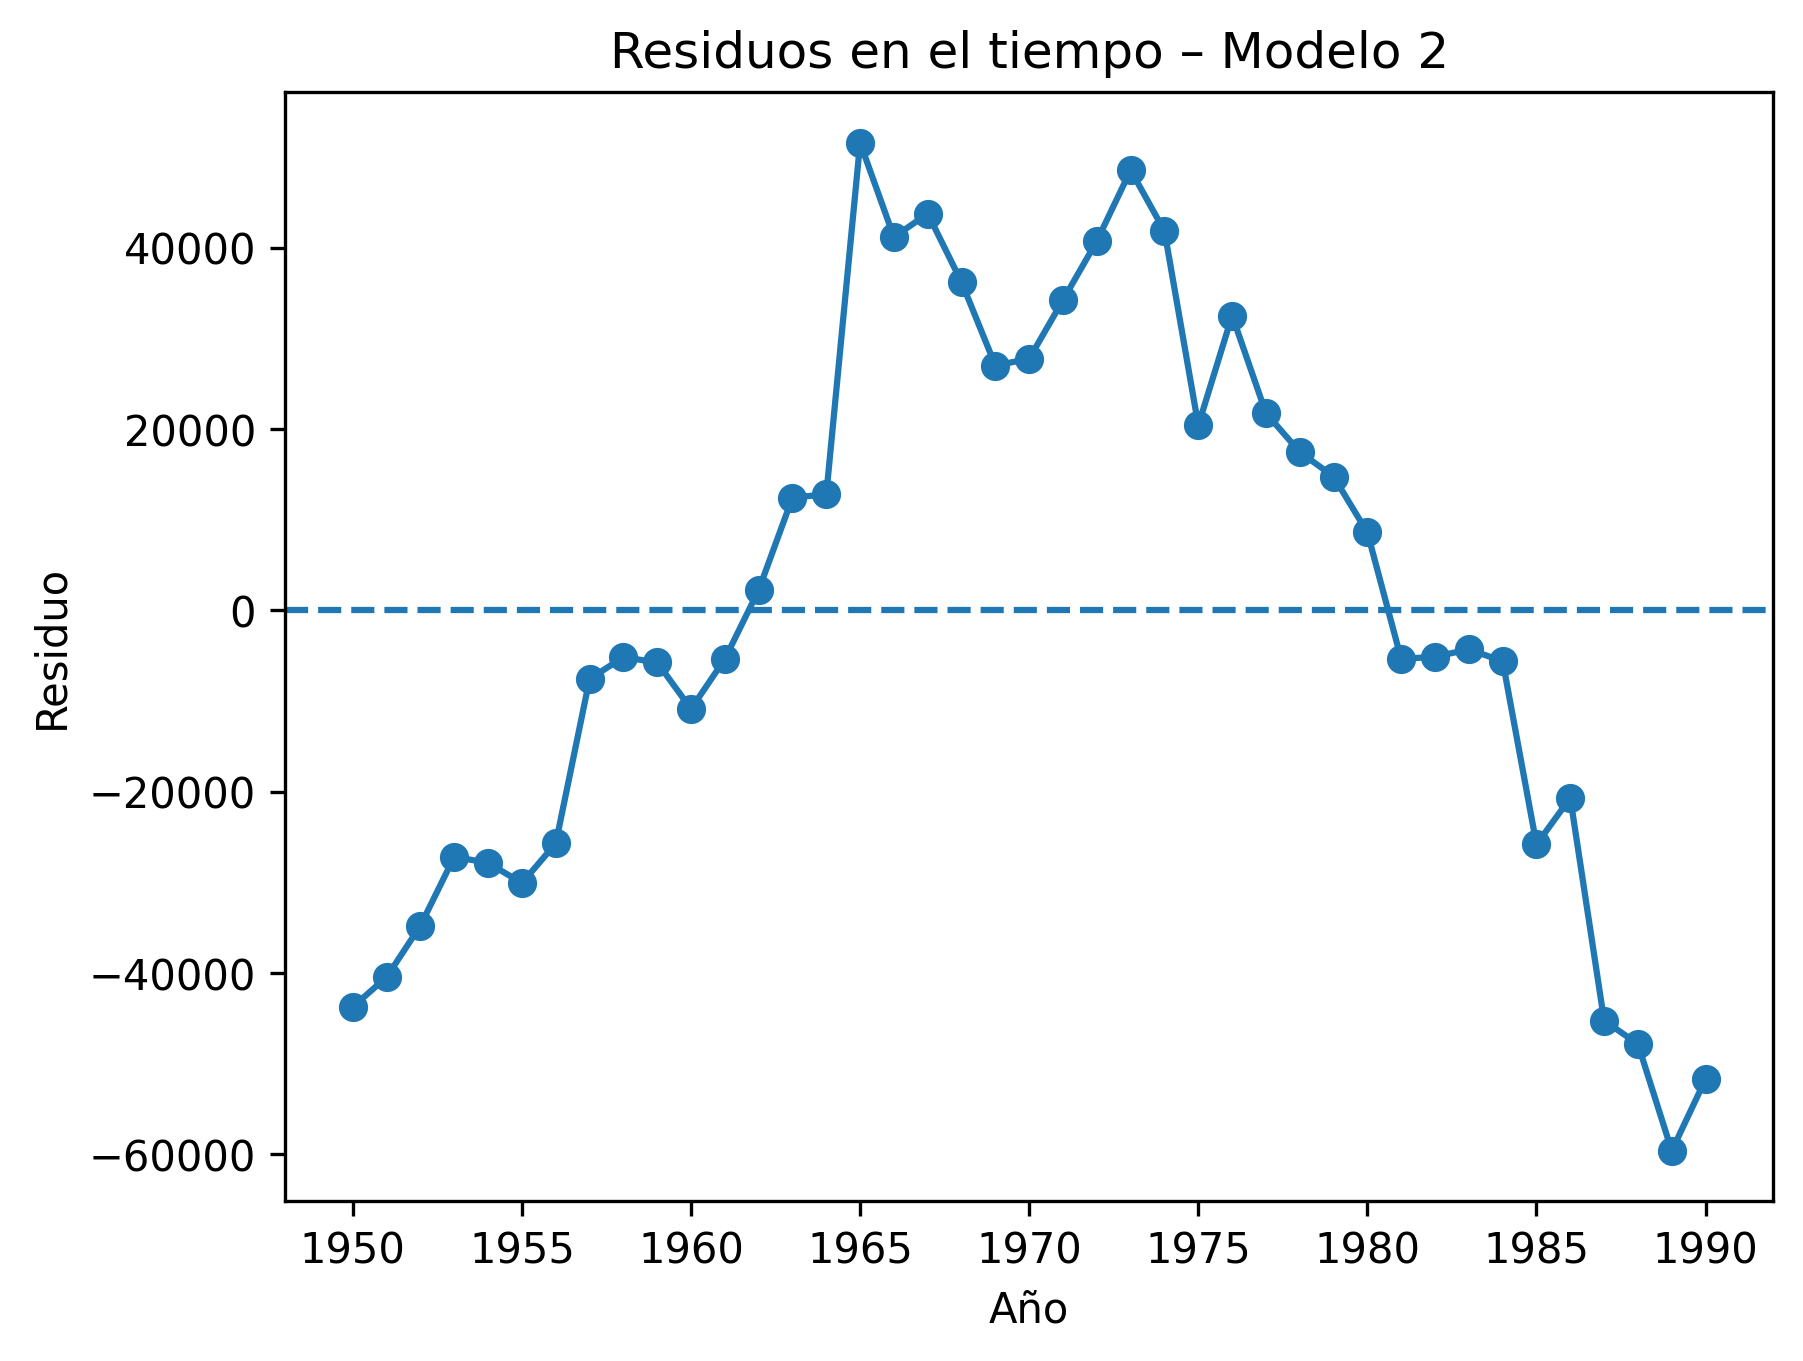
\includegraphics[width=0.7\linewidth]{../plots/python/ex8/ex8_residuos_m2.png}
    \caption{Residuos en el tiempo — Modelo 2}
\end{figure}
\begin{figure}[H]
    \centering
    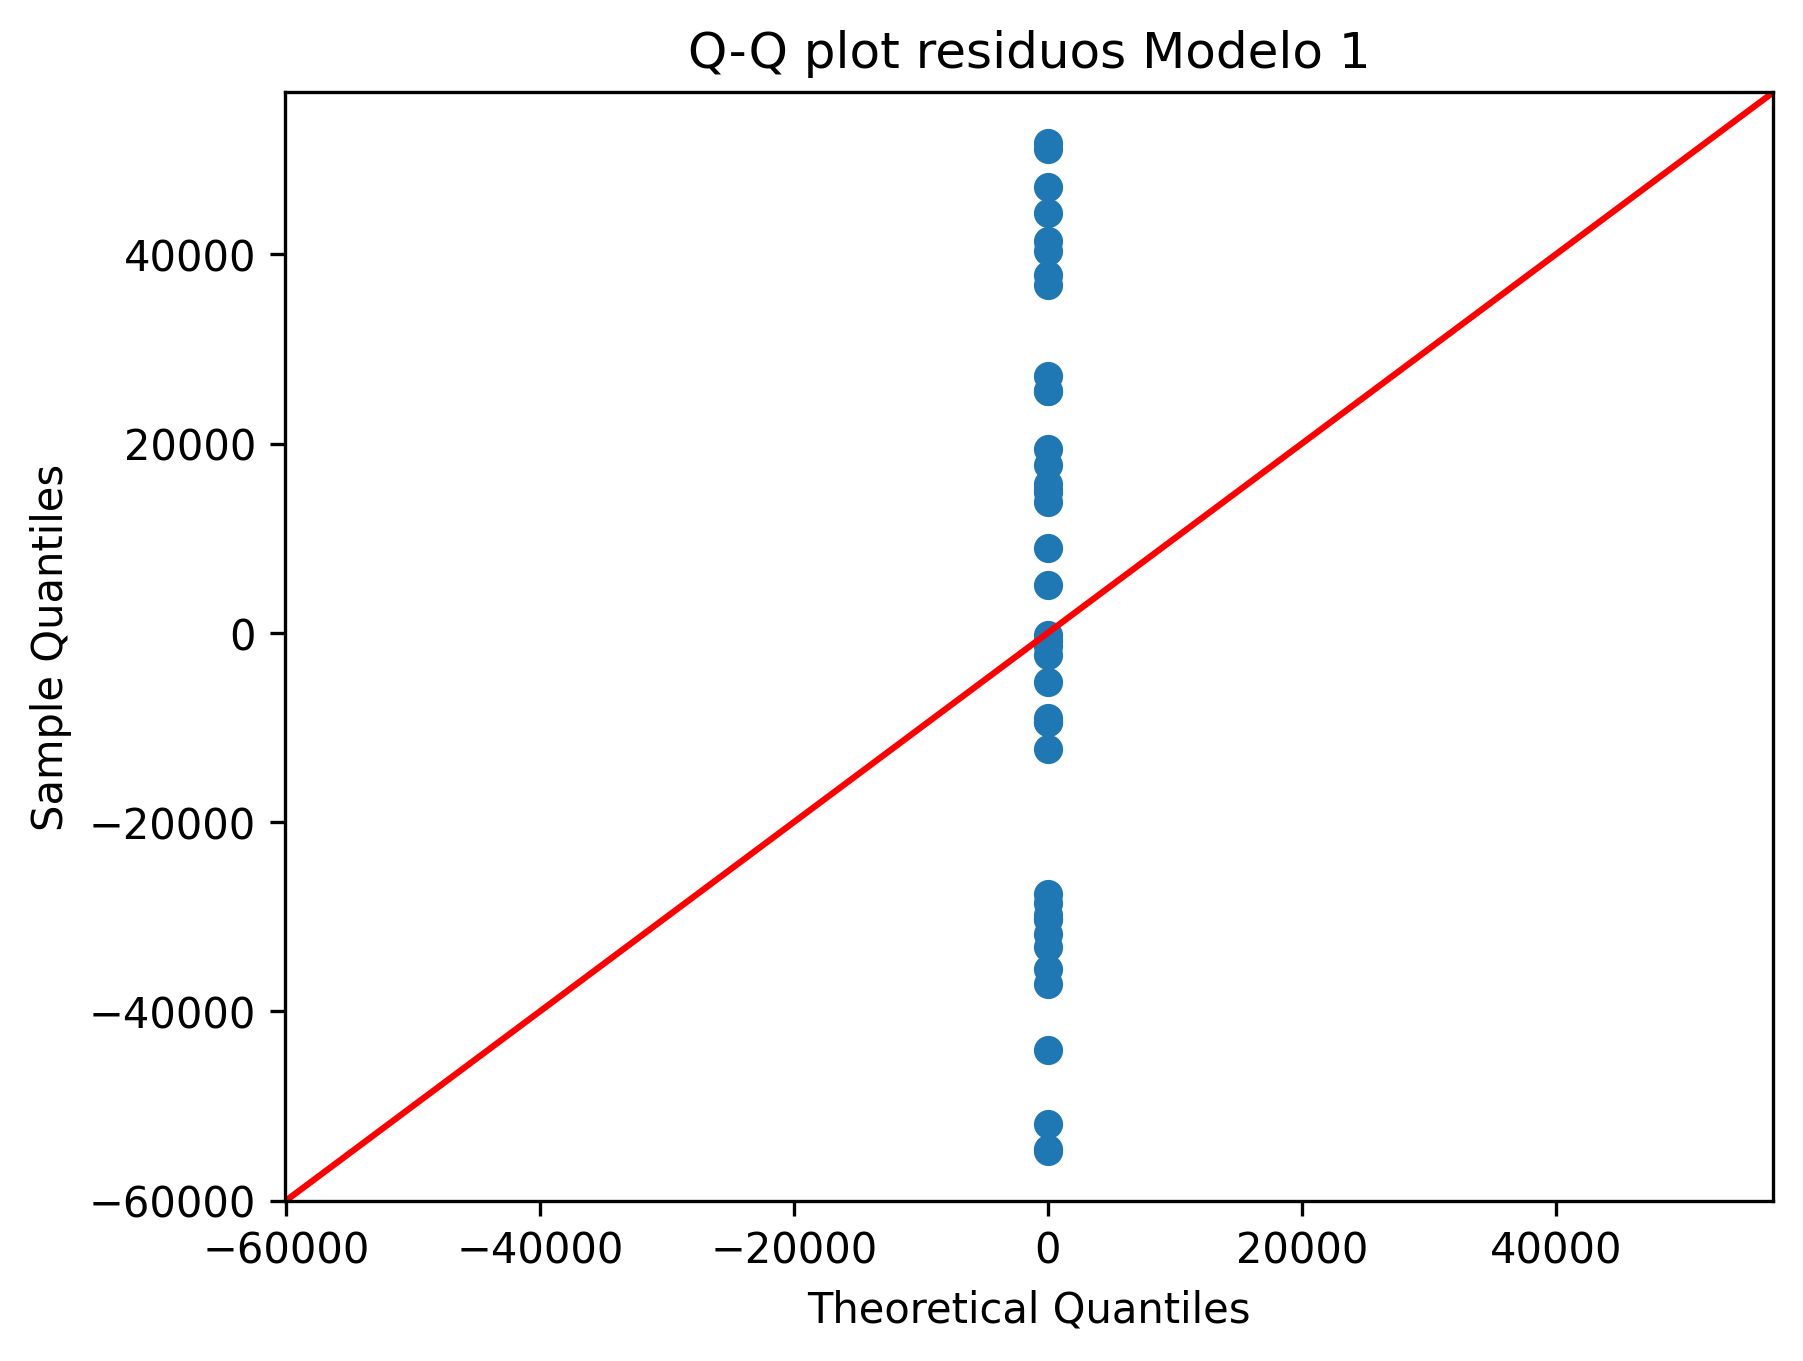
\includegraphics[width=0.48\linewidth]{../plots/python/ex8/ex8_qq_m1.png}\hfill
    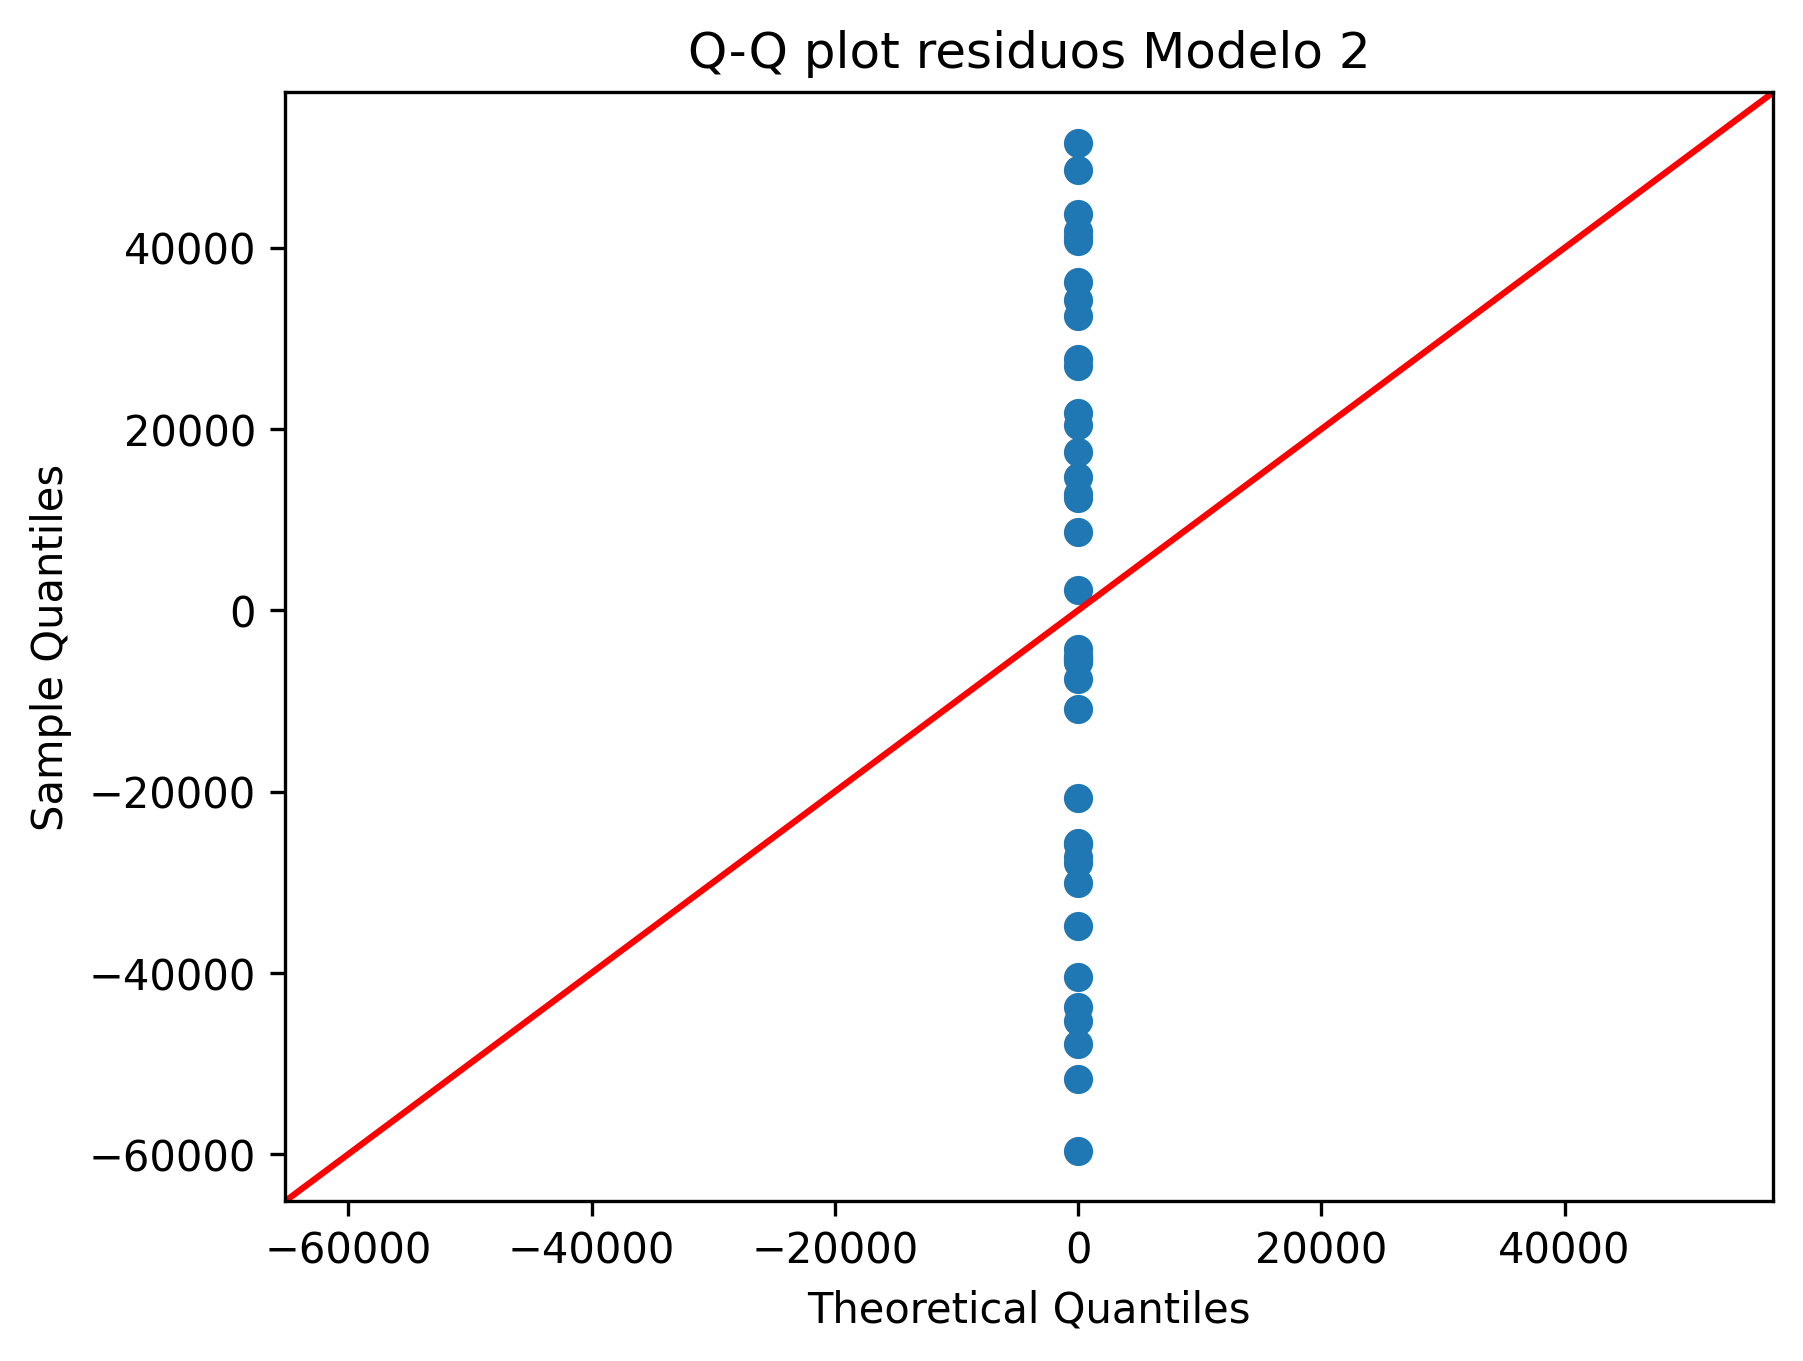
\includegraphics[width=0.48\linewidth]{../plots/python/ex8/ex8_qq_m2.png}
    \caption{QQ-plot de residuos — M1 (izq.) y M2 (der.)}
\end{figure}
\begin{figure}[H]
    \centering
    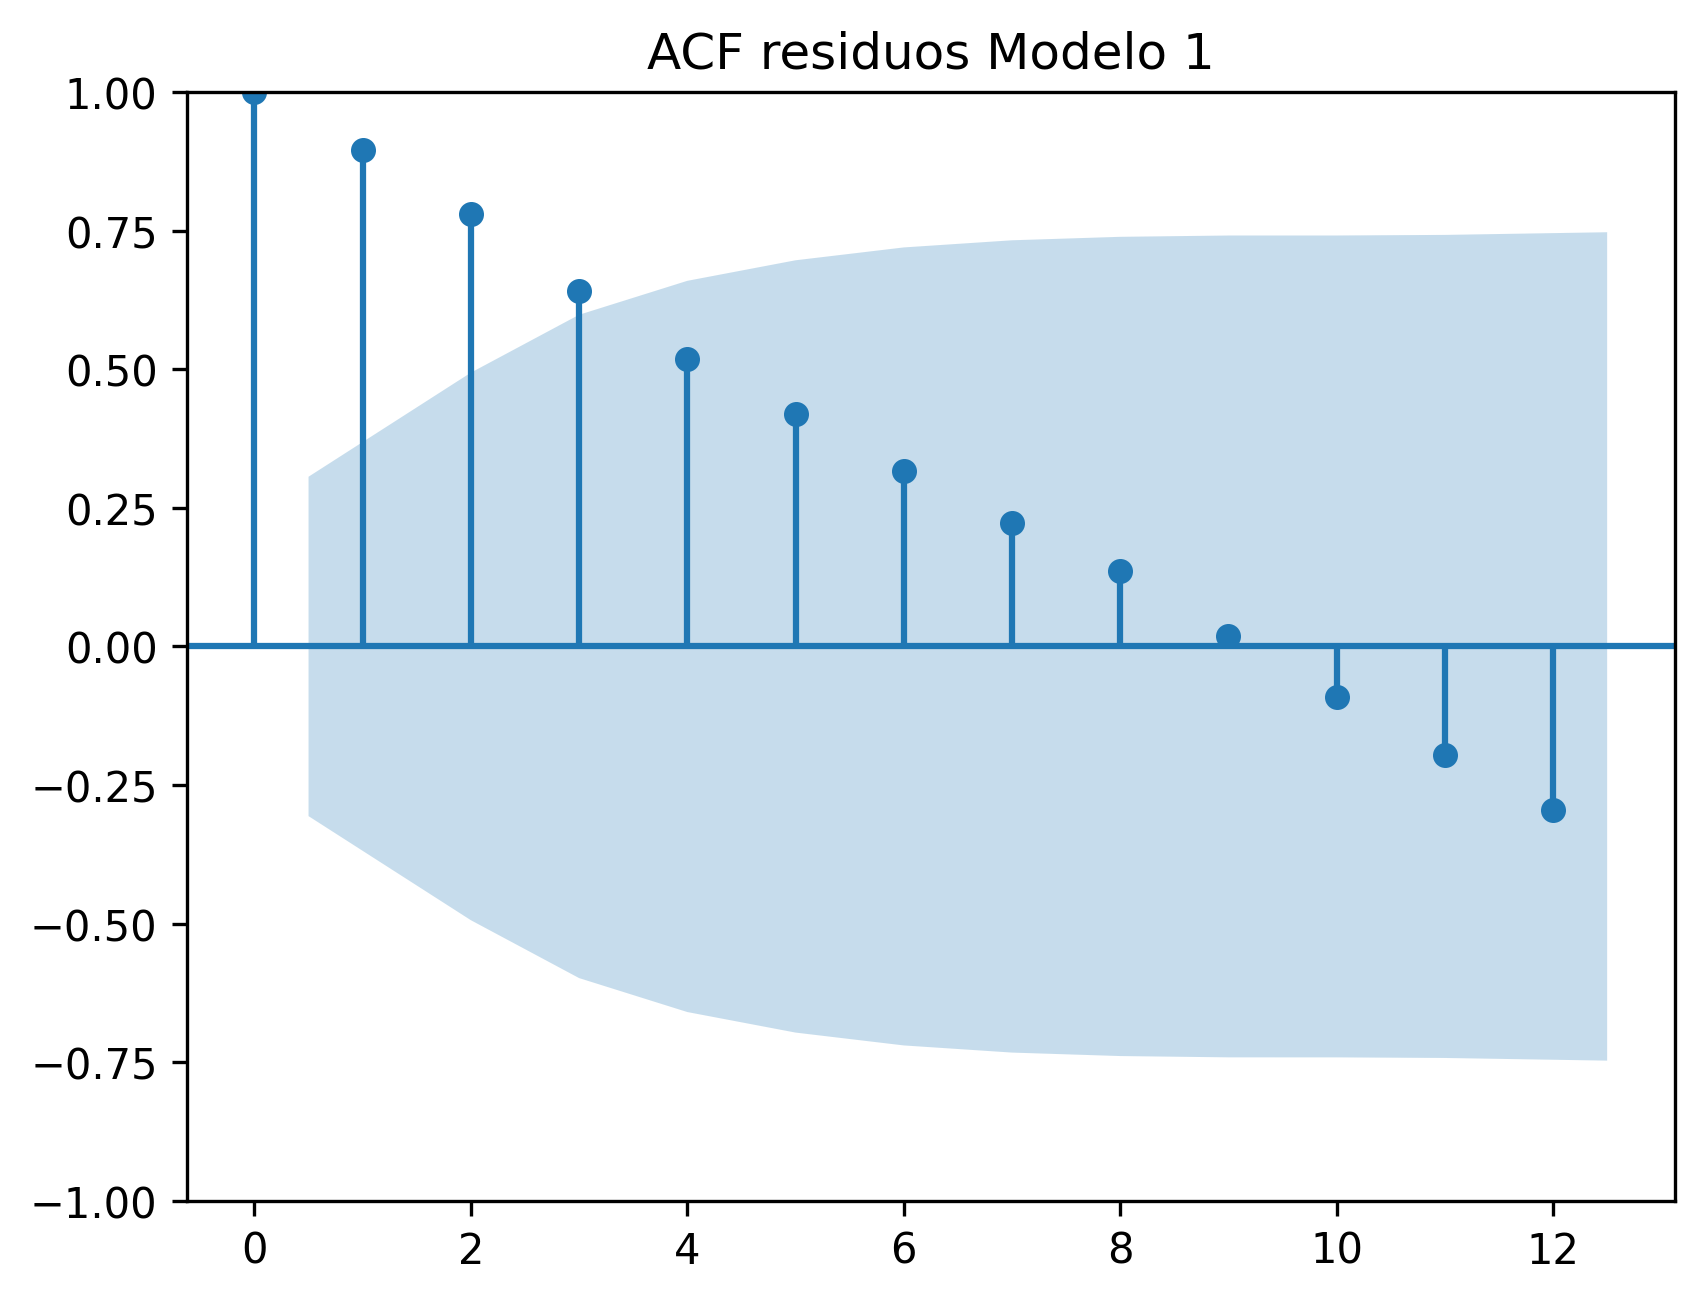
\includegraphics[width=0.48\linewidth]{../plots/python/ex8/ex8_acf_m1.png}\hfill
    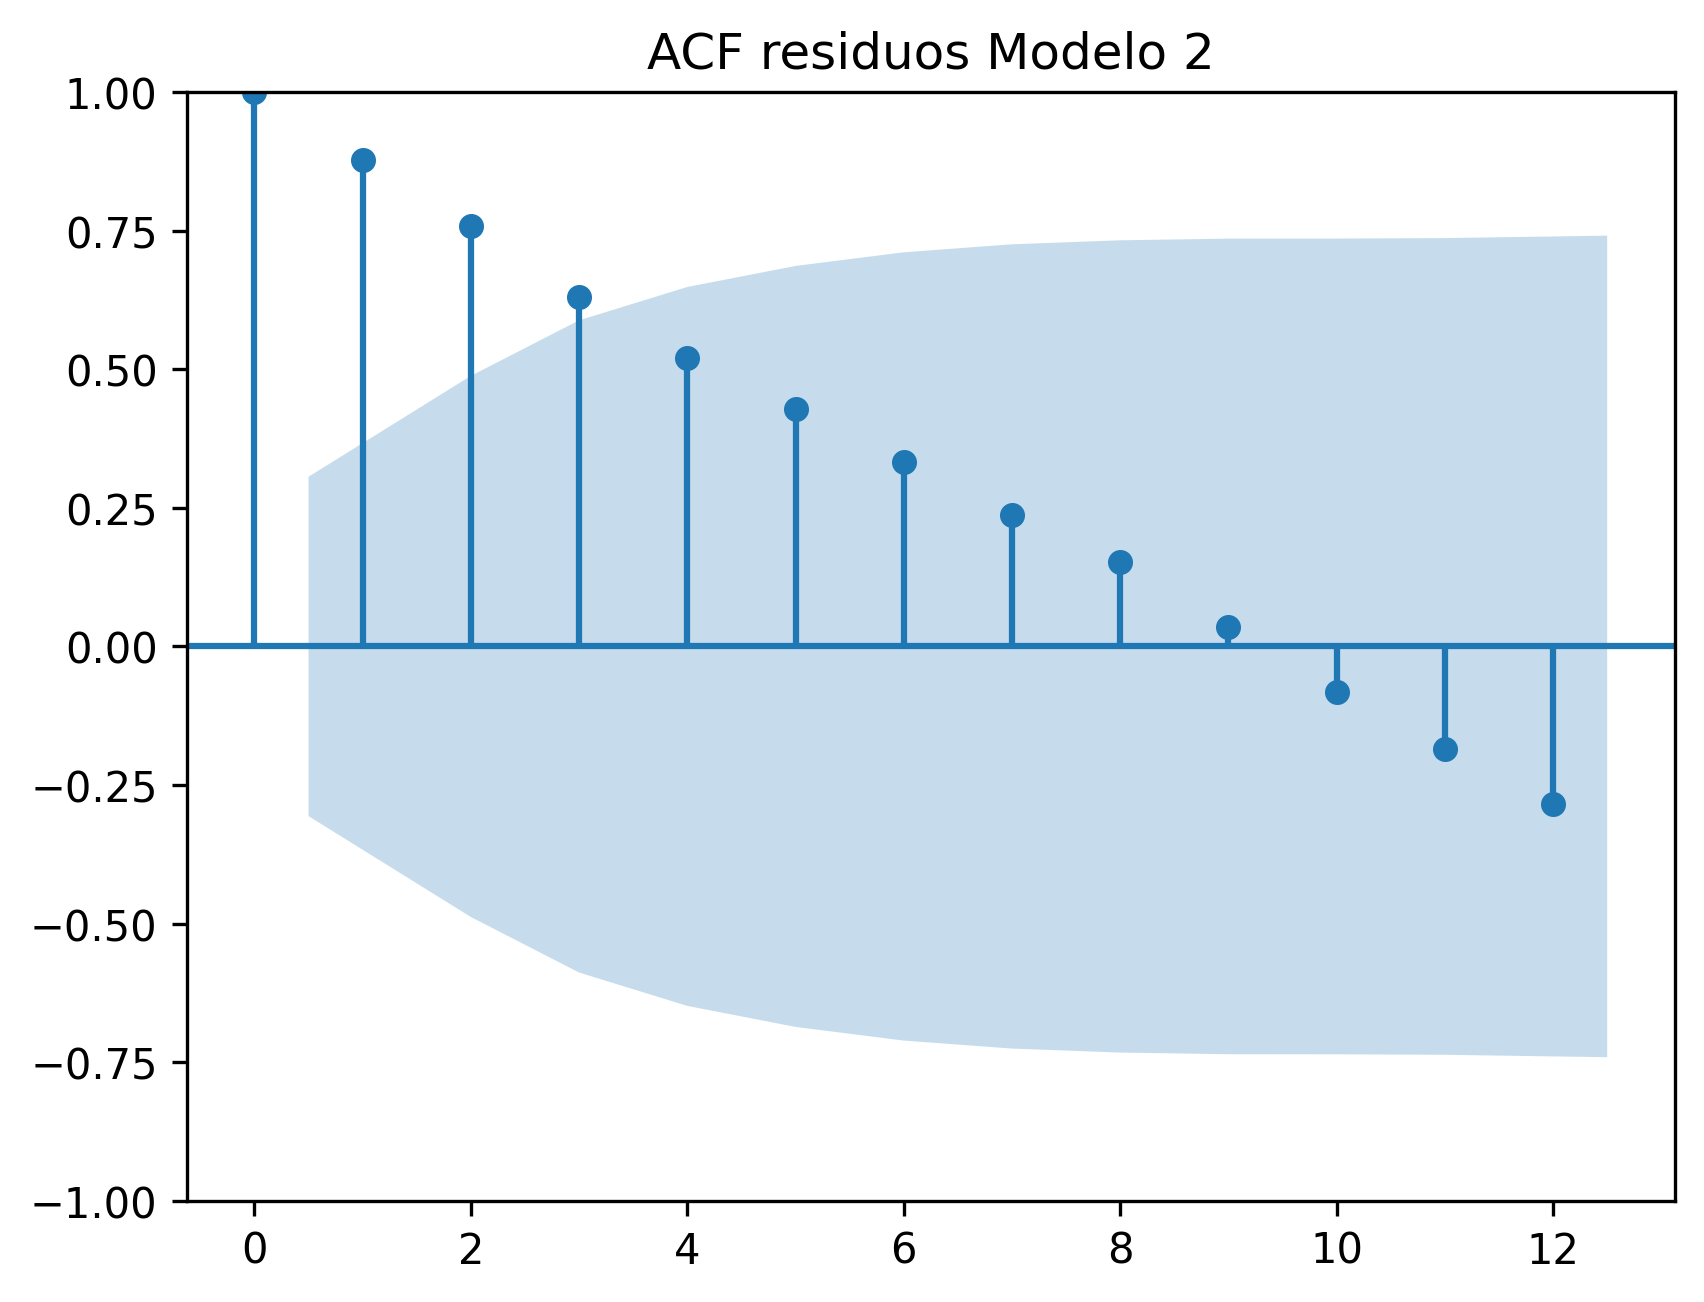
\includegraphics[width=0.48\linewidth]{../plots/python/ex8/ex8_acf_m2.png}
    \caption{ACF de residuos — M1 (izq.) y M2 (der.)}
\end{figure}
Hay rachas largas en el tiempo y barras significativas en la ACF para rezagos bajos $\Rightarrow$ \textbf{autocorrelación positiva}. Los QQ-plots no muestran colas extremas — \textbf{normalidad aceptable}. También es útil observar la evolución de la razón Inventarios/Ventas:
\begin{figure}[H]
    \centering
    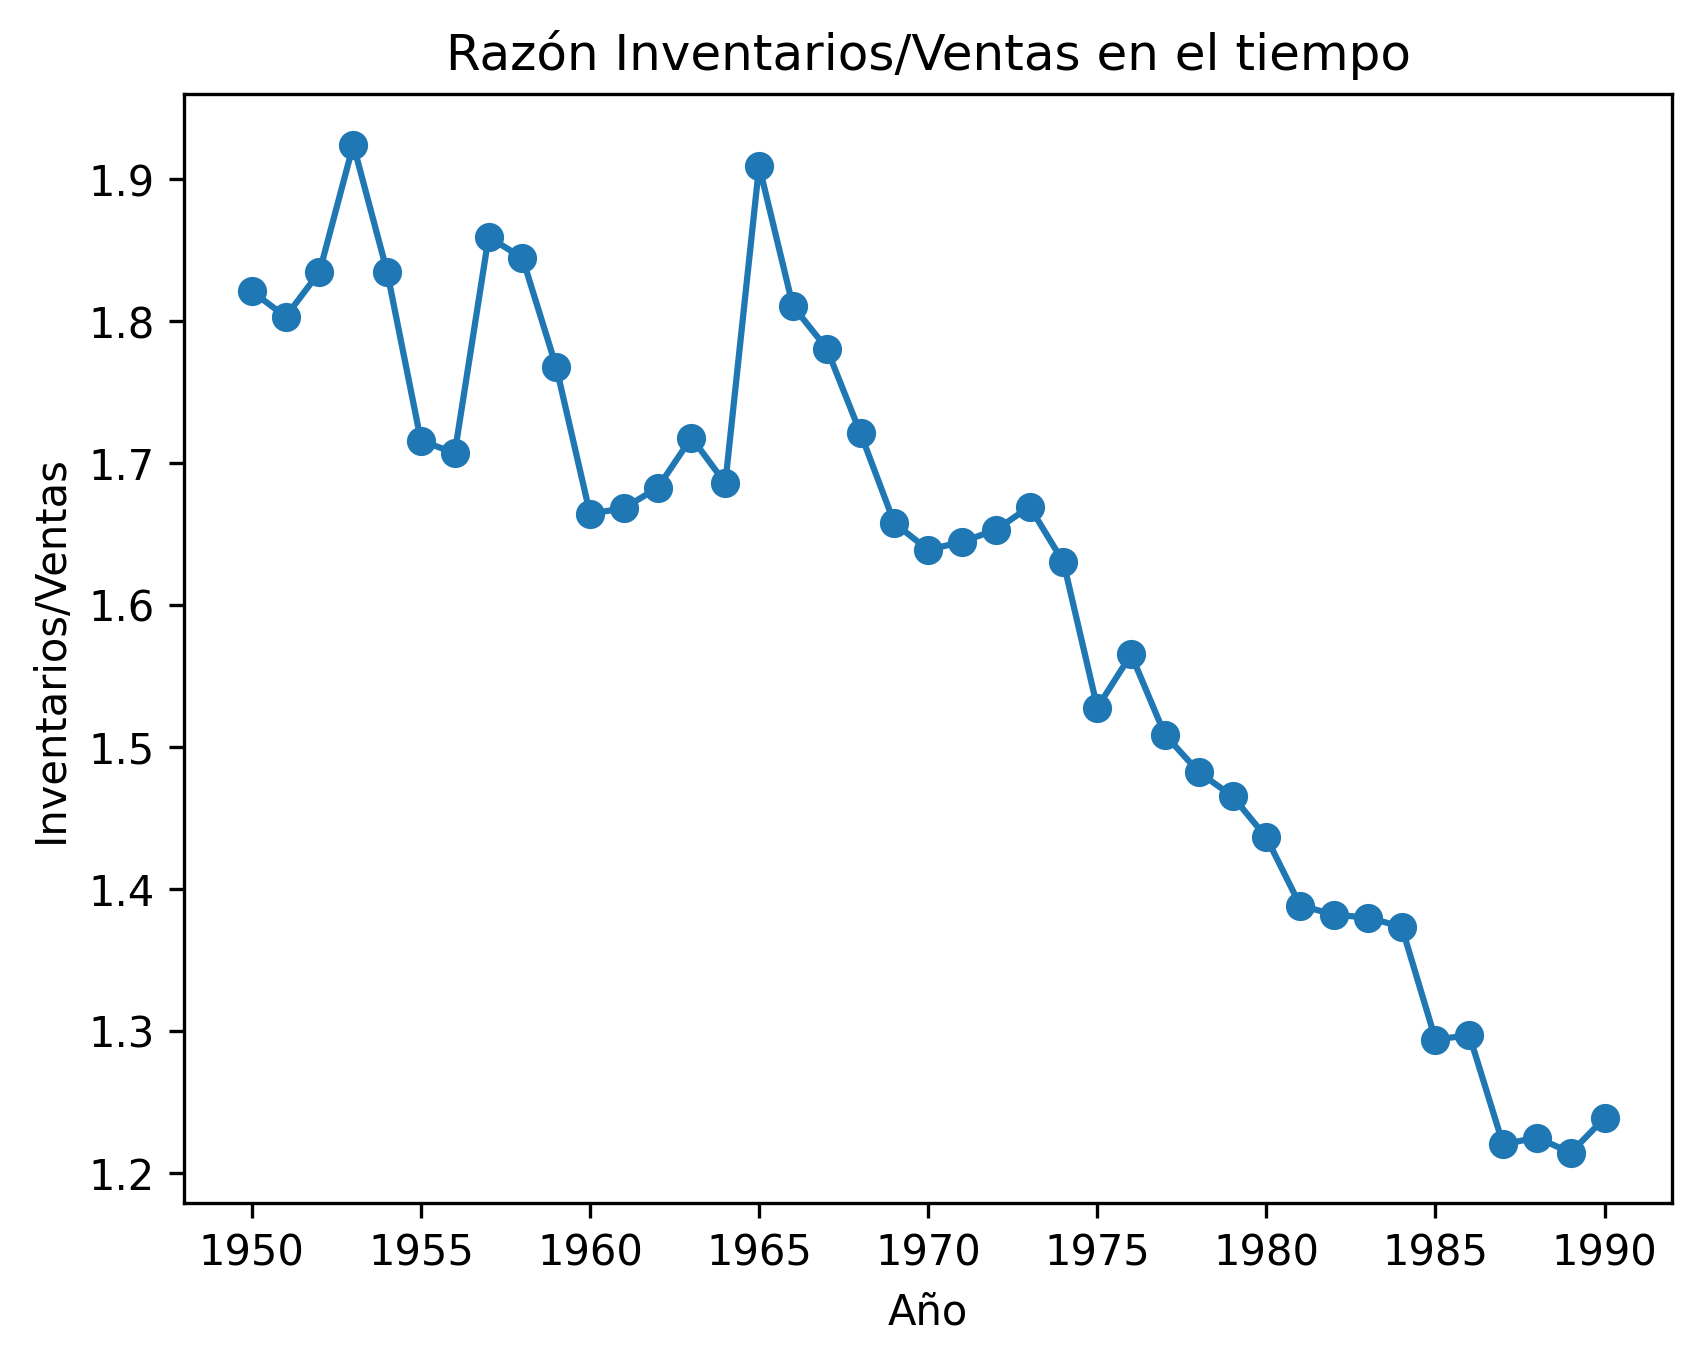
\includegraphics[width=0.6\linewidth]{../plots/python/ex8/ex8_series_ratio.png}
    \caption{Razón Inventarios/Ventas}
\end{figure}
}

\subsection{Con los residuos estimados, investigue si hay autocorrelación positiva mediante i) la prueba de Durbin--Watson y ii) las dos pruebas analíticas de normalidad para los errores poblacionales.}
\textcolor{blue}{
El estadístico de Durbin–Watson (DW) reportado por el script es:
\begin{align*}
DW_{\text{M1}}&=0.1256, & DW_{\text{M2}}&=0.1254.
\end{align*}
Como aproximación, $\hat\rho\approx 1-\tfrac{DW}{2}$ $\Rightarrow$ $\hat\rho\approx 0.94$; valores tan bajos de $DW$ sugieren \textbf{autocorrelación positiva muy fuerte}.\\
Para la normalidad, el script reporta Jarque–Bera (JB): p=0.360 (M1) y p=0.369 (M2), por lo que \textbf{no se rechaza la normalidad} de residuos.\\
Además, el contraste RESET rechaza la especificación (ver cuadro de diagnósticos): hay evidencia de dinámica/curvatura omitida.
\begin{table}
\caption{Pruebas de supuestos y métricas de ajuste para los modelos estimados.}
\label{tab:ex8_diagnosticos}
\begin{tabular}{lrrrrrrrr}
\toprule
Modelo & Durbin–Watson & Breusch–Pagan p & White p & Jarque–Bera p & RESET p & $R^2$ & $R^2$ Ajustado & N \\
\midrule
M1: Inv ~ Ventas & 0.1256 & 0.1819 & 0.2371 & 0.3596 & 0.0000 & 0.9430 & 0.9415 & 41 \\
M2: Inv ~ Ventas + Año & 0.1254 & 0.2126 & 0.1524 & 0.3690 & 0.0000 & 0.9440 & 0.9410 & 41 \\
\bottomrule
\end{tabular}
\end{table}

}
%%%%%%%%%%%%%%%%%%%%%%%%%%%%%%%%%%%%%%%%%%%%%%%%%%%%%%%%%%%%%%%%%%%%%%%%%%%%%%%%%%%%%%%%%%%%%%%%%%%%%%%%%%%%%%
\subsection{Si sospecha que la estructura autorregresiva del error es de orden \texorpdfstring{$p=1$}{p=1}, verifíquelo con la prueba de Breusch--Godfrey.}
    \textcolor{blue}{
        \textbf{Breusch--Godfrey (BG, $p=1$).} El procedimiento consiste en estimar la regresión auxiliar sobre los residuos OLS
        \begin{equation*}
        \hat u_t = \alpha + \gamma_1 X_t + \cdots + \gamma_k Z_{kt} + \phi\,\hat u_{t-1} + v_t,
        \end{equation*}
        (\(Z_{kt}\) son los regresores originales) y contrastar $H_0\!:\ \phi=0$ vía LM $\sim\chi^2_1$.\\[4pt]
        En la tabla \ref{tab:ex8_diagnosticos}, usar las columnas \emph{BG LM p-valor} y \emph{BG F p-valor} para decidir: p-valores pequeños $\Rightarrow$ rechazo de $H_0$ (evidencia de AR(1) positiva), coherente con $DW\approx0.126$ y la ACF.
    }
%%%%%%%%%%%%%%%%%%%%%%%%%%%%%%%%%%%%%%%%%%%%%%%%%%%%%%%%%%%%%%%%%%%%%%%%%%%%%%%%%%%%%%%%%%%%%%%%%%%%%%%%%%%%%%
\subsection{Con base en los resultados de esta prueba, ¿cómo transformaría los datos para eliminar la autocorrelación?}
    \textcolor{blue}{
        Dada la evidencia de AR(1) en los errores, se recomienda estimar por \emph{GLS} tipo Prais--Winsten/Cochrane--Orcutt, aplicando la cuasi-diferenciación
        \begin{equation*}
        Y_t-\rho Y_{t-1} = \beta_1(1-\rho) + \beta_2\,(X_t-\rho X_{t-1}) + \varepsilon_t,
        \end{equation*}
        con $\rho$ estimado (p.ej., por MCO sobre $\hat u_t$ vs. $\hat u_{t-1}$ o por máxima verosimilitud). Como alternativa robusta en presencia de tendencia común, trabajar en diferencias/elasticidades:
        \begin{align*}
        \Delta Y_t &= \beta_2\,\Delta X_t + e_t,\\
        \ln Y_t &= \alpha + \beta\,\ln X_t + u_t. 
        \end{align*}
        En cualquiera de los casos, re-evaluar ACF/PACF y DW, y reportar errores estándar \emph{HAC (Newey--West)} si persiste dependencia débil.
    }
%%%%%%%%%%%%%%%%%%%%%%%%%%%%%%%%%%%%%%%%%%%%%%%%%%%%%%%%%%%%%%%%%%%%%%%%%%%%%%%%%%%%%%%%%%%%%%%%%%%%%%%%%%%%%%
%%%%%%%%%%%%%%%%%%%%%%%%%%%%%%%%%%%%%%%%%%%%%%%%%%%%%%%%%%%%%%%%%%%%%%%%%%%%%%%%%%%%%%%%%%%%%%%%%%%%%%%%%%%%%%
\section{Link al repositorio con código fuente}
\url{https://github.com/enriquegomeztagle/MCD-Econometria/tree/main/HWs/RegressionAssumptions}
%%%%%%%%%%%%%%%%%%%%%%%%%%%%%%%%%%%%%%%%%%%%%%%%%%%%%%%%%%%%%%%%%%%%%%%%%%%%%%%%%%%%%%%%%%%%%%%%%%%%%%%%%%%%%%
%%%%%%%%%%%%%%%%%%%%%%%%%%%%%%%%%%%%%%%%%%%%%%%%%%%%%%%%%%%%%%%%%%%%%%%%%%%%%%%%%%%%%%%%%%%%%%%%%%%%%%%%%%%%%%
\end{document}
